\documentclass[12pt, a4paper, titlepage]{report}
\usepackage[a4paper,top=2.5cm,bottom=2cm,left=2cm,right=2cm]{geometry}
\usepackage[italian]{babel}
\usepackage[hidelinks]{hyperref}
\usepackage{graphicx}
\usepackage{algorithm}
\usepackage{capt-of}
\usepackage{amsmath}
\usepackage{longtable}
\usepackage{caption}
\usepackage{booktabs}
\usepackage{algpseudocode}
\usepackage{makecell}
\usepackage[utf8]{inputenc}
\usepackage{fixltx2e}
\usepackage{listings}
\usepackage{hyperref}
\usepackage{makecell}
\usepackage{changepage}
\usepackage{paracol}
\usepackage{siunitx}
\usepackage{lipsum}

\usepackage[swapnames]{frontespizio}

\usepackage{fancyhdr}
\usepackage{lastpage}
%\pagestyle{fancy}
%\fancyhf{}
%\cfoot{Pagina \thepage\ di \pageref{LastPage}}
%\author{Alberto Bezzon, Tommaso Carraro} \title{Contingency Plan} \date{\today}

\setcounter{tocdepth}{6}
\setcounter{secnumdepth}{6}
\newcommand\tab[1][1cm]{\hspace*{#1}}
\renewcommand{\thesection}{\arabic{section}}%
\newcommand{\myparagraph}[1]{\paragraph{#1}\mbox{} \mbox{}}
\newcommand{\vendor}{Acronis} %è la ditta fornitrice di hw
\newcommand{\backupVendor}{ExaGrid} %è la ditta fornitrice di backup
\newcommand{\vaultVendor}{EVault} %è la ditta fornitrice del servizio vaulting
\newcommand{\hotVendor}{Recovery Point} % ditta che fornisce l'hot site
\newcommand{\tommaso}{Tommaso Carraro}
\newcommand{\alberto}{Alberto Bezzon}

%comandi per le procedure dei team di ripristino
\newcommand{\procTeam}[1]{\item \textbf{Procurement Team}:
			\begin{itemize}
				\item Il team deve contattare la ditta \vendor;
				\item Il team deve ordinare l'hardware necessario per il funzionamento del sistema #1;
				\item Il team deve accordarsi con \vendor{} per avere le risorse richieste in tempi brevi.
			\end{itemize}
}
\newcommand{\softTeam}[1]{\item \textbf{Software Team}:
			\begin{itemize}
				\item Il team deve organizzare i supporti di backup ricevuti dall'azienda \backupVendor;
				\item Il team deve inserire nell'inventario e controllare l'accesso ai supporti di archiviazione;
				\item Il team deve ripristinare i file di dati del software del sistema #1;
				\item Il team deve ripristinare i file di dati del software delle applicazioni utili al funzionamento del sistema #1.
			\end{itemize}}
\newcommand{\hardTeam}[1]{\item \textbf{Hardware Team}:
			\begin{itemize}
				\item Il team deve verificare i requisiti di occupazione in sospeso con il sito;
				\item Il team deve ispezionare lo spazio fisico per l'installazione dei sistemi necessari a supportare il sistema #1;
				\item Il team deve coordinare il trasporto dell'attrezzatura dalla ditta \vendor;
				\item  Il team deve garantire l'installazione dei terminali temporanei e delle workstation necessari collegati all'hardware del sito;
				\item Il team deve pianificare e coordinare l'installazione dei sistemi necessari nel sito.
			\end{itemize}}
\newcommand{\offTeam}[1]{\item \textbf{Off-site Storage Team}:
			\begin{itemize}
				\item Il team deve mettersi in contatto con l'azienda venditrice di backup \backupVendor;
				\item Il team deve richiedere i backup del sistema #1;
				\item Il team deve richiedere i backup delle applicazioni utili alla gestione del sistema #1;
				\item Il team deve coordinare il trasporto dei supporti di backup richiesti verso il sito;
				\item Una volta che i supporti sono arrivati, il team deve predisporli all'utilizzo.
			\end{itemize}}
\newcommand{\serverTeam}[1]{\item \textbf{Server Recovery Team}:
			\begin{itemize}
				\item Il team deve verificare se esistono configurazioni standard per il server che ospita l'applicazione #1;
				\item Il team deve configurare il server che ospita l'applicazione #1 una volta che esso viene installato dall'Hardware Team.
			\end{itemize}}
\newcommand{\systTeam}[1]{\item \textbf{Systems Software Team}:
			\begin{itemize}
				\item Il team deve caricare e provare il sistema operativo sui sistemi installati;
				\item Il team deve recuperare le immagini di sistema dai supporti di backup e installarle sui sistemi che ospiteranno l'applicazione #1;
				\item Il team deve installare il sistema #1 recuperato dall'Off-site Storage Team sui sistemi installati e deve ripristinarne i dati.
			\end{itemize}}
\newcommand{\testTeam}[1]{\item \textbf{Test Team}:
			\begin{itemize}
				\item Il team deve verificare il corretto funzionamento dell'hardware installato per il sistema #1;
				\item Il team deve verificare il corretto funzionamento del software del sistema #1;
				\item Il team deve verificare il corretto funzionamento delle applicazioni utili alla gestione del sistema #1;
				\item Il team deve verificare che il ripristino proceda correttamente;
				\item Il team deve verificare periodicamente che il sito funzioni correttamente.
			\end{itemize}}
\newcommand{\lanTeam}[1]{\item \textbf{LAN Recovery Team}:
			\begin{itemize}
				\item Il team deve verificare che l'infrastruttura di rete del sito sia sufficiente a poter collegare il server #1 alla rete del sito principale;
				\item Nel caso in cui manchino apparecchiature di rete, il team si deve occupare di contattare il Procurement Team per il recupero dell'attrezzatura necessaria;
				\item Nel caso in cui l'attrezzatura presente sul sito sia sufficiente, il team deve collegare il sistema #1 alla infrastruttura di rete e reinstradare le comunicazioni dati verso il sito principale;
				\item Il team deve ristabilire i controlli degli accessi alla rete sul server;
				\item Il team deve contattare il Test Team perché gli opportuni controlli di connessione vengano eseguiti.
			\end{itemize}}
			
			%%%%%%%%%%%%%%%%%%%%%%%%%%%%%%%%%%%%%%%%%%%%%%%%%%%%%%%%%%%%%%%%%%%%%%%%%%%%%% Procedure per il ritorno alla normalità
			
\newcommand{\procRANTeam}[1]{\item \textbf{Procurement Team}:
			\begin{itemize}
				\item Il team deve contattare la ditta \vendor;
				\item Il team deve ordinare l'hardware necessario per la ricostruzione del sistema #1;
				\item Il team deve accordarsi con \vendor{} per avere le risorse richieste in tempi brevi.
			\end{itemize}
}
			
\newcommand{\hardRANTeam}[1]{\item \textbf{Hardware Team}:
	\begin{itemize}
				\item Il team deve ispezionare lo spazio fisico per la ricostruzione dei sistemi che supportano il sistema #1;
				\item Il team deve coordinare il trasporto dell'attrezzatura dalla ditta \vendor;
				\item Il team deve pianificare e coordinare l'installazione dei sistemi da ricostruire.
	\end{itemize}
}

\newcommand{\serverRANTeam}[1]{\item \textbf{Server Recovery Team}:
	\begin{itemize}
		\item Il team deve verificare se esistono configurazioni standard per il server che ospita l'applicazione #1;
		\item Il team deve configurare il server che ospita l'applicazione #1 una volta che esso viene ricostruito dall'Hardware Team.
	\end{itemize}
}

\newcommand{\lanRANTeam}[1]{\item \textbf{LAN Recovery Team}:
	\begin{itemize}
				\item Il team deve verificare se l'infrastruttura di rete del sito é ancora funzionante per poter collegare il server #1 alla rete;
				\item Nel caso in cui delle apparecchiature di rete debbano essere ricostruite, il team si deve occupare di contattare il Procurement Team per il recupero dell'attrezzatura necessaria;
				\item Una volta che l'attrezzatura di rete si trova in uno stato funzionante, il team deve collegare il sistema #1 all'infrastruttura di rete e reinstradare le comunicazioni dati;
				\item Il team deve ristabilire i controlli degli accessi alla rete sul server.
			\end{itemize}
}
			
\newcommand{\testRANTeam}[1]{\item \textbf{Test Team}:
			\begin{itemize}
				\item Il team deve verificare il corretto funzionamento dell'hardware ricostruito per il sistema #1;
				\item Il team deve verificare che la ricostruzione proceda correttamente;
				\item Il team deve verificare che il server #1 sia correttamente collegato alla rete del sito.
			\end{itemize}
}
			
\newcommand{\ricostruzione}[1]{
Le seguenti procedure delineano i passi necessari per la ricostruzione del sistema #1 presso il sito principale, in modo da permettere alle normali operazioni eseguite dal sistema #1 di essere trasferite dal sito alternativo a quello principale:
	\begin{enumerate}
		\procRANTeam{#1}
		\hardRANTeam{#1}
		\serverRANTeam{#1}
		\lanRANTeam{#1}
		\testRANTeam{#1}
	\end{enumerate}		
}
			
			%%%%%%%%%%%%%%%%%%%%%%%%%%%%%%%%%%% procedure trasferimento
			
\newcommand{\offRANTeam}[1]{\item \textbf{Off-site Storage Team}:
	\begin{itemize}
		\item Il team deve mettersi in contatto con il sito alternativo per il trasferimento dei supporti di backup più recenti;
		\item Il team deve richiedere i backup del sistema #1;
		\item Il team deve richiedere i backup delle applicazioni utili alla gestione del sistema #1;
		\item Il team deve coordinare il trasporto dei supporti di backup richiesti verso il sito principale o il nuovo sito;
		\item Una volta che i supporti sono arrivati, il team deve predisporli all'utilizzo.
	\end{itemize}
}

\newcommand{\softRANTeam}[1]{\item \textbf{Software Team}:
			\begin{itemize}
				\item Il team deve organizzare i supporti di backup ricevuti dal sito alternativo;
				\item Il team deve inserire nell'inventario e controllare l'accesso ai supporti di archiviazione;
				\item Il team deve ripristinare i file di dati del software del sistema #1;
				\item Il team deve ripristinare i file di dati del software delle applicazioni utili al funzionamento del sistema #1;
				\item Il team deve ricostruire i supporti di archiviazione e programmarne la riconsegna presso l'azienda \backupVendor.
			\end{itemize}}
			
\newcommand{\systRANTeam}[1]{\item \textbf{Systems Software Team}:
			\begin{itemize}
				\item Il team deve caricare e provare il sistema operativo sui sistemi ricostruiti;
				\item Il team deve recuperare le immagini di sistema dai supporti di backup e installarle sui sistemi che ospiteranno l'applicazione #1;
				\item Il team deve installare il sistema #1 recuperato dall'Off-site Storage Team sui sistemi ricostruiti e deve ripristinarne i dati.
			\end{itemize}}
			
\newcommand{\testTwoRANTeam}[1]{\item \textbf{Test Team}:
			\begin{itemize}
				\item Il team deve verificare il corretto funzionamento del software del sistema #1;
				\item Il team deve verificare il corretto funzionamento delle applicazioni utili alla gestione del sistema #1;
				\item Il team deve verificare che il ripristino dei sistemi e delle applicazioni #1 proceda correttamente;
				\item Il team deve verificare che durante il trasferimento delle operazioni #1 dal sito alternativo a quello principale, il sito alternativo continui ad erogare correttamente i servizi #1;
				\item Il team deve verificare periodicamente che il sistema #1 funzioni correttamente sul sito principale o il nuovo sito;
				\item Una volta che il sistema #1 funziona correttamente sul sito principale o il nuovo sito, il team deve informare il Contingency Management Team che il piano può essere disattivato per il sistema #1.
			\end{itemize}
}
			
\newcommand{\originRANTeam}[1]{\item \textbf{Original Site Restoration Team}:
			\begin{itemize}
				\item Il team deve coordinare il trasferimento del sistema #1 dal sito alternativo al sito principale o il nuovo sito;
				\item Il team deve controllare il ritorno verso i normali livelli di servizio per il sistema #1.
			\end{itemize}}
			
\newcommand{\trasferimento}[1]{
Le seguenti procedure delineano i passi necessari per il trasferimento del sistema #1 dal sito alternativo al sito principale, in modo da permettere successivamente la disattivazione del piano di contingenza per il sistema:

\begin{enumerate}
	\offRANTeam{#1}
	\softRANTeam{#1}
	\systRANTeam{#1}
	\testTwoRANTeam{#1}
	\originRANTeam{#1}
\end{enumerate}
}
		
		%%%%%%%%%%%%%%%%%%%%%%%%%%%%%%% procedure di disattivazione
		
\newcommand{\systDIS}[1]{\item \textbf{Systems Software Team}:
			\begin{itemize}
				\item Il team deve disinstallare le applicazioni utili al funzionamento del sistema #1 sui sistemi installati nel sito alternativo;
				\item Il team deve disinstallare il sistema #1 sui sistemi installati nel sito alternativo;
				\item Il team deve rimuovere il sistema operativo sui sistemi installati nel sito alternativo.
				
			\end{itemize}}
			
\newcommand{\softDIS}[1]{\item \textbf{Software Team}:
			\begin{itemize}
				\item Il team deve rimuovere dall'inventario del sito principale i supporti di backup del sistema #1 ricevuti dal sito alternativo;
				\item Il team deve organizzare i supporti di backup per facilitarne l'invio verso \backupVendor.
			\end{itemize}}
			
\newcommand{\lanDIS}[1]{\item \textbf{LAN Recovery Team}:
			\begin{itemize}
				\item Il team deve scollegare il sistema #1 dalla infrastruttura di rete del sito alternativo;
				\item Nel caso in cui fossero state installate apparecchiature aggiuntive per il funzionamento della rete, il team deve contattare il Procurement Team per la restituzione delle attrezzature di rete affittate per il sistema #1.
			\end{itemize}}
			
\newcommand{\hardDIS}[1]{\item \textbf{Hardware Team}:
			\begin{itemize}
				\item Il team deve pianificare e coordinare la disinstallazione dei sistemi installati nel sito alternativo per il ripristino del sistema #1;
				\item  Il team deve garantire la disinstallazione dei terminali temporanei e delle workstation collegati all'hardware del sito alternativo;
				\item Il team deve coordinare la restituzione dell'attrezzatura affittata per il ripristino del sistema #1 alla ditta \vendor.
			\end{itemize}}
	
\newcommand{\offDIS}[1]{\item \textbf{Off-site Storage Team}:
			\begin{itemize}
				\item Il team deve mettersi in contatto con l'azienda venditrice di backup \backupVendor per la restituzione dei supporti di backup del sistema #1;
				\item Il team deve impacchettare i supporti di backup del sistema #1 organizzati dal Software Team;
				\item Il team deve coordinare la restituzione dei supporti di backup alla ditta \backupVendor.
			\end{itemize}}		

\newcommand{\procDIS}[1]{\item \textbf{Procurement Team}:
			\begin{itemize}
				\item Il team deve contattare la ditta \vendor per la restituzione dell'hardware affittato per il ripristino del sistema #1;
				\item Il team deve coordinare la restituzione dell'hardware affittato per il ripristino del sistema #1.
			\end{itemize}}

\newcommand{\transDIS}[1]{\item \textbf{Transportation and Relocation Team}:
	\begin{itemize}
		\item Il team deve contattare i Team Leader di tutti i team;
		\item Il team deve informare i Team Leader che la disattivazione del piano di contingenza per il sistema #1 è terminata;
		\item Nel caso in cui il sistema IT dell'istituto sia stato pienamente disattivato, il team deve coordinare il trasporto dei dipendenti e dei pazienti dal sito alternativo al sito principale.
	\end{itemize}
}
\newcommand{\introDisattivazione}[1]{
Le seguenti procedure delineano i passi necessari per la disattivazione del sistema #1 dal sito alternativo:}
\newcommand{\disattivazioneColdWarm}[1]{
	\introDisattivazione{#1}
	\begin{enumerate}
		\systDIS{#1}
		\softDIS{#1}
		\lanDIS{#1}
		\hardDIS{#1}
		\offDIS{#1}
		\procDIS{#1}
		\transDIS{#1}
	\end{enumerate}
}
\newcommand{\disattivazioneHot}[1]{
	\introDisattivazione{#1}
	\begin{enumerate}
		\offDIS{#1}
		\transDIS{#1}
	\end{enumerate}
}
	
\begin{document}
	
	\begin{frontespizio}
		\begin{Preambolo*}
			\usepackage{fourier}
		\end{Preambolo*}
		\Universita{Padova}
		\Dipartimento{Matematica}
		\Scuola{Corso di Amministrazione di Sistema}
		\Filigrana [height=7.5cm,before=0.28,after=1]{logo-unipd.png}
		\Titolo{\Huge{\vspace{4cm}Piano di Contingenza}}
		\Relatore{Alberto Bezzon 1122247\\Tommaso Carraro 1122249}
		\NRelatore{Studenti}{}
		\Annoaccademico{2017-2018}
	\end{frontespizio}

\section*{Registro delle modifiche}
	\renewcommand*{\arraystretch}{1.5}
	\begin{longtable}{| c | c | p{6cm} | c |}
				\hline
\textbf{Versione} & \textbf{Nome} & \textbf{Modifica} & \textbf{Data} \\ \hline
1.0.0 & \tommaso & Approvazione del documento per il rilascio & 2018-08-14 \\ \hline
0.11.0 & \alberto & Verifica e correzione del piano di contingenza & 2018-08-13 \\ \hline
0.10.0 & \tommaso & Verifica delle appendici & 2018-08-13 \\ \hline
0.9.3 & \alberto & Stesura dell'Appendice C (§\ref{glossario}) & 2018-08-13 \\ \hline
0.9.2 & \tommaso & Stesura dell'Appendice B (§\ref{recapitiVendor}) & 2018-08-12 \\ \hline
0.9.1 & \alberto & Stesura dell'Appendice A (§\ref{recapitiTeam}) & 2018-08-12 \\ \hline
0.9.0 & \alberto & Verifica del nono capitolo & 2018-08-11 \\ \hline
0.8.3 & \tommaso & Stesura della sezione Ritorno alla normalità: Hot Standby (§\ref{ranHot}) & 2018-08-11 \\ \hline
0.8.2 & \tommaso & Stesura della sezione Ritorno alla normalità: Warm Standby (§\ref{ranWarm}) & 2018-08-10 \\ \hline
0.8.1 & \tommaso & Stesura delle sezioni Ritorno alla normalità: Avvio e Cold Standby (§\ref{avvio}, §\ref{ranCold}) & 2018-08-10 \\ \hline
0.8.0 & \tommaso & Verifica dell'ottavo capitolo & 2018-08-10 \\ \hline
0.7.3 & \alberto & Stesura della sezione Sicurezza: Personale (§\ref{sicPersonale}) & 2018-08-10 \\ \hline
0.7.2 & \alberto & Stesura della sezione Sicurezza: Infrastruttura (§\ref{infrastruttura}) & 2018-08-09 \\ \hline
0.7.1 & \alberto & Stesura della sezione Sicurezza: Dati (§\ref{dati}) & 2018-08-09 \\ \hline
0.7.0 & \alberto & Verifica del settimo capitolo & 2018-08-09 \\ \hline
0.6.3 & \tommaso & Stesura della sezione Procedure operative: Hot Standby (§\ref{procHot}) & 2018-08-09 \\ \hline
0.6.2 & \tommaso & Stesura della sezione Procedure operative: Warm Standby (§\ref{procWarm}) & 2018-08-08 \\ \hline
0.6.1 & \tommaso & Stesura della sezione Procedure operative: Cold Standby (§\ref{procCold}) & 2018-08-08 \\ \hline
0.6.0 & \alberto & Verifica del sesto capitolo & 2018-08-07 \\ \hline
0.5.2 & \tommaso & Stesura sezioni Stabilimento di contingency: Esterni e Norme sul trasporto dell'apparecchiatura (§\ref{esterno}, §\ref{trasporto}) & 2018-08-07 \\ \hline
0.5.1 & \tommaso & Stesura sezione Stabilimento di contingency: Interni (§\ref{interni}) & 2018-08-07 \\ \hline
0.5.0 & \alberto & Verifica del quarto capitolo & 2018-08-06 \\ \hline
0.4.3 & \tommaso & Stesura sezione Controlli e azioni preventive: Controlli preventivi per la rete LAN (§\ref{lan}) & 2018-08-06 \\ \hline
0.4.2 & \tommaso & Stesura sezione Controlli e azioni preventive: Controlli preventivi per i server (\ref{server}) & 2018-08-05 \\ \hline
0.4.1 & \tommaso & Stesura sezione Controlli e azioni preventive: Controlli preventivi per le postazioni di lavoro (§\ref{postazioni}) & 2018-08-04 \\ \hline
0.4.0 & \alberto & Verifica del quinto capitolo & 2018-08-03 \\ \hline
0.3.2 & \tommaso & Stesura sezione Amministrazione: Fase di notifica (§\ref{notifica}) & 2018-08-03 \\ \hline
0.3.1 & \tommaso & Stesura sezione Amministrazione: Fase di attivazione (§\ref{attivazione}) & 2018-08-02 \\ \hline
0.3.0 & \tommaso & Verifica del terzo capitolo & 2018-08-02 \\ \hline
0.2.2 & \alberto & Finita sezione sul personale (§\ref{personale}) & 2018-08-02 \\ \hline
0.2.1 & \alberto & Prima stesura del capitolo sul personale (§\ref{personale}) & 2018-08-01 \\ \hline
0.2.0 & \alberto & Verifica del secondo capitolo & 2018-08-01 \\ \hline
0.1.3 & \tommaso & Stesura sezione Infrastruttura IT: Software (§\ref{software}) & 2018-08-01 \\ \hline
0.1.2 & \tommaso & Stesura sezione Infrastruttura IT: Hardware (§\ref{hardware}) & 2018-08-01 \\ \hline
0.1.1 & \tommaso & Stesura sezione Infrastruttura IT: Network (§\ref{network}) & 2018-07-28 \\ \hline
0.1.0 & \tommaso & Verifica del primo capitolo & 2018-07-28 \\ \hline
0.0.4 & \alberto & Stesura sezione Introduzione: Applicabilità (§\ref{applicabilita}) & 2018-07-28 \\ \hline
0.0.3 & \tommaso & Stesura sezione Introduzione: Business Impact Analysis (§\ref{bia}) & 2018-07-27 \\ \hline
0.0.2 & \alberto & Stesura sezione Introduzione: Policy statement (§\ref{policy}) & 2018-07-26 \\ \hline
0.0.1 & \tommaso & Stesura sezione Introduzione: Importanza del piano di contingenza (§\ref{importanza}) & 2018-07-25 \\ \hline
0.0.0 & \alberto & Stesura sezione Introduzione: Scopo del documento (§\ref{scopo}) & 2018-07-24 \\ \hline

\end{longtable}

	
	%\maketitle
	%\pagestyle{empty}
	\setcounter{page}{2}
	\tableofcontents
	\newpage
	\listoffigures
	\newpage
	\listoftables
	\setcounter{table}{0}
	\newpage	    
	\renewcommand*{\arraystretch}{2}
	\pagestyle{fancy}
	\fancyhf{}
	\rhead{Piano di Contingenza}
	\lhead{Corso di Amministrazione di Sistema \\ Università di Padova}
	\cfoot{\thepage}
	%\setlength{\headsep}{2cm}
	\section{Introduzione} \label{introduzione}
	
	Questo documento contiene il piano di contingenza per il sistema informativo dell'istituto 
	ortopedico Gaetano Pini di Milano (di seguito l'istituto o l'azienda). Il piano è destinato a fungere da repository per le informazioni, i compiti e le procedure che sono necessarie per facilitare il processo decisionale della direzione e la sua risposta tempestiva a qualsiasi interruzione distruttiva o prolungata dalle normali operazioni, e/o servizi offerti dall'azienda.
	In termini di risorse umane e finanziarie, le attività e le procedure informative descritte in questo piano rappresentano l'impegno dimostrato dalla direzione in termini di risposta, ripresa, recupero e pianificazione del ripristino. Pertanto è essenziale che le informazioni e i piani di azione descritti rimangano fattibili e mantenuti al fine di garantire l'accuratezza dei contenuti. \\
	Poiché le informazioni contenute in questo documento descrivono le ipotesi e gli obiettivi di pianificazione della struttura del sistema informativo, il piano è da considerarsi un documento sensibile. 
	
	\subsection{Importanza del piano di contingenza} \label{importanza}
	
	Un piano di contingenza nasce dall'impossibilità di prevedere esattamente quale situazione di disastro un'azienda
	potrebbe dover affrontare. Tuttavia, la creazione di un piano di emergenza completo fornisce un quadro coerente per
	guidare la risposta ad una crisi. La pianificazione delle emergenze richiede di pensare metodicamente alla propria
	struttura, ai propri punti di forza e alle aree di miglioramento.\\
	\\Avere un piano di contingenza agevola la ripresa di un'azienda da una situazione di emergenza. Infatti, 
	ogni azienda ha la possibilità che si verifichi una situazione che abbia un impatto negativo sulle operazioni. Se la
	risposta a tale situazione dovesse non essere conforme, essa potrebbe avere un impatto drammatico sul futuro dell'azienda, come la perdita di clienti, di dati o persino del business.\\	
	Altri vantaggi nella stesura di un buon piano di contingenza sono:
	\begin{itemize}
		\item Riduzione dei rischi sui sistemi IT;
		\item Riduzione del downtime sui servizi IT;
		\item Minimizzazione dell'impatto di servizi e sistemi non disponibili;
		\item Permette la continuità delle operazioni;
		\item Impedisce il peggioramento dell'interruzione effettiva.
	\end{itemize}
	
		\subsection{Scopo del documento} \label{scopo}
	
		L'Information Technology (IT) e i sistemi informativi automatizzati sono elementi vitali nella maggior parte dei processi aziendali.
		Poiché queste risorse IT sono essenziali per il successo di un'organizzazione, è fondamentale che i servizi forniti da questi sistemi
		siano in grado di operare efficacemente senza eccessive interruzioni.
		La pianificazione di contingenza supporta questo requisito stabilendo piani, procedure e misure tecniche che consentano di ripristinare
		un sistema in modo rapido ed efficace a seguito di un'interruzione del servizio o di un disastro.\\
		\\Il presente piano descrive l'insieme coordinato delle procedure operative da attuarsi
		nel caso si verifichi un evento imprevisto che causa l'interruzione dei servizi offerti,
		consentendo all'azienda di essere preparata a rispondere all'evento, al fine di ripristinare in modo efficiente il funzionamento dei sistemi resi inoperabili dall'evento.
		Il piano di contingenza protegge le risorse, riduce al minimo i disagi dei clienti e identifica il personale chiave, assegnando responsabilità specifiche nel contesto del recupero.
		I seguenti obiettivi devono essere stabiliti per il piano:
		\begin{itemize}
			\item Massimizzare l'efficacia delle operazioni di contingenza mediante un piano stabilito che consiste nei seguenti passi:
				\begin{itemize}
					\item \textbf{Fase di notifica e attivazione} per rilevare e valutare il danno, e per attivare il piano;
					\item \textbf{Fase di ripristino} per ripristinare le operazioni IT temporanee e recuperare i danni apportati al sistema originale;
					\item \textbf{Fase di ricostruzione} per riportare le capacità di elaborazione del sistema IT alle normali operazioni.
				\end{itemize}
			\item Identificare le attività, le risorse e le procedure necessarie per eseguire i requisiti di elaborazione del sistema
			informativo durante interruzioni prolungate alle normali operazioni;
			\item Assegnare responsabilità al personale designato all'interno dell'istituto e fornire indicazioni
			 per il recupero del sistema informativo durante periodi prolungati di interruzione delle normali operazioni;
			\item Garantire il coordinamento con il personale dell'istituto che parteciperà alle strategie di
			pianificazione di emergenza;
			\item Garantire il coordinamento con i punti di contatto esterni e i fornitori che parteciperanno alle strategie di pianificazione
			di emergenza.
		\end{itemize}
		
		\subsection{Policy statement} \label{policy}
		
		Per essere efficace e per garantire che il personale comprenda appieno i requisiti di pianificazione di emergenza dell'azienda, il piano di contingenza deve essere basato su una policy chiaramente definita.
		La policy è uno dei componenti principali del piano, in quanto definisce gli obiettivi di contingenza, stabilisce le responsabilità e a chi verranno attribuite durante la situazione di emergenza.
		L'azienda svilupperà il piano di contingenza per identificare le attività principali nelle aree di backup dei dati, di disaster recovery, del piano operativo della modalità di emergenza, del test della revisione e delle applicazioni, e analisi della criticità dei dati. Inoltre garantirà riservatezza, integrità e disponibilità delle informazioni sensibili durante e dopo un'emergenza.
		Gli obiettivi principali della pianificazione d'emergenza includono la capacità di:
		\begin{itemize}
			\item Ripristinare le operazioni su un sito alternativo (se necessario);
			\item Ripristinare le operazioni utilizzando apparecchiature alternative (se necessario);
			\item Eseguire alcuni o tutti i processi aziendali interessati utilizzando altri mezzi.
		\end{itemize}
		Il piano di contingenza viene sviluppato per l'intera azienda e deve includere componenti del sistema IT, quali:
		\begin{itemize}
			\item Rete aziendale, incluso l'accesso a Internet;
			\item Server, applicazioni e postazioni.
		\end{itemize}
		L'azienda segue le raccomandazioni del National Institute of Standards and Technology (NIST) nell'area di pianificazione di contingenza. Le procedure per soddisfare le esigenze delle operazioni di sistema critiche devono essere documentate dal CPC, riviste annualmente e aggiornate dallo stesso, se necessario. Il piano deve assegnare responsabilità specifiche a personale designato, o incarichi per facilitare il recupero e/o la continuità di funzioni essenziali del sistema. Il personale responsabile del sistema deve essere addestrato ad eseguire procedure di emergenza e verificato annualmente per identificare i punti deboli del piano.\\
		Inoltre, l'azienda deve identificare quali dati sono i più critici per la sua organizzazione. Questo può essere fatto attraverso un formale processo di classificazione dei dati, in modo tale da identificare i dati con priorità maggiore durante il processo di backup. La frequenza di backup è fondamentale per il corretto recupero dei dati in seguito ad un'emergenza. Verrà eseguito il nightly backup dei dati contenuti nel sistema informativo dell'azienda. \\
		L'archiviazione dei backup è un problema e richiede un'attenta considerazione, in quanto i dati sono critici e riservati. Essi devono essere protetti, poiché sensibili e sempre disponibili.

		\subsection{Applicabilità} \label{applicabilita}
		
		Il piano di contingenza del sistema si applica a funzioni, e operazioni e risorse necessarie per ripristinare e riprendere le operazioni del sistema installato presso la sede dell'istituto. Il piano si applica all'azienda e a tutte le persone identificate nella sezione §\ref{personale}, Personale.
		Il presente documento si riferisce alle strutture di seguito specificate e definisce lo stato di attuazione in relazione alle disposizioni del Codice in materia di protezione dei dati personali. (Art. 34 e allegato B, regola 19, del D.L. 196/2003).
		
		\begin{longtable}{| p{1.5cm} | p{8cm} | p{6cm} |}
			\hline
			\textbf{Codice} & \textbf{Edifici} & \textbf{Indirizzo} \\ \hline
			1 & \makecell[l]{Padiglione ``Principe di Piemonte",\\ Monoblocco A,\\ Monoblocco B,\\ Palazzina Uffici,\\ ex Convitto Infermieri} & Piazza Cardinal Ferrari, 1 \\ \hline
			2 & Rifugio Fanny Finzi Ottolenghi & Via Isocrate \\ \hline 
			\caption{Sedi dell'istituto ortopedico Gaetano Pini}
		\end{longtable}
		L'applicabilità del piano si basa su due principi chiave:
		\begin{itemize}
			\item La struttura dell'azienda è inaccessibile;
			\item Esistono strutture alternative situate a:
				\begin{itemize}
					\item Piacenza (Italia) - Cold site;
					\item Roma (Italia) - Warm site;
					\item Berlino (Germania) - Hot site.
				\end{itemize}
				Le strutture contengono le risorse necessarie al ripristino delle funzionalità del sistema principale quando si verifica una situazione di emergenza.
		\end{itemize}
		Basandosi sui principi descritti precedentemente, lo sviluppo del piano di contingenza si basa sulle seguenti assunzioni:
		\begin{itemize}
			\item Il sistema informatico dell'azienda non è funzionante e non può essere ripristinato in 6 ore;
			\item Il personale è identificato e addestrato in caso di emergenza ad assumere ruoli e responsabilità;
			\item Gli impianti di emergenza e di sicurezza (sistema antincendio, condizionamento e controllo accessi) sono completamente funzionanti al momento del disastro;
			\item Ogni componente della rete aziendale è connesso a gruppi di continuità (UPS) che forniscono elettricità per circa 50 minuti;
			\item I componenti hardware e software del sistema principale non sono disponibili per le seguenti durate:
			\begin{itemize}
				\item 72 ore per il cold site;
				\item 48 ore per il warm site;
				\item 24 ore per l'hot site.
			\end{itemize}
			\item I backup sono disponibili, intatti e risiedono nel centro di backup di \backupVendor;
			\item Le attrezzature sono disponibili nei siti alternativi con sede a Piacenza (Italia), Roma (Italia) e Berlino (Germania);
			\item Gli accordi di servizio vengono mantenuti con le aziende fornitrici dell'hardware per supportare il ripristino del sistema durante l'emergenza.
		\end{itemize}		
	
	
		\subsection{Business Impact Analysis} \label{bia}
		
		La BIA è uno dei punti chiave
		del processo di pianificazione di emergenza. Essa
		permette al CPC di caratterizzare pienamente i requisiti
		di sistema, i processi e le interdipendenze, e di utilizzare queste informazioni per determinare i requisiti e le priorità di emergenza. Lo scopo della BIA è correlare specifici componenti di sistema con i servizi critici che essi forniscono e, sulla base di tali informazioni, caratterizzare le conseguenze di un'interruzione ai componenti del sistema.\\
		La BIA è composta dai seguenti tre passi:
		\begin{enumerate}
			\item \textbf{Identificazione delle risorse IT critiche}:  questo primo passo della BIA valuta il sistema IT per determinare le funzioni critiche da esso eseguite e per identificare le specifiche risorse atte ad eseguirle. Il CPC dovrebbe valutare il sistema per collegare i servizi critici alle risorse atte ad erogarli;
			\item \textbf{Identificazione degli impatti e dei tempi massimi di interruzione}: in questo passo, il CPC dovrebbe analizzare le risorse critiche identificate al passo precedente e determinare l'impatto sulle operazioni IT se una data risorsa dovesse interrompersi o danneggiarsi. L'analisi dovrebbe valutare l'impatto dell'interruzione in due modi:
			\begin{itemize}
				\item l'effetto dell'interruzione dovrebbe essere monitorato nel tempo. Questo permetterà al CPC di identificare il tempo massimo di interruzione consentito per una risorsa prima che questo impatti sulla performance di una funzione vitale;
				\item l'effetto dell'interruzione dovrebbe essere monitorato anche prendendo in considerazione risorse correlate e sistemi dipendenti, identificando eventuali effetti a cascata che possono verificarsi mentre l'interruzione di un sistema influisce su altri processi che si basano su di esso.
			\end{itemize}
			\item \textbf{Sviluppo delle priorità di ripristino}: gli impatti e i tempi massimi di interruzione del sistema caratterizzati nei passi precedenti, abilitano il CPC a sviluppare e assegnare delle priorità alle strategie di ripristino che il personale implementerà durante l'attivazione del piano di contingenza.
		\end{enumerate}
		
		\subsubsection{Livelli di criticità}
		
		In questa sezione viene condotta la BIA per il sistema informativo dell'istituto. Nell'identificare i servizi e i sistemi del SI verranno attribuiti dei livelli di criticità. Il livello di criticità per un servizio o un sistema dipende dall'impatto che un'interruzione del servizio/sistema avrebbe sul sistema informativo. I livelli di criticità possibili sono i seguenti:
		\begin{itemize}
			\item \textbf{Criticità 1}: il servizio IT non è critico in quanto non supporta funzioni di business vitali del SI;
			\item \textbf{Criticità 2}: il servizio IT è mediamente critico e supporta alcune funzioni di business vitali del SI;
			\item \textbf{Criticità 3}: il servizio IT è critico, un'interruzione del servizio potrebbe rendere più difficile l'esecuzione delle attività quotidiane del personale dell'istituto;
			\item \textbf{Criticità 4}: il servizio IT è altamente critico, un'interruzione del servizio potrebbe disabilitare importanti funzioni del sistema informativo che avrebbero un impatto anche sui pazienti dell'istituto;
			\item \textbf{Criticità 5}: il servizio IT è massimamente critico, un'interruzione del servizio potrebbe mettere a rischio la salute dei pazienti dell'istituto.
		\end{itemize}
		I livelli di criticità sono stati decisi in base a come sono assegnati a servizi e sistemi nel capitolato tecnico dell'istituto.
		
		\subsubsection{Identificazione dei servizi IT}
		
		Dopo aver analizzato in modo approfondito la documentazione fornita dal capitolato tecnico per il rinnovo del sistema informativo dell'istituto vengono identificati i servizi IT che dipendono o che supportano il sistema informativo. La tabella sottostante mostra i servizi IT identificati dal capitolato, con associata la rispettiva area, una descrizione e la relativa criticità.
		\newpage
			\begin{longtable}{| p{4cm} | c | p{6cm} | c |}
				\hline
				\textbf{Servizio IT} & \textbf{Area} & \textbf{Descrizione} & \textbf{Criticità} \\ \hline
				Pagamento ticket & Sanitaria & Sistema per il pagamento dei ticket da parte dei pazienti & 4 \\ \hline
				Gestione fatturazione & Sanitaria & Applicazione che gestisce la fatturazione SSN, l'inserimento in prima nota e la fatturazione dei medici che esercitano in regime di `intromoenia' & 4 \\ \hline
				Valorizzazione dei DRG & Sanitaria & Applicativo per la verifica e la valorizzazione dei ricoveri & 3 \\ \hline
				Gestione pazienti in urgenza & Sanitaria & Applicazione per la gestione del Pronto Soccorso & 5 \\ \hline
				Piattaforma SISS & Sanitaria & Piattaforma per l'accesso ai sistemi/servizi forniti dal Progetto Regionale SISS & 4 \\ \hline
				Gestione archivio clinico & Sanitaria & Applicativo per la gestione dell'archiviazione delle cartelle cliniche cartacee & 4 \\ \hline
				Gestione produzione emoderivati & Sanitaria & Applicativo gestione sacche sangue & 5 \\ \hline
				Gestione pazienti (ambulatorio/degenza) & Sanitaria & Applicazione per la gestione del paziente in regime ambulatoriale e degenza & 5 \\ \hline
				Gestione diagnostica per immagini & Sanitaria & Gestione immagini digitali radiologiche e refertazione & 5 \\ \hline
				Gestione anatomia patologica & Sanitaria & Gestione referti & 4 \\ \hline
				Gestione sale operatorie & Sanitaria & Gestione lista e verbale operatorio & 3 \\ \hline
				Gestione del materiale protesico & Sanitaria & Gestione protesi utilizzate in intervento chirurgico & 3 \\ \hline
				Gestione laboratorio analisi & Sanitaria & Gestione strumenti e refertazione prestazioni di laboratorio & 3 \\ \hline
				Gestione delle risorse umane & Amministrativa & Applicativo per la gestione integrata delle risorse umane dell'istituto & 4 \\ \hline
				Gestione protocollo & Amministrativa & Gestione protocollo generale & 3 \\ \hline
				Gestione amministrazione e magazzini & Amministrativa & Applicativo per la gestione integrata della contabilità, magazzini, economali e farmacia & 4 \\ \hline
				Accesso Internet & Infrastruttura & È l'accesso a Internet & 5 \\ \hline
				Firewall & Infrastruttura & Sono i firewall aziendali & 5 \\ \hline
				Risoluzione nomi & Infrastruttura & Sistema interno per la risoluzione dei nomi & 5 \\ \hline
				Distribuzione indirizzi IP & Infrastruttura & Sistema interno per l'assegnazione di IP alle postazioni di lavoro & 5 \\ \hline
				Distribuzione tempo & Infrastruttura & Definizione orario di sistema & 5 \\ \hline
				Posta elettronica & Infrastruttura & Sistema di posta elettronica & 5 \\ \hline
				Accesso SISS & Infrastruttura & Sistema per la pubblicazione sulla extranet SISS dei servizi dell'istituto & 5 \\ \hline
				Condivisione dati & infrastruttura & Database centrali & 5 \\ \hline
				Gestione backup & Infrastruttura & Sistema per il backup centralizzato & 4 \\ \hline
				Gestione accessi remoti & Infrastruttura & Sistema per la gestione degli accessi da remoto & 4 \\ \hline
				Gestione referti & Infrastruttura & Sistema per la memorizzazione e gestione dei referti firmati digitalmente & 5 \\ \hline
				\caption{Servizi IT identificati dalla BIA}
			\end{longtable}
			\newpage
		\subsubsection{Identificazione dei sistemi IT}
		
		Dopo aver analizzato in modo approfondito la documentazione fornita dal capitolato tecnico per il rinnovo del sistema informativo dell'istituto vengono identificati i sistemi IT (hardware e software) che erogano i servizi IT precedentemente identificati. La tabella sottostante mostra i sistemi IT identificati dal capitolato, con associata la rispettiva area, una descrizione e la relativa criticità. Si evidenzia che un sistema ridondato avrà un valore di criticità inferiore ad un sistema composto da un singolo server, indipendentemente dalla criticità del relativo servizio IT.
		
		\begin{longtable}{| p{4cm} | c | p{6cm} | c |}
				\hline
				\textbf{Sistema IT} & \textbf{Area} & \textbf{Descrizione} & \textbf{Criticità} \\ \hline
				Gestione pagamento ticket & Sanitaria & Sistema che gestisce il pagamento dei ticket & 5 \\ \hline
				Archivio clinico & Sanitaria & Applicazione per la gestione dell'archiviazione della cartella clinica. Non gestisce il suo contenuto & 4 \\ \hline
				Argos & Sanitaria & Sistema per la valorizzazione e la verifica dei DRG & 4 \\ \hline
				Armonia & Sanitaria & Sistema per la gestione delle prestazioni di anatomia patologica & 4 \\ \hline
				Emonet & Sanitaria & Applicativo che gestisce le attività di produzione di sangue ed emoderivati del centro trasfusionale dell'istituto & 4 \\ \hline
				Aurora Web & Sanitaria & Applicazione per la gestione del paziente in regine di urgenza, ricovero ed ambulatoriale oltre alla pianificazione interventi chirurgici & 2 \\ \hline
				GST\_EST & Sanitaria & Applicativo che gestisce il ciclo di cura dei pazienti esterni & 2 \\ \hline
				GST\_FAT & Sanitaria & Applicativo che gestisce il ciclo di fatturazione dell'istituto & 2 \\ \hline
				PACS & Sanitaria & PACS adottato dall'istituto (applicativo) & 2 \\ \hline
				Elefante & Sanitaria & R.I.S. adottato dall'istituto (applicativo) & 2 \\ \hline
				ORMAWIN2000 & Sanitaria & Applicativo che gestisce il verbale operatorio ed il materiale protesico utilizzato durante gli interventi chirurgici & 4 \\ \hline
				Powerlab & Sanitaria & Applicativo che gestisce i referti del laboratorio di analisi dell'istituto & 2 \\ \hline
				RAP & Sanitaria & Applicazione che gestisce il ribaltamento in prima nota della fatturazione SSN e la fatturazione dei medici che esercitano in regime di `intromoenia' & 3 \\ \hline
				Ican & Sanitaria & Piattaforma per l'accesso ai sistemi/servizi forniti dal programma SISS Regionale & 2 \\ \hline
				Aliseo & Amministrativa & Applicativo che gestisce la rilevazione delle presenze, gli stipendi del personale dell'istituto e i crediti ECM erogati dall'ufficio formazione dell'istituto & 4 \\ \hline
				Enco & Amministrativa & Applicazione che gestisce la contabilità aziendale, il magazzino e la farmacia e relativi approvvigionamenti & 4 \\ \hline
				Teseo & Amministrativa & Sistema per l'elaborazione dei CET Regionali e integrazione & 2 \\ \hline
				Protocollo & Amministrativa & Applicativo che gestisce il protocollo aziendale & 3 \\ \hline
				Router Internet & Infrastruttura & Router per l'accesso esterno & 4 \\ \hline
				NETASQ F1000 & Infrastruttura & Firewall per l'accesso esterno & 3 \\ \hline
				Server DNS & Infrastruttura & Server per la risoluzione dei nomi & 2 \\ \hline
				Server WINS & Infrastruttura & Server per la risoluzione dei nomi & 2 \\ \hline
				Server Exchange & Infrastruttura & Server di posta elettronica & 3 \\ \hline
				Server DHCP & Infrastruttura & Server per l'assegnazione IP & 2 \\ \hline
				Server NTP & Infrastruttura & Server per la definizione del time & 3 \\ \hline
				Porta applicativa & Infrastruttura & Sistema per l'esposizione dei servizi & 2 \\ \hline
				Oracle & Infrastruttura & Database centrale & 1 \\ \hline
				Backup & Infrastruttura & Backup centralizzato & 4 \\ \hline
				Accesso remoto & Infrastruttura & VPN via ISA Server & 3 \\ \hline
				Repository & Infrastruttura & Sistema di gestione dei referti & 3 \\ \hline
				\caption{Sistemi IT identificati dalla BIA}
		\end{longtable}
		
		\subsubsection{Correlazione tra servizi e sistemi IT}
		
		Dopo aver identificato i sistemi IT e i relativi servizi IT che essi erogano, viene presentata la seguente tabella per mostrarne la correlazione.
		
		\begin{longtable}{| c | c |}
				\hline
				\textbf{Servizio IT} & \textbf{Sistema IT} \\ \hline
				Gestione fatturazione & RAP, GST\_FAT \\ \hline
				Valorizzazione dei DRG & Argos \\ \hline
				Gestione pazienti in urgenza & Aurora Web\\ \hline
				Piattaforma SISS & Ican \\ \hline
				Pagamento ticket & Gestione pagamento ticket \\ \hline
				Gestione archivio clinico & Archivio clinico \\ \hline
				Gestione produzione emoderivati & Emonet \\ \hline
				Gestione pazienti (ambulatorio/degenza) & Aurora Web \\ \hline
				Gestione diagnostica per immagini & PACS \\ \hline
				Gestione anatomia patologica & Armonia \\ \hline
				Gestione sale operatorie & ORMAWIN2000 \\ \hline
				Gestione del materiale protesico & ORMAWIN2000\\ \hline
				Gestione laboratorio analisi & Powerlab \\ \hline
				Gestione delle risorse umane & Aliseo \\ \hline
				Gestione protocollo & Protocollo \\ \hline
				Gestione amministrazione e magazzini & Enco \\ \hline
				Accesso Internet & Router Internet \\ \hline
				Firewall & NETASQ F1000 \\ \hline
				Risoluzione nomi & DNS, WINS \\ \hline
				Distribuzione indirizzi IP & DHCP \\ \hline
				Distribuzione tempo & NTP \\ \hline
				Posta elettronica & Exchange \\ \hline
				Accesso SISS & Porta applicativa \\ \hline
				Condivisione dati & Oracle \\ \hline
				Gestione backup & Backup \\ \hline
				Gestione accessi remoti & Accesso remoto\\ \hline
				Gestione referti & Repository\\ \hline
				\caption{Corrispondenza tra sistemi e servizi IT erogati}
		\end{longtable}
		
		\subsubsection{Identificazione delle risorse IT critiche}
		
		Dopo aver correlato i sistemi IT con i servizi che essi erogano, vengono identificate le risorse IT critiche, ovvero quei sistemi che supportano servizi IT critici. Nel presente piano di contingenza, un servizio è ritenuto critico se il suo livello di criticità è maggiore di 2, ovvero se una sua interruzione causa un costo all'istituto in termini di tempo persona, insoddisfazione dei clienti o pericolo di salute degli stessi. Le seguenti risorse sono state identificate come critiche, ciò significa che esse supportano processi business vitali:
		\begin{itemize}
				\item Gestione pagamento ticket; 
				\item Archivio clinico;
				\item Argos;
				\item Armonia; 
				\item Emonet;
				\item Aurora Web;
				\item GST\_FAT; 
				\item PACS; 
				\item ORMAWIN2000; 
				\item Powerlab; 
				\item RAP; 
				\item Ican; 
				\item Aliseo; 
				\item Enco;
				\item Protocollo; 
				\item Router Internet; 
				\item NETASQ F1000; 
				\item Server DNS; 
				\item Server WINS; 
				\item Server Exchange; 
				\item Server DHCP; 
				\item Server NTP; 
				\item Porta applicativa; 
				\item Oracle; 
				\item Backup; 
				\item Accesso remoto; 
				\item Repository. 
		\end{itemize}
		
		\subsubsection{Identificazione dell'impatto dell'interruzione}
		
		Dopo aver identificato le risorse IT critiche dell'istituto, si può valutare l'impatto che esse comporterebbero alle operazioni IT dell'istituto se dovessero interrompersi o danneggiarsi. Nella tabella sottostante, per ogni risorsa IT critica, vengono illustrati i possibili impatti che una sua interruzione avrebbe sull'istituto.
		\newpage
		\begin{longtable}{| c | p{10cm} |}
				\hline
				\textbf{Risorsa critica} & \textbf{Impatti} \\ \hline
				Gestione pagamento ticket & \begin{itemize} \item I clienti non riescono a pagare i ticket;	\item L'istituto è bloccato, senza un previo pagamento nessuna visita ai pazienti è possibile; \item Inabilità nell'eseguire le operazioni di pagamento quotidiane.\end{itemize}\\ \hline
				Archivio clinico & \begin{itemize} \item Impossibilità nella gestione delle cartelle cliniche; \item Impossibilità di archiviazione di cartelle cliniche; \item Le cartelle cliniche rimarrebbero pendenti; \item Disordine tra le cartelle cliniche; \item Impossibilità di trovare informazioni sulle cartelle cliniche.\end{itemize}\\ \hline
				Argos & \begin{itemize}\item Impossibilità nel registrare un ricovero; \item Impossibilità nel valorizzare un ricovero; \item Impossibilità nel verificare un ricovero; \item Impossibilità di aggiornare le informazioni su un ricovero; \item Impossibilità di trovare informazioni su un ricovero.	\end{itemize}\\ \hline
				Armonia & \begin{itemize} \item Impossibilità di gestione dei referti in Anatomia Patologica; \item Impossibilità di rilasciare un referto in Anatomia Patologica; \item Impossibilità di trovare informazioni su un referto rilasciato.	\end{itemize}\\ \hline
				Emonet & \begin{itemize}\item Impossibilità di gestire le attività di produzione di sangue ed emoderivati del centro trasfusionale dell'istituto; \item Impossibilità di produrre sangue ed emoderivati. \end{itemize}\\ \hline
				Aurora Web & \begin{itemize} \item Impossibilità di gestire il paziente in regime di urgenza; \item Impossibilità di gestire il paziente in regime di ricovero; \item Impossibilità di gestire il paziente in regime ambulatoriale; \item Impossibilità di pianificare eventi chirurgici; \item Impossibilità di assegnare stanze ai pazienti in arrivo, sia essi urgenti o meno. \end{itemize}\\ \hline
				GST\_FAT & \begin{itemize}\item Impossibilità di emettere fatture per i clienti dell'istituto; \item Impossibilità di gestire il ciclo di fatturazione dell'istituto; \item Possibili ritardi nella gestione delle fatture. \end{itemize}\\ \hline
				PACS & \begin{itemize}\item Impossibilità di archiviare immagini diagnostiche; \item Impossibilità di trasmettere immagini diagnostiche; \item Impossibilità di visualizzare immagini diagnostiche; \item Impossibilità di stampare immagini diagnostiche.		\end{itemize}\\ \hline
				ORMAWIN2000 & \begin{itemize}\item Impossibilità di gestione dei verbali operatori; \item Impossibilità di effettuare operazioni chirurgiche tracciate e in sicurezza; \item Impossibilità di gestione delle protesi da utilizzare durante gli interventi chirurgici; \item Impossibilità di registrare l'utilizzo delle protesi.	\end{itemize}\\ \hline
				Powerlab & \begin{itemize}\item Impossibilità di gestione dei referti del laboratorio di analisi dell'istituto; \item Impossibilità di produrre un referto per un paziente analizzato.		\end{itemize} \\ \hline
				RAP & \begin{itemize}\item Impossibilità di gestire la fatturazione per i medici che esercitano in regime di `intromoenia'; \item Impossibilità di produrre fatture per i medici.	\end{itemize}\\ \hline
				Ican & \begin{itemize}\item Impossibilità di accedere ai sistemi/servizi offerti dal programma SISS regionale; \item Impossibilità di procedere con il bando; \item Impossibilità di usufruire delle agevolazioni offerte dal programma SISS regionale.		\end{itemize}\\ \hline
				Aliseo & \begin{itemize}\item Impossibilità di rilevare le presenze; \item Impossibilità di gestire gli stipendi dei medici.\end{itemize}\\ \hline
				Enco & \begin{itemize}\item Impossibilità di gestire la contabilità aziendale; \item Impossibilità di gestire il magazzino; \item Impossibilità di gestire la farmacia; \item Impossibilità di gestire gli approvvigionamenti.	\end{itemize}\\ \hline
				Protocollo & Impossibilità di gestire il protocollo aziendale.\\ \hline
				Router Internet & \begin{itemize}\item Impossibilità di accedere a Internet per i dipendenti dell'istituto; \item Impossibilità di utilizzare il WiFi per i clienti dell'istituto; \item Interruzione di tutti i servizi dell'istituto che utilizzano la rete Internet.\end{itemize}				 \\ \hline
				NETASQ F1000 & \begin{itemize}\item Impossibilità di bloccare connessioni non sicure; \item Possibilità di attacchi informatici contro l'istituto; \item Dati sensibili dei pazienti in rete vulnerabili.	\end{itemize}\\ \hline
				Server DNS & \begin{itemize}\item Impossibilità di risolvere i nomi di dominio; \item Impossibilità di accedere ad alcune risorse in rete.	\end{itemize}\\ \hline
				Server WINS & \begin{itemize}\item Impossibilità di risolvere i nomi di dominio; \item Impossibilità di accedere ad alcune risorse in rete locali.	\end{itemize}\\ \hline
				Server Exchange & \begin{itemize}\item Impossibilità di inviare mail; \item Impossibilità di ricevere mail dai clienti; \item Impossibilità di inviare i referti ai clienti tramite e-mail.	\end{itemize}\\ \hline
				Server DHCP & \begin{itemize}\item Impossbilità di assegnare IP alle postazioni di lavoro; \item Impossibilità di utilizzare correttamente le postazioni di lavoro; \item Impossibilità delle postazioni di lavoro di comunicare tra di loro.	\end{itemize}\\ \hline
				Server NTP & Impossibilità di sincronizzare gli orologi dei computer all'interno della rete dell'istituto.\\ \hline
				Porta applicativa & Impossibilità di scambiare informazioni con le pubbliche amministrazioni.\\ \hline
				Oracle & \begin{itemize}\item Impossibilità di gestire il database centrale; \item Impossibilità di accedere alle informazioni all'interno del database; \item Impossibilità di eseguire correttamente le attività quotidiane.	\end{itemize}\\ \hline
				Backup & \begin{itemize}\item Impossibilità di eseguire backup; \item Possibilità di perdita di dati non ridondati.	\end{itemize}\\ \hline
				Accesso remoto & Impossibilità di ricevere accessi da remoto.\\ \hline
				Repository & \begin{itemize}\item Impossibilità di gestire i referti; \item Impossibilità di produrre referti per i clienti dell'istituto.	\end{itemize}\\ \hline
				\caption[BIA - Impatti d'interruzione per i sistemi IT]{Impatti di interruzione per i sistemi IT identificati dalla BIA}
		\end{longtable}
		
		\subsubsection{Identificazione dei tempi massimi di interruzione}
		
		Dopo aver identificato gli impatti che un'interruzione delle risorse critiche avrebbe su tutto il sistema informativo dell'istituto, è possibile identificare i tempi massimi di interruzione di tali risorse, ossia il massimo tempo d'interruzione consentito prima che vengano impattate negativamente le performance di funzioni di business dei processi vitali. Nella seguente tabella, per ogni risorsa critica, viene identificato un tempo massimo di interruzione. Questo tempo dipende dall'importanza e dalla criticità del servizio supportato dalla risorsa critica.
		
		\begin{longtable}{| c | c |}
				\hline
				\textbf{Risorsa critica} & \textbf{Tempo massimo di interruzione} \\ \hline
				Gestione pagamento ticket & 4 ore\\ \hline 
				Archivio clinico & 8 ore\\ \hline
				Argos & 2 ore\\ \hline
				Armonia & 48 ore\\ \hline 
				Emonet & 30 minuti\\ \hline
				Aurora Web & 2 ore\\ \hline
				GST\_FAT & 48 ore\\ \hline 
				PACS & 2 ore\\ \hline 
				ORMAWIN2000 & 2 ore\\ \hline 
				Powerlab & 48 ore\\ \hline 
				RAP & 3 giorni\\ \hline 
				Ican & 1 settimana\\ \hline 
				Aliseo & 48 ore\\ \hline 
				Enco & 24 ore\\ \hline
				Protocollo & 3 giorni\\ \hline 
				Router Internet & 24 ore\\ \hline 
				NETASQ F1000 & 16 ore\\ \hline 
				Server DNS & 36 ore\\ \hline 
				Server WINS & 48 ore\\ \hline 
				Server Exchange & 3 giorni\\ \hline 
				Server DHCP & 24 ore\\ \hline 
				Server NTP & 3 giorni\\ \hline 
				Porta applicativa & 3 giorni\\ \hline 
				Oracle & 4 ore\\ \hline 
				Backup & 48 ore\\ \hline 
				Accesso remoto & 36 ore\\ \hline 
				Repository & 48 ore\\ \hline
				\caption[BIA - Tempi massimi d'interruzione per i sistemi IT]{Tempi massimi d'interruzione per i sistemi IT identificati dalla BIA}
		\end{longtable}
		
		\subsubsection{Sviluppo delle priorità di ripristino}
		
		Dopo aver identificato impatto delle interruzioni e tempi massimi di interruzione consentiti per tutte le risorse critiche, il CPC è abilitato a sviluppare e dare delle priorità alle strategie di ripristino che il personale dovrà mettere in atto in fase di attivazione del piano di contingenza. Assegnando priorità a queste strategie di recupero, il CPC può prendere decisioni più controllate per quanto riguarda le allocazioni e le spese delle risorse contingenti, risparmiando tempo, sforzi e costi. I livelli di priorità sono tre e dipendono dall'importanza e dalla criticità della risorsa IT:
		\begin{itemize}
			\item \textbf{Alta priorità}: priorità assegnata a quelle risorse IT che necessitano di essere ripristinate in tempi brevi, dell'ordine di un giorno;
			\item \textbf{Priorità media}: priorità assegnata a quelle risorse IT che necessitano di essere ripristinate in alcuni giorni;
			\item \textbf{Bassa priorità}: priorità assegnata a tutte le risorse IT restanti, che necessitano di essere ripristinate ma che non impattano sulla salute dei pazienti o la reputazione dell'istituto.
		\end{itemize}		
		Nella tabella sottostante, per ogni risorsa IT critica precedentemente identificata, viene assegnata una priorità.
		
		\begin{longtable}{| c | c |}
				\hline
				\textbf{Risorsa critica} & \textbf{Priorità di ripristino} \\ \hline
				Gestione pagamento ticket & Alta\\ \hline 
				Archivio clinico & Alta\\ \hline
				Argos & Alta\\ \hline
				Armonia & Media\\ \hline 
				Emonet & Alta\\ \hline
				Aurora Web & Alta\\ \hline
				GST\_FAT & Alta\\ \hline 
				PACS & Alta\\ \hline 
				ORMAWIN2000 & Alta\\ \hline 
				Powerlab & Alta\\ \hline 
				RAP & Bassa\\ \hline 
				Ican & Bassa\\ \hline 
				Aliseo & Media\\ \hline 
				Enco & Alta\\ \hline
				Protocollo & Bassa\\ \hline 
				Router Internet & Alta\\ \hline 
				NETASQ F1000 & Alta\\ \hline 
				Server DNS & Alta\\ \hline 
				Server WINS & Media\\ \hline 
				Server Exchange & Bassa\\ \hline 
				Server DHCP & Alta\\ \hline 
				Server NTP & Bassa\\ \hline 
				Porta applicativa & Bassa\\ \hline 
				Oracle & Alta\\ \hline 
				Backup & Media\\ \hline 
				Accesso remoto & Media\\ \hline 
				Repository & Media\\ \hline
				\caption[BIA - Priorità di ripristino per i sistemi IT]{Priorità di ripristino per i sistemi IT identificati dalla BIA}
		\end{longtable}

		Una volta completata la BIA, il CPC può utilizzare le informazioni sulle priorità di recupero sopra riportate per sviluppare strategie che consentano di recuperare tutte le risorse del sistema entro i rispettivi tempi di interruzione consentiti e in modo prioritario.
		Le strategie di ripristino sono trattate in sezione §\ref{procedure}.
		
	\newpage
	
	\section{Infrastruttura IT}
		In questa sezione viene fornita una descrizione generale dell'architettura e delle funzionalità del sistema dell'istituto. Vengono indicate le seguenti infrastrutture:
		\begin{itemize}
			\item Infrastruttura di rete;
			\item Hardware;
			\item Software.
		\end{itemize}
		\newpage
		\subsection{Network} \label{network}
		
		In questa sezione viene presentata la struttura della rete cablata dell'istituto.
		\subsubsection{Sede centrale}
		
		Viene qui sotto riportata una figura illustrativa delle interconnessioni geografiche della LAN della sede centrale dell'istituto. Un centro-stella è connesso con le locazioni fisiche che devono essere servite dalla rete. Le connessioni geografiche interne costituiscono la dorsale della rete e sono collegamenti in fibra ottica funzionanti a 100 Mbit/sec.
		
		\begin{figure}[h]
		\centering
		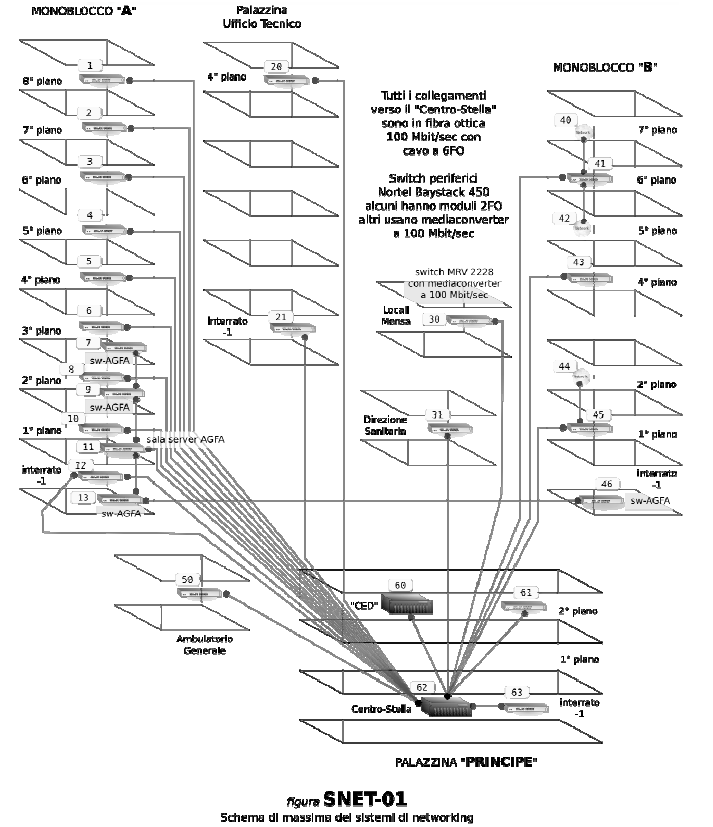
\includegraphics[scale=1]{./img/rete.png}
		\caption{Infrastruttura di rete della sede principale dell'istituto}
		\end{figure}
		Viene di seguito riportato l'elenco dettagliato delle apparecchiature di rete che costituiscono la LAN aziendale della sede principale. La tabella si riferisce alla figura precedente.
		\begin{longtable}{| c | c | p{6cm} |}
				\hline
				\textbf{Rif. figura} & \textbf{Sistema} & \textbf{Descrizione} \\ \hline
		1 & Armadio Rete & Nortel BayStack 450-24T \\ \hline
		2 & Armadio Rete & Nortel BayStack 450-24T \\ \hline
		3 & Armadio Rete & Nortel BayStack 450-24T \\ \hline
		4 & Armadio Rete & Nortel BayStack 450-24T \\ \hline
		5 & Armadio Rete & Nortel BayStack 450-24T \\ \hline
		6 & Armadio Rete & 2 x Nortel BayStack 450-24T \\ \hline
		7 & Armadio Rete & Nortel BayStack 450-24T (AGFA) \\ \hline
		8 & Armadio Rete & 2 x Nortel BayStack 450-24T e 2 x RackMediaConverter 12way (12+2 usate) \\ \hline
		9 & Armadio Rete & Nortel BayStack 450-24T (AGFA)\\ \hline
		10 & Armadio Rete & Cisco Catalyst 24pT \\ \hline
		11 & Armadio Rete & Cisco Catalyst 12pT \\ \hline
		12 & Armadio Rete & Cisco Catalyst 48pT + Cisco Catalyst 24pT \\ \hline
		13 & Armadio Rete & Nortel BayStack 450-24T (AGFA)\\ \hline
		20 & Armadio Rete & 3 x Nortel BayStack 450-24T \\ \hline
		21 & Armadio Rete & 4 x Nortel BayStack 450-24T \\ \hline
		30 & / & 2 x MRV 2228 + media converter \\ \hline
		31 & Armadio Rete & 4 x Nortel BayStack 450-24T \\ \hline
		40 & \textit{Cablaggio} & \textit{Servito da Armadio di Rete al sesto piano (41)} \\ \hline
		41 & Armadio Rete & 2 x Nortel BayStack 450-24T \\ \hline
		42 & \textit{Cablaggio} & \textit{Servito da Armadio di Rete al sesto piano (41)} \\ \hline
		43 & Armadio Rete & Nortel BayStack 450-24T + Catalyst 2950 \\ \hline
		44 & \textit{Cablaggio} & \textit{Servito da Armadio di Rete al primo piano (45)} \\ \hline
		45 & Armadio Rete & Nortel BayStack 450-24T + Nortel BayStack 151 (10BaseT) \\ \hline
		46 & / & 2 x Cisco Catalyst (24pT + 16 pT) \\ \hline
		50 & / & Cisco Catalyst 4506 \\ \hline
		60 & / & Cisco Catalyst 4510R \\ \hline
		61 & Armadio Rete & Synoptics-LattiHub-2814 + 3 x Nortel BayStack 450-24T + Media converter + UPS-Compaq \\ \hline
		62 & Armadio Rete & Centro-Stella \\ \hline
		63 & Armadio Rete & 3 x Nortel BayStack 450-24T \\ \hline
		\caption{Apparecchiature di rete della sede principale dell'istituto}
		\end{longtable}
	
	
	
		\myparagraph{Sicurezza}\\
		\\Dal punto di vista della sicurezza degli accessi da e verso Internet sono presenti due firewall e un proxy (ISA Server 2004).
		\newpage
		\subsubsection{Sede secondaria}
		
		Viene di seguito riportata una figura che illustra l'infrastruttura di rete della sede secondaria dell'istituto. Essa consta di un centro-stella connesso ai vari piani della struttura.
		\begin{figure}[h]
		\centering
		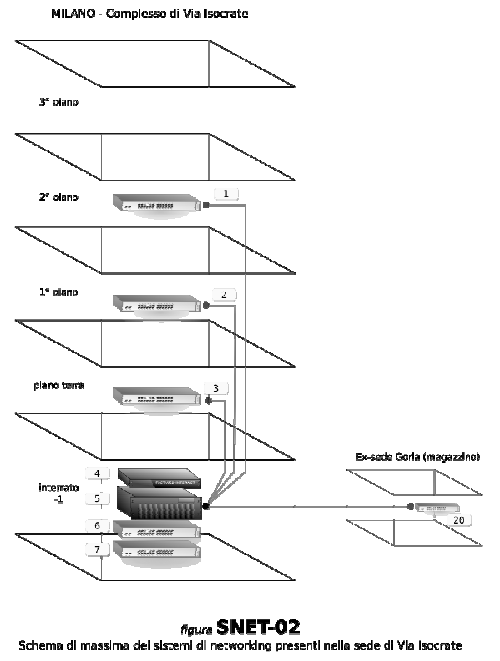
\includegraphics[scale=1]{./img/rete2.png}
		\caption{Infrastruttura di rete della sede secondaria dell'istituto}
		\end{figure}
		
		Viene di seguito riportato l'elenco dettagliato delle apparecchiature di rete che costituiscono la LAN aziendale della sede secondaria. La tabella si riferisce alla figura precedente.
		
		\begin{longtable}{| c | c | p{6cm} |}
				\hline
				\textbf{Rif. figura} & \textbf{Sistema} & \textbf{Descrizione} \\ \hline
				1 & Armadio Rete & Cisco Catalyst 2950 (24pT)\\ \hline
				2 & Armadio Rete & Cisco Catalyst 2950 (24pT)\\ \hline
				3 & Armadio Rete & 2 x Cisco Catalyst 2950 (24pT) + Cisco Catalyst 3560G (24pT) FUJI\\ \hline
				4 & Rack Rete & FASTWEB - Connessione Internet\\ \hline
				5 & Rack Rete & Cisco Catalyst 4510R (36pT)\\ \hline
				6 & Rack Rete & 2 x Cisco Catalyst 3560G (24pT) FUJI\\ \hline
				7 & Rack Rete & 2 x Cisco Catalyst 2911 (Rete Office + Rete Servizi)\\ \hline
				20 & Armadio Rete & Nortel BayStack 450-24T\\ \hline
				\caption{Apparecchiature di rete della sede secondaria dell'istituto}
		\end{longtable}
		
		\subsection{Hardware} \label{hardware}
		
		In questa sezione vengono presentate le apparecchiature hardware utilizzate dall'istituto per svolgere le attività quotidiane, ossia per offrire servizi ai pazienti.
		\subsubsection{Server}
		\myparagraph{Server primari}
		
		\begin{itemize}
			\item \textbf{Applicazione RAP (RCK-03)}: consiste di due sistemi SGI Origin200, interconnessi con il software FailSafe per garantirne l'alta affidabilità, sui quali è installato il software Agent di Oracle e di NFS. Il database è contenuto sui dischi dei due origin vault configurati ciascuno con 8 dischi in mirror tra di loro;
			\item \textbf{Disaster Recovery (RCK-07)}: consiste in due sistemi gemelli ai DB server (descritti successivamente) utilizzati inizialmente per effettuare test di Disaster/Recovery ma poi dismessi per altro utilizzo;
			\item \textbf{Test (RCK-06)}: consiste in un server SGI Origin 350 utilizzato per effettuare prove di migrazione e/o cambio configurazione del database. Attualmente dismesso per altro utilizzo.
		\end{itemize}
		
		\myparagraph{Server primari in comodato d'uso dal SISS}
		
		\begin{itemize}
			\item \textbf{DB Server (RCK-06)}: comprende due sistemi SGI Altix350, ciascuno con 2 processori Mips R16k a 800MHz e 16 GB di memoria, con doppio alimentatore ridondato e uno storage della famiglia InfiniteStorage modello TP9300 con 14 dischi da 146GB SCSI, per una capacità totale di 2TB raw, ed interconnessione in FiberChannel a 2Gbit per una bandwidth complessiva fino a 800Mbytes/sec.
			Su questi server è installato il DB Oracle versioni 9i e 10g Enterprise (4 processori) in
			modalità RACK su cui sono memorizzati i dati dei seguenti applicativi: Aurora Web (PS, ADT, CUP), GST (Casse), Powerlab (Lab. Analisi), Aliseo (gestione personale), Enco (amministrazione);
			\item \textbf{Application Server (Siemens - Aurora - RCK-01)}: sistema composto da due server (HP DL380 con storage condiviso HP MSA 1000 con 8 HD da 72GB) con SO Linux (RedHat Enterprise v.3 upd. 6), identici dal punto di vista hardware e software, in cui però i servizi realmente attivi sono suddivisi tra le due macchine.
			Il Cluster SIEMENS ha l'obiettivo di erogare applicazioni web utilizzando l'Application Server IBM WebSphere;
			\item \textbf{Application Server (Santer - repository, middleware, BDA - RCK-01)}: il sistema è identico al precedente. Sul cluster Santer è installata la ``soluzione regionale" che comprende il software di base per repository, middleware ICan e la BDA (Banca Dati Anagrafiche). L'application server è basato su Apache Tomcat;
			\item \textbf{Porta applicativa SISS}: comprende server, routers, firewall e software necessari alla gestione delle connessioni dall'esterno da parte dei medici di medicina generale (MMG) e/o medici di altre AO per la visualizzazione dei referti memorizzati sul repository locale. La porta applicativa, fisicamente identificata da un unico rack presso il centro stella, è a totale gestione di Lisit.
		\end{itemize}
		
		\myparagraph{Altri Server}
		
		\begin{itemize}
			\item \textbf{Gestione archiviazione cartelle cliniche cartacee}: gestisce la identificazione e localizzazione delle cartelle cliniche cartacee presenti presso l'archivio cartelle cliniche;
			\item \textbf{Server RIS/PACS}: apparecchiature specifiche (server e storage) per il funzionamento del sistema RIS/PACS fornito dall'AGFA.
		\end{itemize}
		
		\myparagraph{Situazione server}\\
		\\Viene riportata una figura che visualizza le apparecchiature e i server presenti nella sala macchina presso il CED dell'istituto.
		
		\begin{figure}[h]
		\centering
		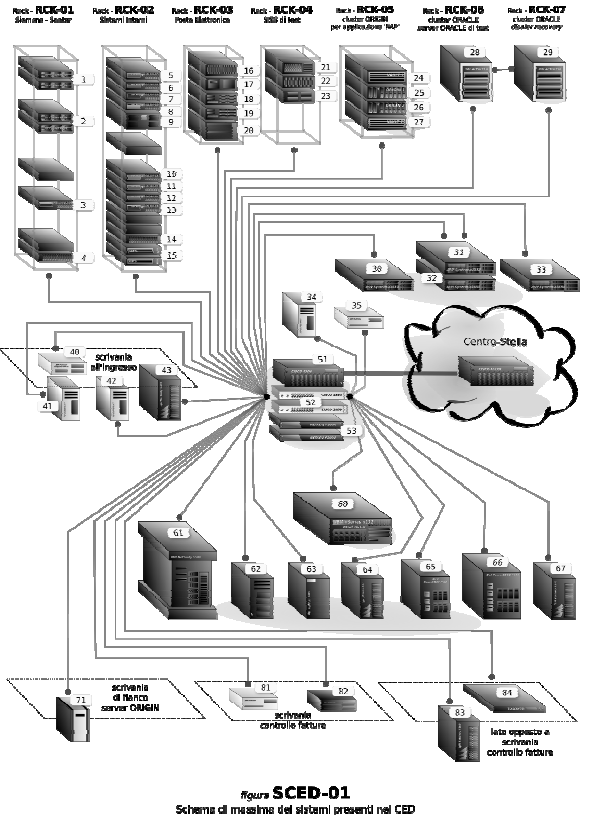
\includegraphics[scale=1]{./img/server.png}
		\caption{Situazione server dell'istituto}
		\end{figure}
		\newpage
		Viene di seguito riportato l'elenco dettagliato delle apparecchiature hardware che fanno parte dell'istituto. La tabella si riferisce alla figura precedente.
		\begin{longtable}{| c | c | p{6cm} |}
				\hline
				\textbf{Rif. figura} & \textbf{Sistema} & \textbf{Descrizione} \\ \hline
				1 & SANTER{1,2} & Application Server (Cluster) SANTER con applicazioni: BDA, SISSWAY, REPOSITORY \\ \hline
				2 & SIEMENS{1,2} & Application Server (Cluster) SIEMENS con applicazione AURORAWEB \\ \hline
				3 & HP SAN & Storage utilizzato dalle applicazioni presenti nel rack \\ \hline
				4 & HP SAN & Storage utilizzato dalle applicazioni presenti nel rack  \\ \hline
				5 & MARCONI & Replica DFS (Distibuted File System di Microsoft) \\ \hline
				6 & DAFNE & Applicazione INTRANET \\ \hline
				7 & PITAGORA & Applicazioni: PRESENZE, ARCHIVIO CLINICO \\ \hline
				8 & / & Applicazione (portale) INTERNET \\ \hline
				9 & HP TAPE LIBRARY & HP Tape Library per utilizzo con backup server (11) \\ \hline
				10 & NEWTON & Applicazione: Oracle Grid Console \\ \hline
				11 & EDISON & Applicazione: Backup (9) \\ \hline
				12 & ARCHIMEDE & Primo server del cluster Microsoft Exchange 2007 \\ \hline
				13 & VOLTA & Secondo server del cluster Microsoft Exchange 2007 \\ \hline
				14 & HP STGWORKS & SAN del rack \\ \hline
				15 & APC UPS & Gruppi di continuità del rack \\ \hline
				16 & IBM STORAGE & SAN del rack \\ \hline
				17 & IBM TAPE LIBRARY & Tape Library del rack \\ \hline
				18 & ERA (1) & Server Microsoft Windows 2003 con Micorosft
Exchange 2003 (posta elettronica) \\ \hline
				19 & ERA (2) & Server Microsoft Windows 2003 con servizi DFS,
DHCP, WINS e DNS \\ \hline
				20 & APC UPS & Gruppo di continuità del rack \\ \hline
				21 & SISS-TEST & Server SISS di test \\ \hline
				22 & IBM STORAGE & SAN del rack \\ \hline
				23 & IBM TAPE LIBRARY & Tape Library del rack \\ \hline
				24 & VAULT1 & Tape Library del rack (applicazione RAP) \\ \hline
				25 & ORIGIN1 & Applicazione RAP \\ \hline
				26 & ORIGIN2 & Applicazione RAP \\ \hline
				27 & VAULT2 & Tape Library del rack (Applicazione RAP) \\ \hline
				28 & ORACLE+TEST & Consolidamento database Oracle \\ \hline
				29 & ORACLE-D.R. & Consolidamento database Oracle (Disaster Recovery) \\ \hline
				30 & / & Applicazione: Asset Management con Microsoft SMS \\ \hline
				31 & MINERVA & Controllore di dominio \\ \hline
				32 & ATHENA & Accesso remoto \\ \hline
				33 & / & Proxy Server \\ \hline
				34 & SISSTEST1 & Controllo timbrature della mensa (pagamento pasto) \\ \hline
				35 & CONCENTRATORE ZUCCHETTI & Concentratore Zucchetti, gestione timbrature \\ \hline
				40 & OPN & Grouper (Valorizzazione DRG regionali) \\ \hline 
				41 & / & Server video sorveglianza \\ \hline
				42 & POLLING & Applicazione di polling per Siemens/GST \\ \hline
				43 & FWUNIMI & Firewall Università di Milano \\ \hline
				51 & ROUTER CISCO & Router Cisco della sala CED \\ \hline
				52 & SWITCH & Switch di distribuzione rete della sala CED \\ \hline
				53 & 2 x NETASQ F1000 & Firewall aziendale \\ \hline
				60 & PROTOCOLLO & Applicazione: Protocollo BETA80 \\ \hline
				61 & (dismesso) & Smantellamento e recupero parti da riutilizzare su altri server \\ \hline
				62 & PROXY ISOCRATE & Proxy per Via Isocrate \\ \hline
				63 & ORMA & Vecchia versione di Oracle \\ \hline
				64 & SCRIBA & Printer Server \\ \hline
				65 & HORUS & Connessioni remote con virtualizzazione di sistemi Windows XP \\ \hline
				66 & ARGOS & Applicazione: TESEO \\ \hline
				67 & DWH & Applicazioni: DWH e Archivio Clinico \\ \hline
				71 & AURORA & Siemens - Test applicazione AURORAWEB \\ \hline
				81 & IOGP & Monitoring RAP e Punti Gialli \\ \hline
				82 & PCMENSA & Monitoring RAP \\ \hline
				83 & PRESENZE & Applicazione: Presenze NHR \\ \hline
				84 & / & Server utilizzato per test vari \\ \hline
				\caption{Apparecchiature hardware dell'istituto}
		\end{longtable}
		
		
		
		\subsubsection{Terminali per la rilevazione delle presenze}
		
		L'istituto presenta tredici terminali Zucchetti dedicati alla rilevazione delle presente e al controllo degli accessi. La seguente tabella illustra la posizione dei terminali e il loro modello.
		\newpage
		\begin{longtable}{| c | c | c |}
		\hline
		\textbf{Sede} & \textbf{Posizione} & \textbf{Modello}\\ \hline
		Principale & Padiglione principale & 2 x GONG P2 M \\ \hline
		Principale & Direzione sanitaria & GONG P2 M \\ \hline
		Principale & Palazzina mensa & 2 x GONG P3 M \\ \hline
		Secondaria & Ingresso & GONG P3 M \\ \hline
		Secondaria & Ambulatorio & GONG P3 M \\ \hline
		Secondaria & Mensa & GONG P3 M \\ \hline
		Principale & Santa Sofia blocco A P.8 & 2 x GONG P2 M \\ \hline
		Principale & Corridoio Alpa & GONG P2 M \\ \hline
		Principale & Blocco operatorio & UGONGT3NM + GONG TA M \\ \hline
		\caption{Terminali per la rilevazione delle presenze dell'istituto}
		\end{longtable}
		
		\subsubsection{Postazioni di lavoro}
	
		L'istituto presenta postazioni di lavoro di differente annata. Le ultime acquisizioni provengono dai progetti regionali. La manutenzione delle postazioni di lavoro è a carico di Lombardia Informatica.
		Le postazioni inventariate sono 486. Il numero è destinato ad incrementarsi per l'arrivo di nuove postazioni già immagazzinate. Nella seguente tabella viene riportata la lista delle postazioni di lavoro suddivisa per modello e per anno di installazione.
		
		\begin{longtable}{| c | c | c |}
		\hline
		\textbf{Modello} & \textbf{Quantità} & \textbf{Anno}\\ \hline
		Sconosciuto & 47 & Sconosciuto \\ \hline
		Sconosciuto & 1 & 1994 \\ \hline
		ELI 40035-Z & 1 & 1995 \\ \hline
		R4400SC & 1 & 1996 \\ \hline
		VECTRA VE 5 & 1 & 1997 \\ \hline
		CWP 50033 & 1 & 1997 \\ \hline
		Sconosciuto & 2 & 1998 \\ \hline
		EP PII & 2 & 1999 \\ \hline
		IBM & 1 & 1999 \\ \hline
		OMEGA PC PII & 1 & 1999 \\ \hline
		DESKPRO EN 6350 & 1 & 1999 \\ \hline
		6563-W6G & 12 & 2000 \\ \hline
		DP EP PIII500 & 1 & 2000 \\ \hline
		EP PIII500 & 16 & 2000 \\ \hline
		Sconosciuto & 1 & 2000 \\ \hline
		PC300GL & 30 & 2000 \\ \hline
		7100 & 1 & 2000 \\ \hline
		Sconosciuto & 2 & 2001 \\ \hline
		HP 970C DESKJET & 1 & 2001 \\ \hline
		A22P & 1 & 2002 \\ \hline
		A22P DT & 12 & 2002 \\ \hline
		A22P DT P4 & 1 & 2002 \\ \hline
		A22P P4 & 1 & 2002 \\ \hline
		CASE MINI TOWER ATX & 1 & 2002 \\ \hline
		N4ETVISTA A22P & 1 & 2002 \\ \hline
		Sconosciuto & 2 & 2002 \\ \hline
		NETRVISTA A22P & 1 & 2002 \\ \hline
		NETVISTA A22P & 4 & 2002 \\ \hline
		A22P P4 & 1 & 2002 \\ \hline
		SATELLITE 1800-514 & 1 & 2002 \\ \hline
		P4 6349-74G & 1 & 2002 \\ \hline
		P4 6791 11G & 1 & 2002 \\ \hline
		IBM P4 TYPE 8609 & 1 & 2002 \\ \hline
		D SAMARA & 1 & 2003 \\ \hline
		COMPAQ HP & 1 & 2003 \\ \hline
		COMPAQ/HP EVO & 2 & 2003 \\ \hline
		ED SAMARA & 15 & 2003 \\ \hline
		Sconosciuto & 4 & 2003 \\ \hline
		P4 A30P TYPE8309 & 1 & 2003 \\ \hline
		TS A30P TYPE8309 & 2 & 2003 \\ \hline
		VTPF2 & 1 & 2003 \\ \hline
		CDS THOR P4VE-2.5GHZ & 1 & 2003 \\ \hline
		IBM TS A30P 8309 & 1 & 2003 \\ \hline
		P4 TYPE 8309 & 1 & 2003 \\ \hline
		TS A30P TYPE8309 & 1 & 2003 \\ \hline
		D530 & 1 & 2004 \\ \hline
		D530 P4 & 1 & 2004 \\ \hline
		D530 P4 & 1 & 2004 \\ \hline
		ACER POWER M2 & 1 & 2004 \\ \hline
		DS30 & 1 & 2004 \\ \hline
		ML350T G3 & 1 & 2004 \\ \hline
		P4 RAM256 MB & 1 & 2004 \\ \hline
		TYPE 6269-V56 & 1 & 2004 \\ \hline
		ACER POWER M2 & 14 & 2004 \\ \hline
		BOM IT 34 & 1 & 2004 \\ \hline
		DT P4 2.66 & 1 & 2004 \\ \hline
		P4 RAM 256 MB & 14 & 2004 \\ \hline
		P4 2,8 256 MB & 1 & 2004 \\ \hline
		IBM 300 GL & 1 & 2004 \\ \hline
		HP DX 2000 MT P4 2,8 & 3 & 2004 \\ \hline
		PIII A20 6269 P7G & 1 & 2004 \\ \hline
		PIII A20 6269 V5G & 9 & 2004 \\ \hline
		PIII A20 TPE 6269 & 1 & 2004 \\ \hline
		PIII A20 TYPE 6269 & 13 & 2004 \\ \hline
		PIII A20 TYPTE 6269 & 1 & 2004 \\ \hline
		PIII800 6269 P7G & 1 & 2004 \\ \hline
		BUSINESS DESKTOP DC7 & 1 & 2005 \\ \hline
		HP BUSINESS DESKTOP & 1 & 2005 \\ \hline
		HP DX2000 & 2 & 2005 \\ \hline
		HP DX2000 P4 & 1 & 2005 \\ \hline
		HP PAVILLON RMIN73 & 1 & 2005 \\ \hline
		HP PAVILLON RMIN74 & 1 & 2005 \\ \hline
		Sconosciuto & 1 & 2005 \\ \hline
		SG FLYER & 3 & 2005 \\ \hline
		P4 512 MB con master & 1 & 2005 \\ \hline
		DX2000 P4 & 1 & 2005 \\ \hline
		P4 DC 5100 & 1 & 2005 \\ \hline
		DX 5150 P4 & 36 & 2005 \\ \hline
		DX2000 P4 & 7 & 2006 \\ \hline
		DX2000 P4 WXP & 1 & 2006 \\ \hline
		DX5150 MT & 1 & 2006 \\ \hline
		DX5150 MT XPP & 1 & 2006 \\ \hline
		HP DX5150 & 2 &  2006\\ \hline
		Sconosciuto & 28 & 2006 \\ \hline
		MT-M8296-714 & 1 & 2006 \\ \hline
		LCD 17' L1702 & 1 & 2006 \\ \hline
		MT-M 8296-714 & 2 & 2006 \\ \hline
		GX280 P4530 & 1 & 2007 \\ \hline
		Sconosciuto & 15 & 2007 \\ \hline
		P4530 & 1 & 2007 \\ \hline
		P4-530 & 3 & 2007 \\ \hline
		DX5150 SFF AX-2 & 1 & 2007 \\ \hline
		P4 530 & 33 & 2007 \\ \hline
		HP DX5150MT (SISS) & 37 & 2008 \\ \hline
		DX 5150 (SISS) & 16 & 2008 \\ \hline
		DX 5150MT (SISS) & 33 & 2008 \\ \hline
		\caption{Postazioni di lavoro dell'istituto}
		\end{longtable}

	
	\subsection{Software} \label{software}
	
	In questa sezione vengono illustrati i software utilizzati dall'istituto per:
	\begin{itemize}
		\item L'erogazione di servizi sanitari e amministrativi;
		\item La gestione dei sistemi sanitari e amministrativi;
		\item L'utilizzo delle postazioni di lavoro.
	\end{itemize}
	
	\subsubsection{Software per erogazione di servizi}
	
	Nella seguente tabella vengono riportate le applicazioni per l'erogazione dei servizi dell'istituto, con la relativa descrizione.
	\begin{longtable}{| c | p{10cm} |}
		\hline
		\textbf{Applicazione} & \textbf{Descrizione}\\ \hline
		Gestione dei punti gialli & Applicazione che gestisce il pagamento dei ticket da parte degli utenti dell'istituto\\ \hline
		Gestione fatture & Applicazione che gestisce la fatturazione SSN e la fatturazione dei medici che esercitano in regime di `intromoenia' \\ \hline
		Valorizzazione ricoveri & Applicazione per la verifica e la valorizzazione dei ricoveri \\ \hline
		Gestione pazienti in urgenza & Applicazione per la gestione del Pronto Soccorso \\ \hline
		Piattaforma SISS & Applicazione che permette di accedere ai sistemi e servizi forniti dal progetto regionale SISS \\ \hline
		Gestione archivio clinico & Applicazione per la gestione dell'archiviazione delle cartelle cliniche cartacee \\ \hline
		Gestione produzione emoderivati & Applicazione che gestisce le sacche di sangue \\ \hline
		Gestione pazienti & Applicazione per la gestione del paziente in regime ambulatoriale e degenza \\ \hline
		Gestione diagnostica per immagini & Applicazione per la gestione di immagini digitali radiologiche e refertazione \\ \hline
		Gestione anatomia patologica & Applicazione per la gestione dei referti \\ \hline
		Gestione sale operatorie & Applicazione per la gestione della lista e del verbale operatorio \\ \hline
		Gestione del materiale protesico & Applicazione per la gestione delle protesi utilizzate durante gli interventi chirurgici \\ \hline
		Gestione laboratorio analisi & Applicazione per la gestione degli strumenti e della refertazione delle prestazioni di laboratorio \\ \hline
		Gestione delle risorse umane & Applicazione per la gestione integrata delle risorse umane dell'istituto \\ \hline
		Gestione protocollo & Applicazione per la gestione del protocollo generale \\ \hline
		Gestione amministrazione e magazzini & Applicazione per la gestione integrata della contabilità. dei magazzini economali e della farmacia \\ \hline
		\caption{Software per l'erogazione dei servizi IT}
	\end{longtable}
	
	
	\subsubsection{Software per la gestione dei sistemi}
	
	Viene di seguito fornita una descrizione degli applicativi utilizzati per la gestione delle attività sanitarie primarie:
	
	\begin{itemize}
		\item \textbf{GST Esterni e Aurora Web}: per la gestione dei pazienti ricoverati sono state introdotte nuove applicazioni della linea di prodotto Aurora Web al fine di consentire di gestire in modo semplificato la distribuzione dell'applicazione e il decentramento organizzativo. Dato l'elevato livello d'integrazione esistente tra la gestione dei ricoveri ed il Pronto Soccorso, anche per quest'ultimo è stato previsto un percorso di evoluzione tecnologica che ha comportato la migrazione all'applicativo Aurora Web.
		Per l'ambito applicativo inerente il trattamento dei pazienti ambulatoriali, si è ritenuto opportuno, invece, non sostituire il software che rimane in modalità client/server, data la forte personalizzazione del software stesso (Siemens GST ESTERNI). Anche per il trattamento dei pazienti interni e del Servizio di Traumatologia d'Urgenza è stato introdotto l'applicativo Aurora web;
		\item \textbf{Powerlab}: applicativo di tipo client/server interfacciato con gli strumenti di laboratorio e già integrato al SISS. In particolare sono attive le funzioni che consentono di firmare digitalmente il referto per l'invio dello stesso al repository centrale nelle varie modalità previste da progetto. Le funzioni di acquisizione di una richiesta di prestazione da parte di ambulatori, reparto e Pronto Soccorso sono state sviluppate ma non attivate;
		\item \textbf{Radiologia}: presso la sede centrale il fornitore del RIS è Agfa (applicativo RIS Elefante). L'applicativo è integrato al PACS per la gestione integrata delle immagini digitali radiologiche e relativo referto ed è già integrato al SISS. In particolare sono attive le funzioni che consentono: 
			\begin{enumerate}
			\item l'acquisizione di una richiesta di prestazione da parte di: casse, reparto e
			Pronto Soccorso;
			\item  gestire lo stato della prestazione;
			\item firmare digitalmente il referto
			per l'invio dello stesso al repository centrale nelle varie modalità previste da progetto.
			\end{enumerate}
		Presso la sede di Via Isocrate è stata realizzata una seconda rete radiologica con RIS fornito da AGFA e sistema PACS fornito da Fuji;
		\item \textbf{Armonia}: applicativo client/server non ancora integrato al SISS;
		\item \textbf{Emonet}: applicativo client/server richiesto da Regione Lombardia per la gestione delle sacche di plasma. È prevista l'integrazione con la Fondazione Policlinico, che fornirà quindi il servizio applicativo da remoto, e relativa migrazione della base dati. Non è prevista alcuna integrazione al SISS;
		\item \textbf{ORMAWIN2000}: l'applicazione è utilizzata in particolare per la gestione dei verbali operatori e delle endoprotesi che rappresentano una voce considerevole dei costi di esercizio della chirurgia. Tramite software terzi ed attività manuale i dati sono riversati all'interno dell'applicativo amministrativo (Enco).
	\end{itemize}
	Viene di seguito fornita una descrizione degli applicativi utilizzati per la gestione delle attività amministrative primarie:
	
	\begin{itemize}
		\item \textbf{Enco}: applicativo per la gestione della contabilità generale ed analitica, dei magazzini economali e farmacia. Per la fatturazione attiva delle prestazioni e l'incasso (casse CUP e Spedalità) è utilizzato il sistema sanitario che trasmette i dati al sistema di contabilità. Un modulo a parte si occupa del calcolo delle spettanze per le attività di libera professione e inserisce nel sistema di contabilità le relative scritture. La gestione di
		magazzino farmaceutico è centralizzata, non sono cioè attive postazioni per la gestione di armadietti di reparto. La gestione della apparecchiature elettromedicali (acquisizione, manutenzione, rapporti con le aziende di ingegneria clinica) è di competenza dell’Ufficio Tecnico ma i dati di interesse economico-contabile devono essere inseriti anche nel sistema amministrativo. La gestione dei costi del materiale protesico è molto importante per l'istituto ma attualmente è effettuata con un modulo esterno al sistema amministrativo contabile;
		\item \textbf{Aliseo}: applicativo per la gestione giuridica, delle presenze e cedolini paghe.
		Al momento gran parte delle attività sono eseguite internamente da personale afferente alla UO Personale. La rete del sistema di rilevazione presenze è di un fornitore diverso (Zucchetti). Il sistema è integrato alla contabilità. L'applicativo è in architettura client/server anche se prevede l'utilizzo di interfacce web per funzioni da distribuire agli utenti, non attive presso l'istituto.
	\end{itemize}
	
	\subsubsection{Software installato sulle postazioni di lavoro}
	
	Il software installato su una postazione di lavoro è:
	\begin{itemize}
		\item Sistema operativo Windows XP Sp2;
		\item Antivirus eTrust V. 7.1;
		\item SISS v. 9.x.x per la connessione al SISS;
		\item Sissway (client del repository) per la connessione alla BDA e la firma digitale;
		\item MS Office.
	\end{itemize}
	\newpage
	\subsubsection{Middleware di integrazione}
	
	Una componente fondamentale del sistema informativo dell'istituto consiste in un middleware di integrazione fornito, nell'ambito del progetto SISS, da Regione Lombardia. Tale soluzione, realizzata dalla ditta Santer, comprende:
	\begin{itemize}
		\item \textbf{Database anagrafiche centralizzato}: contiene tutte le anagrafiche dei cittadini lombardi ed a cui tutti gli applicativi devono interfacciarsi per l'acquisizione di una anagrafica esistente o la validazione di una nuova anagrafica;
		\item \textbf{Repository referti}:  a cui i singoli applicativi inviano il referto firmato digitalmente, al momento in formato PDF, a cui viene attribuito un codice univoco e memorizzato sul DB dello stesso repository. Sono presenti funzioni per la marcatura temporale e l'invio del link ai domini centrali SISS, previa verifica dell'avvenuta registrazione del pagamento della prestazione effettuata.
	\end{itemize}
	
	\newpage
	
	\section{Personale} \label{personale}
	
	Il CPC deve designare i team per implementare la strategia di ripristino del sistema. Ogni team deve essere addestrato e pronto ad intervenire in caso si verifichi una situazione che richiede l'attivazione del piano.
	Il personale di recupero deve essere assegnato ad uno dei vari team specifici che risponderanno all'evento, recupereranno le funzionalità e restituiranno il sistema alle normali operazioni. Per fare ciò, il personale deve comprendere chiaramente l'obiettivo del team in ogni fase da eseguire durante il ripristino e in che modo il team si relaziona con gli altri team.\\
	I team preposti includono il personale responsabile delle operazioni giornaliere e sono basati sul sistema interessato. Le azioni e la dimensione di ognuno di essi dipendono dall'organizzazione.
	
	\subsection{Ordine di successione}
	
	L'istituto stabilisce un ordine di successione in coordinamento con l'ordine stabilito dal dipartimento, per garantire che l'autorità decisionale per il piano di emergenza dell'istituto sia ininterrotta. Il Chief Information Officer (CIO) dell'istituto ha la responsabilità di garantire la sicurezza del personale e l'esecuzione delle procedure documentate all'interno di questo piano. Se il CIO non è in grado di funzionare come autorità generale o sceglie di delegare questa responsabilità a un successore, il vice CIO fungerà da tale autorità.
	
		\subsection{Team preposti}			
		
		In questa sezione sono riportati i team che verranno assegnati nell'esecuzione del piano di contingenza.
		
			\subsubsection{Senior Management Official}
			Il Senior Management Official è responsabile della gestione esecutiva di tutti gli aspetti del piano di contingenza. Le sue responsabilità sono le seguenti:
			\begin{itemize}
				\item Pre-evento
					\begin{itemize}
						\item Approva il piano;
						\item Assicura che sia mantenuto;
						\item Assicura che venga condotto l'addestramento;
						\item Autorizza test periodici del piano.
					\end{itemize}
				\item Post-evento
					\begin{itemize}
						\item Dichiarazione del disastro;
						\item Autorizza le modalità di viaggio e alloggio per i membri del team;
						\item Autorizza le spese attraverso il team amministrativo;
						\item Gestisce e monitora il processo di recupero complessivo;
						\item Informa periodicamente il personale senior, i clienti e il personale addetto alle relazioni con i media dello stato;
						\item Supporta il Contingency Management Team durante situazioni debilitanti.
					\end{itemize}
			\end{itemize}
			
			\subsubsection{Contingency Management Team}
			Il team di gestione della contingenza è responsabile della gestione del ripristino per garantire che altri team e personale eseguano tutte le voci della checklist e fornire un centro per il coordinamento e le comunicazioni generali. Inoltre, garantisce che le attività siano svolte tra tutte le squadre entro i tempi previsti e fornisce assistenza nella risoluzione dei problemi che possono sorgere. Questo team è attivato dal Senior Management Official o dal proprietario del sistema. Tutti gli altri team riferiscono direttamente al presente team.
				\myparagraph{Contingency Management Team Leader}\\
				\\Le sue responsabilità sono le seguenti:
				\begin{itemize}
					\item Pre-evento
					\begin{itemize}
						\item Mantiene e aggiorna il piano secondo necessità ma non meno di una volta all'anno;
						\item Distribuisce il piano ai membri del team;
						\item Coordina i test secondo necessità ma non meno di una volta all'anno;
						\item Addestra i membri del team.
					\end{itemize}
					\item Post-evento
						\begin{itemize}
							\item Compila la notifica iniziale dei membri del team;
							\item Stabilisce un centro di comando per le operazioni di ripristino;
							\item Assiste nella valutazione del danno;
							\item Coordina le attività dei team di recupero;
							\item Notifica di attivazione del sito alternativo;
							\item Avvisa i leader di altri team dell'attivazione del piano;
							\item Autorizza il team amministrativo a programmare i viaggi e le sistemazioni alberghiere necessarie per i membri del team di recupero;
							\item Riferisce periodicamente lo stato del ripristino e i dettagli richiesi al Senior Management Official.
						\end{itemize}
				\end{itemize}
				\myparagraph{Contingency Management Team Members}\\
				\\Le responsabilità dei membri sono le seguenti:
				\begin{itemize}
					\item Pre-evento
					\begin{itemize}
						\item Assistono il leader del team;
						\item Partecipano all'addestramento e ai test di contingenza;
						\item Comprendono tutti i ruoli e le responsabilità del piano di contingenza.
					\end{itemize}
					\item Post-evento
					\begin{itemize}
						\item Eseguono le funzioni del centro di comando/coordinamento;
						\item Mantengono una registrazione di tutte le comunicazioni, utilizzando i moduli di registro forniti.
					\end{itemize}
				\end{itemize}
			
			Il Management Team è una parte essenziale del business, in quanto ne analizza ed identifica gli obiettivi per implementare una strategia di successo.  
			Questo team gestisce e controlla le attività di ripristino che si svolgono durante l'esecuzione del piano di contingenza.
			
			\subsubsection{Damage Assessment Team}
			Il Damage Assessment Team è un gruppo tecnico responsabile della valutazione dei danni al sistema e ai suoi componenti. Il team inizia ad operare in seguito all'attivazione del piano. È composto da personale con una conoscenza approfondita dell'hardware e delle attrezzature. Questo team è il principale responsabile della valutazione iniziale del danno, della minimizzazione delle perdite, del salvataggio e dell'approvvigionamento delle attrezzature sostitutive necessarie.
			Il team diventa operativo dal momento in cui riceve l'autorizzazione ad entrare nella struttura dai servizi di emergenza. Inoltre, il team deve redarre un resoconto dettagliato dello stato generale del sistema, con particolare attenzione alle condizioni di hardware, software, arredi e infissi. È necessario che tutte le attrezzature e i supporti danneggiati con annessa documentazione siano indirizzati immediatamente al Contingency Management Team. Le responsabilità sono:
			\begin{itemize}
				\item Pre-evento
				\begin{itemize}
					\item Comprende il ruolo e le responsabilità sotto il piano di contingenza;
					\item Cerca di ridurre la probabilità di eventi che potrebbero richiedere l'attivazione del piano;
					\item Addestra i dipendenti in caso di emergenza;
					\item Partecipa alle esercitazioni e test del piano di contingenza;
					\item Ha una conoscenza approfondita delle procedure di valutazione dei danni.
				\end{itemize}
				\item Post-evento
				\begin{itemize}
					\item Determina l'accessibilità a strutture, edifici, uffici e aree di lavoro;
					\item Valuta l'entità del danno al sistema e ai suoi componenti;
					\item Valuta la necessità e/o l'adeguatezza della sicurezza;
					\item Stima il tempo necessario per ripristinare la struttura e il sistema primario;
					\item Identifica l'hardware recuperabile;
					\item Informa il Contingency Management Team circa l'entità dei danni, i tempi di recupero stimati, la necessità di sicurezza fisica e i dettagli delle attrezzature recuperabili;
					\item Mantiene un registro delle attrezzature salvabili;
					\item Coordina i fornitori del ripristino, la riparazione o la sostituzione di apparecchiature non sotto la responsabilità di un altro piano;
					\item Supporta la pulizia del CED in seguito ad un incidente.
				\end{itemize}
			\end{itemize}		
			
			\subsubsection{Hardware Team}
			L'Hardware Team è responsabile della preparazione del sito, della pianificazione fisica e dell'installazione delle apparecchiature di elaborazione dei dati per fornire la capacità di elaborazione richiesta quando il piano è attivato. Le responsabilità del team comprendono l'ordinazione e l'installazione di hardware e software necessari nei siti primari e alternativi.
			Le responsabilità del team sono le seguenti:
			\begin{itemize}
				\item Pre-evento
				\begin{itemize}
					\item Comprende i ruoli e le responsabilità sotto il piano di contingenza;
					\item Lavora a stretto contatto con il Contingency Management Team per ridurre la probabilità di eventi che potrebbero richiedere l'attivazione del CP;
					\item Addestra i dipendenti alle emergenze;
					\item Partecipa alle esercitazioni e ai test del piano;
					\item Comprende a fondo le procedure del piano;
					\item Mantiene le informazioni sulla configurazione del sistema corrente in una struttura di archiviazione esterna e in questo piano.
				\end{itemize}
				\item Post-evento
				\begin{itemize}
					\item Verifica i requisiti di occupazione in sospeso con un sito alternativo;
					\item Ispeziona lo spazio fisico nel sito alternativo;
					\item Si interfaccia con i membri del team Software, Comunicazioni e Operazioni sulla configurazione dello spazio per il sito alternativo;
					\item Coordina il trasporto di attrezzature recuperabili al sito alternativo;
					\item Notifica al team amministrativo i requisiti dell'apparecchiatura;
					\item Garantisce l'installazione dei terminali temporanei e delle workstation necessari collegati all'hardware del sito alternativo;
					\item Pianifica l'installazione dell'hardware sul sito alternativo;
					\item Pianifica e coordina il trasporto e l'installazione dell'hardware nel sito permanente, se disponibile.
				\end{itemize}
			\end{itemize}
			\myparagraph{Hardware Salvage Team}\\ 
			\\L'Hardware Salvage Team localizza e coordina la consegna e installazione di terminali utente, stampanti, macchine da scrivere, fotocopiatrici, e altre apparecchiature necessarie. Offre supporto al gruppo delle comunicazioni e a qualsiasi tentativo per il salvataggio di hardware e apparecchiature.
			
			\subsubsection{Software Team}
			Il Software Team è responsabile dell'installazione e della configurazione di tutti i software di sistema e delle applicazioni non installate da altri amministratori. Le responsabilità del team sono le seguenti:
			\begin{itemize}
				\item Pre-evento
				\begin{itemize}
					\item Comprende i ruoli e le responsabilità sotto il piano di contingenza;
					\item Lavora a stretto contatto con il Configuration Management Team per ridurre la probabilità di eventi che potrebbero richiedere l'attivazione del CP;
					\item Addestra i dipendenti in caso di emergenze;
					\item Partecipa a esercitazioni e test del piano;
					\item Comprende a fondo le procedure del piano;
					\item Mantiene aggiornate le informazioni sulla configurazione del software di sistema in una struttura di archiviazione esterna.
				\end{itemize}
				\item Post-evento
				\begin{itemize}
					\item Organizza la consegna di contenitori di stoccaggio fuori sede contenenti supporti di backup;
					\item Riceve, inserisce nell'inventario e controllare l'accesso ai contenitori e ai supporti di archiviazione fuori sede;
					\item Ripristina i file di dati del software di sistema e delle applicazioni non installate insieme ad un altro piano del personale;
					\item Testa e verifica le funzioni del sistema operativo e del software applicativo secondo necessità;
					\item Restituisce i contenitori di archiviazione dei supporti di backup nella struttura di archiviazione esterna.
				\end{itemize}
			\end{itemize}
			\myparagraph{Systems Software Team}\\
			\\È responsabile di effettuare il ``restore" dei dischi di sistema, di caricare e provare il software del sistema operativo, e di risolvere i problemi a livello sistemistico.
			Questo team è composto da programmatori software responsabili della fornitura del supporto software necessario per la produzione di applicazioni di sistema critiche durante il ripristino.
			
			\myparagraph{Server Recovery Team}\\
			\\È responsabile di tutte le attività sistemistiche ed operative per il ripristino dei server e server farm.
			
			
			\myparagraph{LAN Recovery Team}\\
			\\È responsabile del reinstradamento delle comunicazioni voce e dati su larga scala e del ristabilimento degli accessi alla rete presso il sito di recovery del sistema.
			
			\myparagraph{Database Recovery Team}\\
			\\Aggiorna i database applicativi lavorando da terminali installati presso il sito di recovery utente. Supervisiona il personale temporaneo addetto all'immissione dati e assiste ai tentativi di salvataggio dei record acquisendo i documenti originali e altre fonti d'informazione.
			
			
			\myparagraph{Application Recovery Team}\\
			\\Si reca al sito di recovery del sistema ed effettua il restore dei dischi utente e dei programmi applicativi sul sistema. Man mano che procede il recovery, questo gruppo può assumere la responsabilità di controllare le prestazioni applicative e l'integrità dei database.
			
			
			\myparagraph{Telecommunications Team}\\
			\\Si reca al sito di recovery utente dove lavora insieme con il gruppo di recovery delle reti remote per ristabilire una rete utente/sistema. È anche responsabile dell'installare hardware per le comunicazioni presso il sito di recovery utente, e di lavorare con gli uffici della società dei telefoni locali ed i fornitori gateway, nel reinstradamento del servizio locale e accesso ai gateway.
			
			\myparagraph{Test Team}\\
			\\Questo team esegue i test per controllare se il ripristino procede correttamente, inoltre verifica periodicamente se il sito alternativo funziona correttamente. Gli specifici controlli effettuati dal team sono: 
			\begin{itemize}
				\item Integrità dei backup recuperati;
				\item Funzionamento dell'hardware installato;
				\item Funzionamento del software installato;
				\item Funzionamento della connessione ad Internet.
			\end{itemize}
			
			\myparagraph{Network Operations Recovery Team}
			
			Fornisce un supporto continuativo per la trasmissione dati e supervisiona l'integrità delle comunicazioni.			
			
			\myparagraph{Operating Systems Administration Team}
			
			Consiste di operatori e supervisori che, a turno, rimangono presso il sito di recovery del sistema e gestiscono le operazioni di sistema durante tutta la durata dei progetti di disaster recovery. Un'altra responsabilità potrebbe essere quella di coordinare l'installazione dell'hardware qualora non sia stato scelto come centro di recovery un hot site o altra installazione con macchine già disponibili.
			
			
			\subsubsection{Alternate Site Recovery Coordination Team}
			Dirige il progetto di rilocazione. Fa una valutazione più dettagliata, rispetto a quella fatta inizialmente, dei danni subiti dall'installazione e dalle apparecchiature. Fornisce al Contingency Management Team le informazioni necessarie per determinare se i piani debbano orientarsi verso la ricostruzione oppure la rilocazione. Fornisce le informazioni necessarie per avanzare richieste di rimborso alle assicurazioni. Coordina gli sforzi necessari per il salvataggio immediato delle registrazioni.
			
			\subsubsection{Original Site Restoration Coordination Team}
			Coordina il trasferimento dall'hot site ad una nuova locazione o alla locazione originaria ripristinata. Ciò comporta la rilocazione delle attività elaborative, le comunicazioni e le attività utente. Questo gruppo controlla anche il ritorno verso i normali livelli di servizio.
			
			\subsubsection{Physical/Personnel Security Team}
			Il team di sicurezza fisica e del personale è responsabile dell'identificazione del personale e dei limiti di accesso all'edificio e ai piani; funge da collegamento con il personale di emergenza. Questo è fondamentale durante il periodo di un'emergenza a causa del numero insolitamente elevato di medici, pazienti e altri visitatori che richiedono l'accesso alla struttura.
			Le responsabilità del team sono le seguenti:
			\begin{itemize}
				\item Pre-evento
				\begin{itemize}
					\item Comprende i ruoli e le responsabilità sotto il piano di contingenza;
					\item Lavora a stretto contatto con il Contingency Management Team per garantire la sicurezza fisica del sistema e delle strutture esistenti;
					\item Addestra i dipendenti alla preparazione alle emergenze;
					\item Partecipa a esercitazioni e test del piano;
					\item Comprende a fondo le procedure del piano.
				\end{itemize}
				\item Post-evento
				\begin{itemize}
					\item Ferma il servizio, compresi gli uffici, per limitare l'accesso non autorizzato;
					\item Si coordina con la gestione degli edifici per l'accesso autorizzato del personale;
					\item Fornisce ulteriore sicurezza fisica;
					\item Funge da collegamento con il personale di emergenza, come i vigili del fuoco e la polizia;
					\item Pianifica e fornisce sicurezza di trasporto per file, report e attrezzature;
					\item Fornisce assistenza ai funzionari che indagano sulla struttura e il sito danneggiati.
				\end{itemize}
			\end{itemize}
		
			\subsubsection{Administrative and Procurement Support Team}
			L'Administrative and Procurement Support Team è responsabile della fornitura di servizi di segreteria, acquisti, viaggi, alloggio, archiviazione fuori sede e altre questioni amministrative non eseguite da altri team. Il team ha un'autorità limitata per finanziare spese di emergenza diverse dalle attrezzature e dai salari del capitale. Questo team è anche responsabile della trasmissione di informazioni pertinenti al responsabile delle relazioni con i media del dipartimento; collabora con il personale di rappresentanza legale del dipartimento su questioni correlate. Le responsabilità del team sono le seguenti:
			\begin{itemize}
				\item Pre-evento
				\begin{itemize}
					\item Comprende i ruoli e le responsabilità sotto il piano;
					\item Lavora a stretto contatto con il Contingency Management Team per garantire che tutte le funzioni amministrative siano ottenibili;
					\item Lavora a stretto contatto con il Contingency Management Team per ridurre la probabilità di eventi che potrebbero richiedere l'attivazione del piano;
					\item Lavora a stretto contatto con il Contingency Management Team per garantire che tutti i potenziali mezzi di trasporto siano compresi e forniti;
					\item Addestra i dipendenti in caso di emergenze;
					\item Partecipa agli esercizi di contingenza;
					\item Conosce le procedure da seguire;
					\item Conosce i dettagli della gestione delle spese per i fondi di emergenza;
					\item Valuta la necessità di mezzi alternativi di comunicazione;
					\item Garantisce che gli elenchi correnti dei mezzi di trasporto praticabili per il sito alternativo siano mantenuti presso la struttura di stoccaggio esterna;
					\item Garantisce che le informazioni di contatto attuali per il responsabile delle relazioni con i media del dipartimento e per la rappresentanza legale del dipartimento siano mantenute presso la struttura di stoccaggio off-site.
				\end{itemize}
				\item Post-evento
				\begin{itemize}
					\item Prepara, coordina e ottiene l'approvazione per tutte le richieste di approvvigionamento;
					\item Coordina le consegne;
					\item Elabora richieste di pagamento per tutte le fatture relative all'incidente;
					\item Organizza il viaggio e l'alloggio dei membri del team;
					\item Fornisce l'acquisizione di apparecchiature e servizi telefonici, inclusi voce, dial-up e linee dedicate;
					\item Fornisce mezzi alternativi di comunicazione tra i team nel caso in cui i normali servizi telefonici non siano disponibili;
					\item Organizza il supporto temporaneo di segreteria per il deposito e altri servizi amministrativi richiesti dai team;
					\item Si coordina con altre squadre per fornire il trasporto secondo necessità;
					\item Pianifica, coordina e fornisce il trasporto al sito alternativo e alle squadre come richiesto nel completamento delle loro missioni;
					\item Sostiene le attività del personale addetto alle relazioni con i media e della rappresentanza legale del dipartimento, secondo quanto indicato dal Contingency Management Team.
				\end{itemize}
			\end{itemize}		
			
			\myparagraph{Transportation and Relocation Team}\\
			\\Serve come un gruppo di supporto per localizzare un sito di recovery utente se non ce n'è già uno prefissato; è responsabile per coordinare il trasporto dei dipendenti dell'azienda ad un sito distante di recovery utente. Può aiutare a contattare i dipendenti per informarli sui nuovi luoghi di lavoro e a pianificare e prendere accordi per la sistemazione logistica dei dipendenti stessi.
			
			\myparagraph{Media Relations Team}\\		
			\\Questo gruppo si occupa delle relazioni pubbliche per ridurre i rischi di immagine.
			
			\myparagraph{Legal Affairs Team}\\
			\\Questo gruppo si occupa di tutti gli aspetti inerenti le implicazioni legali e normative, comprese quelle sulla Privacy e quelle di responsabilità degli amministratori previste dal DPR. 31/2001.		 
			 
			 \subsubsection{Off-site Storage Team}
			 Il team è composto da membri che hanno familiarità con l'archiviazione e il recupero dei dati. Esso è responsabile della sicurezza e del recupero del backup di applicazioni e  sistema.
			
			\subsubsection{Procurement Team}
			Il Procurement Team è composto da persone ben informate sull'inventario delle risorse informative, sugli approvvigionamenti e sui processi di bilancio, di finanziamento e di acquisizione responsabili per accelerare l'acquisizione delle risorse necessarie.			
			
		\subsection{Recapiti} \label{recapiti}
		I recapiti primari e alternativi dei leader di ogni team sono presenti in appendice §\ref{recapitiTeam}.
	
	
	\newpage
	
	\section{Controlli e azioni preventive}
	
	La BIA può fornire al coordinatore della pianificazione d'emergenza informazioni vitali riguardanti la disponibilità
	del sistema e i requisiti di ripristino. In alcuni casi però, gli impatti delle interruzioni identificati nella BIA possono essere
	mitigati o eliminati mediante misure preventive che rilevano e riducono gli impatti sul sistema. Laddove fattibile e conveniente, i
	metodi preventivi sono preferibili alle azioni che potrebbero essere necessarie per ripristinare il sistema dopo un'interruzione.
	I controlli preventivi per l'istituto vengono documentati nel suddetto piano e il personale deve essere istruito su come e quando usare
	tali controlli. I controlli preventivi devono essere mantenuti in buone condizioni per assicurare efficacia in caso d'emergenza.
	È disponibile un'ampia varietà di controlli preventivi, a seconda del tipo e della configurazione del sistema. Per l'istituto sono
	stati selezionati i seguenti tipi di controlli che verranno spiegati dettagliatamente in questa sezione:
	\begin{itemize}
		 \item Gruppi di continuità (UPS) opportunamente dimensionati per fornire alimentazione di riserva a breve termine a tutti
		 i componenti del sistema con media priorità di ripristino;
		 \item Generatori a benzina o diesel per fornire alimentazione di riserva a lungo termine per i componenti del sistema con alta priorità
		 di ripristino;
		 \item Estintori e rilevatori di fumo e fiamme per la sicurezza del personale e dei pazienti dell'istituto (non trattati in questa
		 sezione);
		 \item Rilevatore d'acqua nella stanza server e sul pavimento;
		 \item Teloni di plastica che possono essere srotolati sulle apparecchiature IT per proteggerle dai danni causati dall'acqua;
		 \item Backup programmati e frequenti per i dati delle applicazioni che forniscono i servizi dell'istituto;
		 \item Contenitori resistenti al calore e all'acqua per i supporti di backup delle risorse IT meno critiche;
		 \item Archiviazione esterna al sito primario per i supporti di backup e la documentazione di sistema delle risorse IT più critiche.
	\end{itemize}
	In questa sezione vengono illustrati i controlli preventivi che il personale dell'istituto dovrà eseguire per:
	\begin{itemize}
		\item Postazioni di lavoro;
		\item Server;
		\item Infrastruttura di rete.
	\end{itemize}
	
	\newpage
	
	\subsection{Controlli preventivi per le postazioni di lavoro} \label{postazioni}
	
	Le postazioni di lavoro sono computer utilizzati ogni giorno dal personale dell'istituto per i processi di routine, quindi sono elementi importanti nel piano di contingenza. Per le postazioni di lavoro sono state selezionate due azioni preventive:
	\begin{itemize}
		\item Backup;
		\item Imaging.
	\end{itemize}
	
	\subsubsection{Considerazioni sulle azioni preventive}
	
	Queste considerazioni enfatizzano la disponibilità, la riservatezza e l'integrità dei dati dell'istituto. Le considerazioni sono le seguenti:
	\begin{itemize}
		\item I dati di backup dovrebbero essere immagazzinati esternamente al sito primario, in un deposito sicuro e controllato. Se gli utenti memorizzano i dati su un sistema isolato e non connesso alla rete, bisogna tenere in considerazione che tali dati devono essere trasportati sul sito esterno. Una copia del piano di contingenza, delle licenze software, e degli SLA e contratti con i venditori di backup dovrebbero essere memorizzati assieme ai dati di backup;
		\item Gli utenti devono essere incentivati ad effettuare backup regolarmente, nel caso in cui questi non siano automatizzati dal sistema;
		\item Gli utenti devono essere istruiti su come effettuare i backup. È preferibile istruire gli utenti ad effettuare backup su cartelle specifiche, in modo che i tecnici sappiano dove trovare i dati durante situazioni d'emergenza;
		\item Il ripristino delle postazioni di lavoro risulta più veloce se hardware e software sono standardizzati dall'organizzazione. Se non fosse possibile standardizzare tramite l'organizzazione, bisogna valutare la standardizzazione tramite il dipartimento o per tipologia di macchina;
		\item Se le configurazioni di sistema vengono dettagliatamente documentate, il ripristino delle postazioni risulterà più veloce;
		\item Devono essere effettuati controlli di sicurezza per assicurare che durante un'interruzione di sistema, non vengano compromessi dati sensibili eseguendo la procedura di backup;
		\item È opportuno che per le postazioni di lavoro più critiche vengano predisporti due alimentatori, in modo che le PdL siano protette da guasti hardware.
	\end{itemize}
	
	\subsubsection{Backup delle postazioni di lavoro}
	
	Il backup è il mezzo più comune per assicurare la disponibilità dei dati sulle postazioni di lavoro. Per il backup delle PdL sono stati presi in considerazione questi fattori:
	\begin{itemize}
		\item Il supporto di backup deve essere compatibile con il sistema operativo delle PdL e deve essere facile da installare su tutti i modelli e tutte le tipologie di PdL;
		\item A seconda della quantità di dati da salvare e dalla criticità dei dati memorizzati sulle PdL, possono essere utilizzati vari tipi di supporti che vengono successivamente descritti;
		\item Deve essere valutato l'utilizzo e la durata di conservazione dei supporti scelti. Bisogna tenere conto che superata la durata di conservazione, non sarà più possibile far affidamento sui supporti;
		\item Devono essere utilizzati dei software di terze parti per automatizzare e calendarizzare i backup.
	\end{itemize}
	
	I supporti utilizzati dall'istituto per il backup delle PdL sono i seguenti:
	\begin{itemize}
		\item \textbf{Hard disk esterno}: è il supporto utilizzato per tutte le PdL che non contengono dati critici per l'istituto ma che possono velocizzare le operazioni di ripristino in caso di emergenza;
		\item \textbf{Network storage}: i dati vengono memorizzati su un disco in rete, ossia un server con capacità di immagazzinamento. Ad ogni utente di PdL con questa tipologia di backup viene assegnato uno spazio dedicato e limitato sul server. È necessario che tale disco in rete venga a sua volta sottoposto a backup tramite la rete o con un programma di backup per server.
	\end{itemize}
	I backup per le postazioni di lavoro devono essere mantenuti in luoghi differenti, a seconda della loro importanza:
	\begin{itemize}
		\item \textbf{Backup su hard disk}: vengono mantenuti nel magazzino dell'istituto in un contenitore resistente al calore e all'acqua;
		\item \textbf{Backup su disco in rete}: vengono mantenuti nel magazzino del venditore di backup \backupVendor.
	\end{itemize}
	I dati inviati al magazzino di \backupVendor{} vengono sottoposti a backup all'interno dell'istituto, etichettati, impacchettati e trasportati verso il sito esterno. Il partner \backupVendor{} è stato selezionato in base ai seguenti criteri:
	\begin{itemize}
		\item \textbf{Distanza}: il magazzino si trova a una distanza tale da non essere danneggiato dallo stesso disastro che potrebbe danneggiare l'istituto;
		\item \textbf{Accessibilità}: il tempo necessario per ottenere i dati e per trasportarli verso i siti dell'organizzazione è accettabile;
		\item \textbf{Sicurezza}: è stata accertata la confidenza degli impiegati del centro backup;
		\item \textbf{Ambiente}: le condizioni del magazzino sono ottime per immagazzinare grandi quantità di supporti per backup in maniera controllata e sicura;
		\item \textbf{Costi}: i costi di spedizione, le tasse operative e i servizi di recovery offerti da \backupVendor{} sono accettabili per l'istituto.
	\end{itemize}
	
	\subsubsection{Imaging delle postazioni di lavoro}
	
	L'imaging è un'altra azione preventiva comune per le postazioni desktop. Consiste nel preparare un'immagine standard di PC che può essere ricaricata su un PC corrotto. L'immagine installerà le applicazioni e le impostazioni in essa configurate, ma i dati del PC verranno persi. Poiché le immagini possono essere voluminose viene dedicato loro dello spazio sullo storage di un server. I file di imaging vengono sottoposti a backup e inviati periodicamente a \backupVendor. Per diminuire il numero di immagini necessarie nel caso in cui più computer vengano corrotti da un disastro, le immagini possono essere standardizzare per tipologia e modello di computer.
	\newpage
	
	\subsection{Controlli preventivi per i server} \label{server}
	
	I server supportano la condivisione di file, l'immagazzinamento di dati, il loro processamento, l'hosting di applicazioni, il controllo d'accesso e l'autenticazione. Nel caso dell'istituto, i server hostano molte applicazioni critiche, per cui la perdita di un server causerebbe una grande perdita per i processi di business dell'istituto. Per questo motivo per i server sono state predisposte le seguenti azioni preventive:
	\begin{itemize}
		\item Backup;
		\item RAID;
		\item UPS;
		\item Electronic vault e journaling remoto;
		\item Bilancio del carico.
	\end{itemize}
	
	\subsubsection{Considerazioni sulle azioni preventive}
	
	Anche per i server è opportuno fare delle considerazioni sulle azioni preventive. La pianificazione d'emergenza dei server enfatizza la disponibilità dei servizi di rete forniti dai server. Nel selezionare la soluzione di contingenza ritenuta più opportuna deve essere considerata la riservatezza dei dati. Per prevenzione, le funzioni critiche non vengono installate in server adibiti all'esecuzione di funzioni che non sono critiche. Devono essere considerate le seguenti pratiche:
	\begin{itemize}
		\item I backup del software e i dati dei server devono essere mantenuti su un sito esterno sicuro e controllato;
		\item È opportuno standardizzare hardware e software dei server per velocizzare le operazioni di ripristino e facilitare il lavoro dei tecnici;
		\item È opportuno documentare le configurazioni di sistema dei server per velocizzare le operazioni di ripristino;
		\item Devono essere predisposti dei controlli di sicurezza per assicurare che l'esecuzione delle soluzioni di contingenza non comprometta dati sensibili dell'istituto.
	\end{itemize}
	\subsubsection{Backup dei server}
	
	Come le postazioni di lavoro, anche i server devono essere sottoposti a backup regolari. Nell'istituto ogni server possiede un drive dedicato al backup; questo perché i server ospitano applicazioni e dati critici per l'istituto. Vengono utilizzate due tipologie di backup per i server:
	\begin{itemize}
		\item \textbf{Backup incrementale}: ogni notte viene effettuato un backup incrementale di tutti i server. Un backup incrementale cattura tutti i file che sono stati creati o modificati dopo l'ultimo backup. È stata scelta questa tipologia di backup perché permette un uso efficiente dello storage e ha un'alta velocità;
		\item \textbf{Full backup}: ogni domenica notte viene effettuato un full backup su tutti i server dell'istituto. Un full backup cattura tutti i file sul disco o sulla cartella scelta per il backup. Il tempo richiesto per questa tipologia di backup dipende dalla quantità di dati da salvare e per questo potrebbe essere molto lungo. Per questa ragione si è deciso di effettuare questo tipo di backup una sola volta a settimana. È da tenere conto che un backup di questa tipologia effettuato su file che non vengono cambiati frequentemente può portare ad un'eccessiva e non necessaria memorizzazione di dati.
	\end{itemize}
	Il personale adibito al backup dei server è tenuto a sviluppare un calendario di backup. Per lo sviluppo di tale calendario bisogna tenere conto delle seguenti considerazioni:
	\begin{itemize}
		\item Quali dati è utile salvare;
		\item Quanto velocemente i dati devono essere recuperati in caso di emergenza;
		\item Chi è autorizzato a prelevare i dati;
		\item Quanto tempo richiede il backup;
		\item Dove deve essere consegnato il supporto per il backup;
		\item Quali controlli d'ambiente devono essere fatti per preservare il supporto di backup;
		\item Qual è il supporto più appropriato per il backup;
		\item Quali tipi di lettori di supporto sono presenti nei siti alternativi.
	\end{itemize}
	I drive di backup per i server vengono immagazzinati in un sito esterno sicuro e controllato, di proprietà dell'azienda venditrice di backup \backupVendor. Nella selezione di tale sito esterno sono stati presi in considerazione:
	\begin{itemize}
		\item Le ore di locazione;
		\item La facilità di accesso ai supporti;
		\item Le limitazioni fisiche di immagazzinamento;
		\item I termini di contratto.
	\end{itemize}
	È opportuno che i supporti vengano prelevati su base mensile dal sito esterno e testati per assicurare che i backup siano stati fatti in maniera corretta. Inoltre tutti i supporti devono essere etichettati univocamente in modo da assicurare che i dati richiesti siano recuperati velocemente in caso di emergenza. La modalità scelta per etichettare i supporti è la scrittura del giorno, del mese e dell'anno di creazione del backup su ogni supporto.
	
	\subsubsection{RAID}
	
	Sebbene mantenere i supporti di backup su un deposito esterno permetta il ripristino del sistema, i dati aggiunti o modificati sul server dopo l'ultimo backup potrebbero andare persi durante un'interruzione o un disastro. Per evitare questa potenziale perdita, la strategia di backup deve essere affiancata da soluzioni per la ridondanza dei dati.\\
	RAID è una tecnologia che fornisce la ridondanza dei dischi e che permette quindi di mascherare i fallimenti del disco e di diminuire il tempo medio tra i fallimenti. Aumenta la performance e l'affidabilità inserendo i dati su più dischi invece che uno solo. Nel caso dell'istituto il RAID viene implementato su ogni server via hardware. Nei server dell'istituto vengono utilizzati principalmente due livelli di RAID:
	\begin{itemize}
		\item RAID-1: utilizza mirroring per creare e immagazzinare copie identiche dei dati su due dischi. È semplice ed economico da implementare ma il 50\% dello spazio è perso per duplicare i dati;
		\item RAID-5: utilizza striping a livello di blocco e distribuisce la parità uniformemente tra tutti i dischi che lo compongono. Se un disco fallisce, i dati del disco fallito possono essere ricostruiti con i dati presenti sugli altri dischi.
	\end{itemize}
	
	\subsubsection{UPS}
	
	Tutti i server dell'istituto sono equipaggiati di due alimentatori, in modo che il secondo continui a supportare il server nel caso in cui quello principale si sovraccarichi o diventi inutilizzabile. Tuttavia, un secondo alimentatore può proteggere contro fallimenti hardware ma non è efficace contro la perdita di energia elettrica. Per assicurare energia a breve termine e proteggere contro le perdite di energia elettrica, viene installato un UPS. Un UPS dovrebbe fornire abbastanza energia da permettere agli operatori di spegnere il sistema in sicurezza. Nel caso di server per cui è richiesta un'alta disponibilità, come il server che ospita l'applicativo che gestisce la produzione di sangue, sono installati dei generatori ausiliari di energia a diesel. I generatori sono installati nel sistema elettrico dell'istituto e sono configurati per partire automaticamente in caso d'interruzione di energia elettrica.
	
	\subsubsection{Electronic vault e journaling remoto}
	
	Sono tecnologie affiancate a RAID per permettere il recupero di dati che potrebbero andare persi durante un'interruzione del sistema tra due backup. Esse forniscono capacità di backup aggiuntive utilizzando dei link di comunicazione per eseguire i backup su di nastri magnetici. Permettono tempi minori di ripristino e diminuiscono la quantità di dati persi se il server venisse danneggiato tra due backup. Il sistema è collegato ad un provider (\vaultVendor) che permette di creare automaticamente i backup su un sito esterno. Ogni cambiamento dei dati nei server viene tramesso all'electronic vault che memorizza i dati su un nastro all'interno del sito esterno.\\
	Tramite il journaling remoto, i file di log vengono trasmessi al sito esterno di \vaultVendor. Nel momento in cui un server deve essere ripristinato, i file di log possono essere utilizzati per ripristinare i cambiamenti avvenuti su transazioni, applicazioni e database che si sono verificati dopo l'ultimo backup del server.\\
	La connessione con il provider \vaultVendor{} ha larghezza di banda limitata alla grandezza e alla frequenza dei backup.
	
	\subsubsection{Bilancio del carico}
	
	Questa tecnica è utilizzata per aumentare la disponibilità dei server e delle applicazioni dell'istituto. Poiché le applicazioni sono accedute da più utenti contemporaneamente, il traffico viene distribuito dinamicamente su un gruppo di server su cui girano applicazioni comuni, in modo da non sovraccaricare nessun server. I sistemi di bilancio del carico monitorano i vari server per capire a quale server inviare il traffico per aumentare le prestazioni e la disponibilità delle applicazioni. Vengono utilizzati server che si trovano sul sito primario e sull'hot site per distribuire le applicazioni. In questo modo se il sito primario fallisce a causa di un'interruzione, i server sul l'hot site continueranno a far girare l'applicazione.	
	\newpage
	
	\subsection{Controlli preventivi per la rete LAN} \label{lan}
	
	La rete LAN dell'istituto è fondamentale per l'erogazione dei servizi IT. Infatti i servizi sono tutti in rete, quindi è necessario che le varie postazioni siano sempre collegati ai server che hostano i servizi. L'istituto utilizza una topologia a stella con un `centro-stella' e un'architettura client/server. Per la rete dell'istituto vengono effettuate le seguenti azioni preventive:
	\begin{itemize}
		\item Ridondanza di cavi e dispositivi di rete;
		\item Accesso remoto;
		\item Wireless LAN.
	\end{itemize}
	
	\subsubsection{Considerazioni sulle azioni preventive}
	
	Nel selezionare una strategia di ripristino e delle azioni preventive per la rete LAN è necessario seguire prima le considerazioni per i PC desktop e per i server, descritte nelle sezioni precedenti. Dopo aver seguito tali considerazioni, si devono considerare i seguenti fattori:
	\begin{itemize}
		\item I diagrammi fisici e logici della rete LAN dell'istituto devono essere sempre aggiornati;
		\item Il diagramma fisico deve essere utilizzato per per visualizzare il layout fisico dello stabilimento che ospita la rete e dovrebbe documentare il numero di cable jack presenti;
		\item Il diagramma logico deve essere utilizzato per visualizzare la struttura della rete e i suoi nodi;
		\item I diagrammi devono essere utilizzati dal personale di ripristino per facilitarlo nel recupero della LAN;
		\item Le configurazioni di rete dei dispositivi connessi e dei dispositivi di rete devono essere ben documentate in modo da facilitare il ripristino;
		\item Le soluzioni di contingenza per la rete LAN devono essere coordinate con le polizze di sicurezza per assicurare protezione contro minacce che potrebbero interrompere la rete;
		\item È opportuno effettuare controlli di sicurezza per evitare che vengano persi dati sensibili durante l'esecuzione di soluzioni di contingenza per la rete LAN.
	\end{itemize}
	\subsubsection{Ridondanza di cavi e dispositivi di rete}
	
		Nello sviluppo della pianificazione d'emergenza della rete LAN, il CPC identifica i single point of failure della rete, il quale fallimento causerebbe grandi impatti sui sistemi critici dell'istituto. L'analisi include minacce al sistema cablato, quali tagli, interferenze radio, danno da acqua o fiamme. Un'azione preventiva effettuata per il sistema cablato è l'utilizzo di cable jack ridondati. L'istituto presenta cable jack extra in ogni suo padiglione. In questo modo in caso di danneggiamento di un cable jack sarà possibile collegare la postazione di lavoro o il server ad un cable jack funzionante non molto distante. L'istituto presenta inoltre router ridondati, in modo che il traffico possa essere distribuito tra i vari router e, nel caso in cui uno smetta di funzionare, il traffico venga distribuito sul router secondario.
	
	\subsubsection{Accesso remoto}

		È un servizio offerto dai server e dai dispositivi della rete che permette la comunicazione tra essi, anche se si trovano su siti diversi. L'accesso remoto viene condotto tramite VPN all'occorrenza. Nel caso in cui dovesse accadere un'emergenza, l'accesso remoto fornirà accesso ai dati per i team di recupero e gli utenti presenti su un sito esterno. La larghezza di banda è tarata per un'applicazione efficace di questa strategia. È necessario implementare dei controlli di sicurezza poiché le comunicazioni contengono potenzialmente dati sensibili dei pazienti.
	
	\subsubsection{Wireless LAN}

	È un'azione preventiva efficiente che permette di ripristinare i servizi di rete in seguito ad un'interruzione della rete LAN cablata. Può essere installata velocemente come soluzione temporanea o permanente. Bisogna prendere in considerazione che la rete wireless non è sicura e che i dati possono essere intercettati, quindi poiché le comunicazioni contengono potenzialmente dati sensibili dei pazienti, è opportuno implementare controlli di sicurezza.
	Inoltre, per ridurre gli effetti dovuti all'interruzione della rete LAN è stato installato del software di monitoraggio. Il software lancia un alert se un nodo inizia a fallire oppure non risponde. Il software permette all'amministratore della rete di venire a conoscenza del problema prima di tutti gli altri utenti. Inoltre, il software può essere configurato per inviare automaticamente una pagina elettronica a personale designato quando specifici parametri di sistema falliscono o escono dal range di stabilità.
	
	\newpage
	
	\section{Amministrazione}
	
	In questa sezione vengono illustrate le procedure di amministrazione del piano di contingenza, ossia le procedure che il coordinatore della pianificazione d'emergenza dovrà seguire durante le fasi di notifica e attivazione del piano. La fase di notifica e attivazione del piano definisce le azioni iniziali da prendere una volta che un'interruzione o un'emergenza è stata rilevata o sembra essere imminente. Questa fase include le attività per notificare il personale di recupero, valutare il danno al sistema, e implementare il piano. Una volta che la fase di notifica e attivazione del piano viene completata, lo staff di recupero sarà preparato per eseguire le misure di contingenza atte a ripristinare le funzioni del sistema in un sito temporaneo.
	
	\subsection{Fase di attivazione} \label{attivazione}
	
	La fase di attivazione del piano precede la fase di notifica. In seguito al disastro, il Damage Assessment Team deve essere notificato in modo che possa determinare lo stato della situazione e i prossimi passi per il recupero del sistema. Basandosi sulla valutazione dell'evento accaduto, il CPC può decidere se è opportuno attivare il piano. Per determinare come il piano debba essere implementato al seguito di un'emergenza, è essenziale valutare la natura e l'estensione del danno al sistema. La valutazione del danno dovrebbe essere completata tanto velocemente quanto le condizioni lo permettono, con la sicurezza del personale al primo posto. Infatti, in un'emergenza, la più grande priorità dell'istituto è di preservare la salute del personale, prima di procedere con le procedure di notifica e attivazione del piano. Una volta che il danno viene rilevato, il system manager contatta il leader del Damage Assessment Team che deve notificare i membri del team e imporgli di eseguire la procedura di valutazione del danno. Per valutare l'entità del danno e il tempo di ripristino stimato, il Damage Assessment Team deve seguire la seguente procedura.
	Il Damage Assessment Team team deve:
	\begin{itemize}
	\item Comprendere le cause dell'emergenza o dell'interruzione;
	\item Comprendere se sono possibili altre interruzioni o danni;
	\item Comprendere le aree coinvolte nell'emergenza;
	\item Comprendere lo stato dell'infrastruttura fisica dell'istituto:
	\begin{itemize}
		\item Integrità della stanza server;
		\item Condizioni dell'energia elettrica;
		\item Telecomunicazioni;
		\item Riscaldamento;
		\item Ventilazione;
		\item Aria condizionata.
	\end{itemize}
	\item Comprendere lo stato di dell'apparecchiatura IT:
	\begin{itemize}
		\item Pienamente funzionante;
		\item Parzialmente funzionante;
		\item Non funzionante.
	\end{itemize}
	\item Comprendere il tipo di danno all'apparecchiatura IT e ai dati:
	\begin{itemize}
		\item Danno dovuto ad acqua;
		\item Danno dovuto a calore o incendio;
		\item Danno dovuto ad un impatto fisico;
		\item Danno dovuto ad uno sbalzo di tensione.
	\end{itemize}
	\item Comprendere quali configuration items devono essere rimpiazzati (hardware, software, firmware, materiali di supporto);
	\item Stimare la quantità di tempo da impiegare per il ripristino dei normali servizi.
	\end{itemize}
	Il personale con responsabilità di damage assessment dovrebbe capire ed essere in grado di seguire questa procedura nel caso in cui la documentazione sul piano non sia disponibile al momento del disastro.
	Quando la valutazione del danno è stata completata, il Damage Assessment Team Leader notifica il CPC dei risultati. Il piano dovrebbe essere attivato solamente quando la valutazione sul danno indica che uno o più criteri di attivazione per il sistema dell'istituto sono soddisfatti. Il CPC valuta i risultati e verifica se i criteri di attivazione sono stati soddisfatti. In caso affermativo, il coordinatore dovrebbe attivare il piano e lo spostamento verso un sito alternativo se necessario.
	Il piano di contingenza deve essere attivato se uno o più dei seguenti criteri di attivazione vengono soddisfatti:
	\begin{itemize}
		\item Il sistema informatico non è funzionante e non può essere ripristinato in 6 ore;
		\item I gruppi di continuità non funzionano o hanno terminato l'energia durante un disastro;
		\item I componenti HW e SW del sistema non sono disponibili da 6 ore;
		\item L'evento ha alterato il sistema mettendo a rischio la vita del personale;
		\item L'evento ha alterato il sistema mettendo a rischio la vita dei clienti;
		\item L'evento ha danneggiato l'infrastruttura di rete dell'istituto.
	\end{itemize}
	Una volta che il danno al sistema è identificato e che il piano è stato attivato, il CPC ha la responsabilità di selezionare la strategia di recupero appropriata e di contattare il Contingency Management Team affinché esso contatti i leader dei vari team di recupero con le modalità descritte in §\ref{notifica} e i recapiti presenti in appendice §\ref{recapitiTeam}.


	\subsection{Fase di notifica} \label{notifica}
	
	La fase di notifica permette di notificare il personale di recupero in seguito all'attivazione del piano da parte del CPC. Le procedure di notifica devono essere ben documentate nel suddetto piano per tutti i tipi di situazione d'emergenza, quali disastro ambientale, attacco informatico, attacco criminale o un fallimento nell'apparecchiatura IT. Le procedure descrivono i metodi usati per notificare il personale di recupero durante le ore di lavoro e le ore di inattività. Avere delle notifiche pronte è importante per ridurre gli effetti sul sistema IT; infatti, in alcuni casi, esse permettono di avere abbastanza tempo da permettere al personale di spegnere il sistema per prevenire degli hard crash.
	
	\subsubsection{Tipologie di notifiche} \label{procedure}
	
	Le notifiche possono essere inviate in vari modi, tra cui e-mail, cellulare o onde radio.
	
	\myparagraph{Notifica via e-mail}\\
	\\Bisogna considerare che le notifiche inviate via e-mail devono essere fatte con attenzione, poiché non c'è la certezza di avere un riscontro, ossia che il messaggio è stato letto. Tuttavia le e-mail sono un metodo potenziale per spedire velocemente notifiche ad account lavorativi o personali. Esistono dei metodi per assicurare che il messaggio giunga a destinazione e venga letto. Per questo motivo, quando si utilizza la procedura di notifica via e-mail, il personale di recupero deve essere informato di guardare periodicamente e regolarmente i propri account e-mail. Le notifiche inviate durante l'orario di lavoro dovrebbero essere inviate agli indirizzi e-mail lavorativi, mentre gli indirizzi e-mail personali potrebbero essere utili nel caso in cui la rete sia danneggiata. Il CPC e i leader dei team di recupero possono utilizzare la notifica via e-mail in ogni caso in cui sia presente la connessione ad Internet presso l'istituto. Se la connessione non dovesse essere presente, questo metodo è inutile.
	
	\myparagraph{Notifica via cellulare}\\
	\\Un altro metodo per notificare il personale di recupero di un'emergenza imminente è la notifica via cellulare. Il CPC e i leader dei team di recupero possono utilizzare il cellulare per contattare il personale di recupero. Il metodo di notifica via cellulare è da preferire nel caso in cui non sia possibile utilizzare il metodo via e-mail oppure se utilizzando le e-mail non arriva un riscontro entro 15 minuti. Per un utilizzo efficace di questo metodo è opportuno che tutto il personale di recupero fornisca delle alternative al proprio cellulare, in modo che se non dovesse essere raggiungibile dal cellulare, è possibile tentare la chiamata ad un numero alternativo.
	
	\myparagraph{Notifica via radio}\\
	\\In caso di disastro molto esteso graficamente, potrebbe non essere possibile inviare notifiche tramite i metodi sopra descritti. Un alternativa a tali metodi prevede l'utilizzo delle onde radio per inviare notifiche. Questo metodo è da utilizzare nel caso in cui non sia possibile utilizzare i precedenti.
	
	\subsubsection{Strategia di notifica}
	
	La strategia di notifica utilizzata è il call tree. Questa tecnica comporta l'assegnazione di compiti di notifica a individui specifici, che a loro volta sono responsabili della notifica al personale di recupero.
	Il personale da contattare è chiaramente identificato nella lista dei recapiti in appendice §\ref{recapitiTeam}. La lista identifica il personale tramite la posizione all'interno del team, il nome e le informazioni di contatto. È importante che le notifiche vengano inviate anche ai POC delle organizzazioni esterne o ai partner dei sistemi interconnessi con l'istituto (SISS) che potrebbero essere negativamente influenzati se non sono a conoscenza della situazione. A seconda del tipo di interruzione, il POC potrebbe avere delle responsabilità di recupero. Viene di seguito riportato il call tree da utilizzare per la notifica del personale di recupero dell'istituto.
	
	\begin{figure}[h]
		\centering
		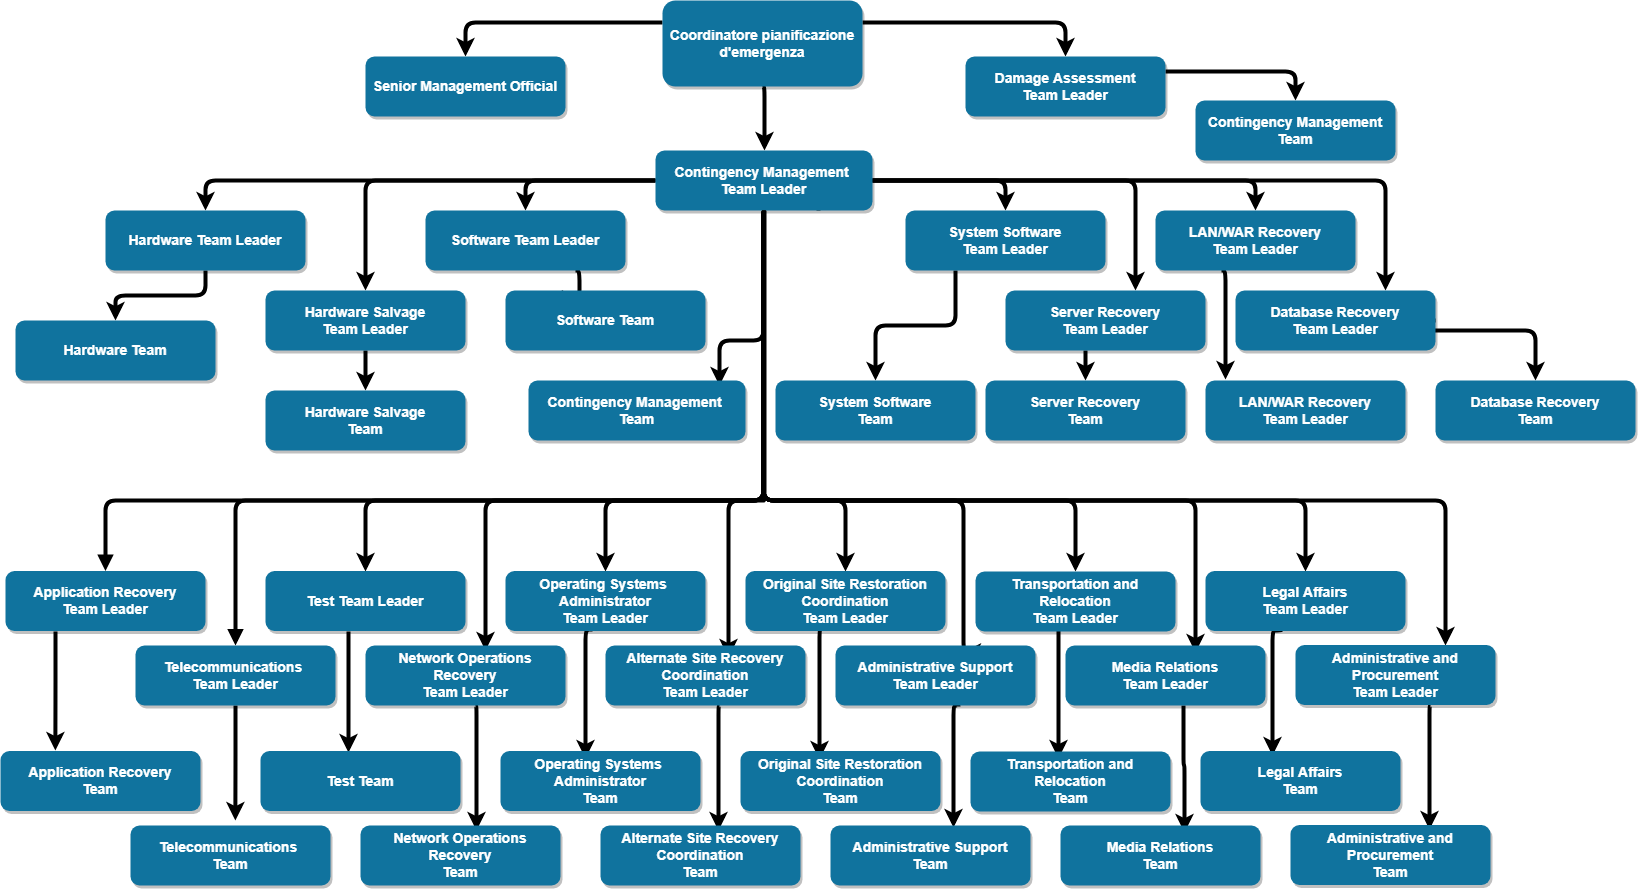
\includegraphics[scale=0.3]{./img/callTree.png}
		\caption{Call tree per la procedura di notifica}
	\end{figure}
	\newpage
	\subsubsection{Struttura della notifica}
	
	È importante specificare il contenuto di una notifica per fare in modo che il personale di recupero conosca il template e trovi velocemente i dettagli su danni e tipologia di disastro. La notifica deve comprendere le seguenti informazioni:
	\begin{itemize}
		\item La natura dell'emergenza che si è verificata o che è imminente;
		\item Se ci sono casi di decesso o lesioni gravi a personale e clienti dell'istituto;
		\item Una stima dei danni noti;
		\item Dettagli di risposta e di recupero;
		\item Istruzioni per preparare il trasferimento verso un sito alternativo per un periodo di tempo stimato;
		\item Istruzioni per completare la fase di notifica utilizzando il call tree.
	\end{itemize}
	Una volta che il CPC ha deciso quale strategia di recupero utilizzare in base alla valutazione sul danno del Damage Assessment Team, sarà sua responsabilità notificare il Contingency Management Team Leader affinché quest'ultimo notifichi, tramite la struttura di notifica appena descritta, i team di recupero più appropriati, in base alla tipologia di danno occorso.
	
	\subsubsection{Ordine di notifica}
	
	La procedura di notifica segue il seguente ordine:
	\begin{enumerate}
		\item Il CPC contatta il Damage Assessment Team Leader in seguito ad un disastro;
		\item Il Damage Assessment Team esegue la valutazione sul danno;
		\item Il Damage Assessment Team Leader contatta il CPC in merito ai risultati della valutazione sul danno;
		\item Se il CPC decide che è opportuno attivare il piano, deve notificare il Contingency Management Team Leader in modo che quest'ultimo notifichi tutti i leader dei team inclusi della procedura di recupero e informi loro riguardo i dettagli dell'evento e se è necessario un trasferimento;
		\item Una volta che i leader dei team di recupero ricevono la notifica da parte del Contingency Management Team Leader, hanno la responsabilità di notificare il proprio team di recupero. I membri del team devono essere informati su tutte le informazioni applicabili e preparati a rispondere e a trasferirsi se necessario;
		\item Il CPC ha il compito di contattare il deposito fuori sede che un evento d'emergenza è stato dichiarato e che è necessario spedire tutti i materiali necessari al sito alternativo. I materiali sono determinati dalla valutazione sul danno;
		\item Il CPC ha il compito di contattare il sito alternativo che un evento d'emergenza è stato dichiarato e di preparare la struttura per l'arrivo del personale dell'istituto;
		\item Il CPC ha il compito di contattare tutto il rimanente personale sullo stato generale dell'incidente. Questo tramite le procedure di notifica descritte in sezione §\ref{procedure}.
	\end{enumerate}
	
	\newpage
	
	\section{Stabilimento di contingency}
	
	In questa sezione vengono presentati gli stabilimenti di contingenza dell'istituto. Gli stabilimenti sono da considerare per quei tipi di disastri con effetti a lungo termine che, anche se rari, sono sempre possibili. Il piano include procedure per ripristinare ed eseguire le operazioni del sistema su un sito alternativo per un periodo di tempo esteso. L'istituto presenta tre tipologie di siti alternativi, di cui due interni, ovvero di proprietà dell'istituto, e uno esterno, di proprietà di un azienda che affitta stabilimenti d'emergenza. I tre siti sono categorizzati in base alla loro prontezza operativa. Sono descritti a partire dal più economico al più dispendioso:
	\begin{itemize}
		\item \textbf{Cold site}: sito con spazio e infrastruttura adeguata per supportare il sistema IT. Il sito non contiene apparecchiatura IT e apparecchiatura d'ufficio, come telefoni o stampanti. Nel caso di attivazione del cold site, sarà responsabilità dell'istituto installare l'apparecchiatura necessaria e le telecomunicazioni;
		\item \textbf{Warm site}: è un sito parzialmente fornito di apparecchiatura IT che contiene parte di hardware, software, telecomunicazioni e alimentatori per il corretto funzionamento del sistema IT in caso d'emergenza. È mantenuto in uno stato operativo pronto a ricevere lo spostamento del personale e delle apparecchiature dell'istituto. Nei casi più gravi potrebbe essere necessario preparare il sito ad ospitare personale di recupero e il sistema IT;
		\item \textbf{Hot site}: è uno spazio propriamente dimensionato per supportare i requisiti del sistema IT che contiene hardware, software, infrastruttura e personale necessari per il recupero del sistema. Il sito è disponibile 24 ore su 24 e 7 giorni la settimana. All'interno è già presente il personale che si occupa di preparare il sito per ospitare il sistema in caso d'emergenza. Alcuni server dell'hot site vengono utilizzati per bilanciare il traffico delle applicazioni dei server primari sul sito principale.
	\end{itemize}
	I siti sono stati valutati dall'istituto in modo che la sicurezza, la gestione, l'operatività e i controlli tecnici siano compatibili con il sito principale.

	
	\subsection{Interni} \label{interni}
	
	Sono gli stabilimenti posseduti e gestiti dall'istituto.
	
	\subsubsection{Cold Standby} \label{cold}
	
	Il cold site è il sito più economico e semplice dell'organizzazione e si trova a Piacenza, Italia. Il sito contiene le risorse minime per ospitare il sistema IT in caso di emergenza. Il sito viene utilizzato per il recupero delle risorse IT di bassa priorità. Se uno dei sistemi in questa lista dovesse smettere di funzionare per un tempo superiore a quello concordato nello SLA è necessario attivare il piano di contingenza e iniziare la mobilitazione di personale e apparecchiature di recupero verso il cold site:
	\begin{itemize}
		\item RAP;
		\item Ican;
		\item Protocollo;
		\item Server Exchange;
		\item Server NTP;
		\item Porta applicativa.
	\end{itemize}
	Per il ripristino dei sistemi sopra elencati è necessaria la seguente apparecchiatura IT, raggruppata per sistema:
	\begin{itemize}
		\item \textbf{RAP}: il ripristino del sistema richiede due sistemi SGI Origin 2000, software FailSafe e software Agent di Oracle;
		\item \textbf{Ican}: il ripristino del sistema richiede un'application server con cluster Santer dove viene installata l'applicazione `soluzione regionale' che comprende il middleware ICan;
		\item \textbf{Protocollo}: il ripristino del sistema richiede un server per hostare l'applicativo che gestisce il protocollo aziendale;
		\item \textbf{Server Exchange}: il ripristino del sistema richiede due server, uno per Exchange 2003 e uno per Exchange 2007;
		\item \textbf{Server NTP}: il ripristino del sistema richiede un server per la sincronizzazione del tempo;
		\item \textbf{Porta applicativa}: il ripristino del sistema richiede server, router, firewall e software necessari alla gestione delle connessioni dall'esterno da parte dei medici di medicina generale e di medici di altre AO per la visualizzazione dei referti memorizzati sul repository locale.
	\end{itemize}
	Per il corretto funzionamento dell'hardware importato all'interno del cold site è necessario collegare alla rete del sito principale tutti i componenti dell'infrastruttura del sito alternativo.
	Per il ripristino dei sistemi sopra riportati è necessario mobilitare verso il cold site i seguenti team:
	\begin{itemize}
		\item Transportation and Relocation Team;
		\item Original Site Restoration Coordination Team;
		\item Procurement Team;
		\item Hardware Team;
		\item Server Recovery Team;
		\item Off-site Storage Team;
		\item Systems Software Team;
		\item Software Team;
		\item Test Team;
		\item LAN Recovery Team.
	\end{itemize}
	
	\newpage
	
	\subsubsection{Warm Standby} \label{warm}
	
	Il warm site è un sito più costoso e più fornito di apparecchiatura IT rispetto al cold site e si trova a Roma, Italia. Il sito contiene parte dell'hardware, del software e delle telecomunicazioni utili al ripristino del sistema in caso d'emergenza. Il sito viene utilizzato per il recupero delle risorse IT con media priorità di ripristino. Se uno dei sistemi in questa lista dovesse smettere di funzionare per un tempo superiore a quello concordato nello SLA è necessario attivare il piano di contingenza e iniziare la mobilitazione di personale e apparecchiature di recupero mancante verso il warm site:
	\begin{itemize}
		\item Armonia;
		\item Aliseo;
		\item Server WINS;
		\item Backup;
		\item Accesso remoto;
		\item Repository.
	\end{itemize}
	Si è deciso di predisporre il sito con le apparecchiature IT e i dispositivi di rete utili al recupero delle applicazioni con media priorità di ripristino più pesanti. Per le restanti applicazioni esiste un contratto con \vendor{} per la mobilitazione dell'apparecchiatura necessaria al momento dell'attivazione del piano.
	Nel sito sono già presenti le seguenti apparecchiature IT, raggruppate per sistema:
	\begin{itemize}
		\item \textbf{Aliseo}: due sistemi SGI Altix350, ciascuno con 2 processori Mips R16k a 800MHz e 16 GB di memoria, con doppio alimentatore ridondato e uno storage della famiglia InfiniteStorage modello TP9300 con 14 dischi da 146GB SCSI, per una capacità totale di 2TB raw, ed interconnessione in FiberChannel a 2Gbit per una bandwidth complessiva fino a 800Mbytes/sec. Su questi server è installato il DB Oracle versioni 9i e 10g Enterprise (4 processori) in modalità RACK su cui sono memorizzati i dati dell'applicativo Aliseo per la gestione del personale;
		\item \textbf{Repository}:  due server (HP DL380 con storage condiviso HP MSA 1000 con 8 HD da 72GB) con SO Linux (RedHat Enterprise v.3 upd. 6), identici dal punto di vista hardware e software, in cui però i servizi realmente attivi sono suddivisi tra le due macchine. Sui server è installata la `soluzione generale' che comprende il software di base per il repository;
		\item \textbf{Backup}: HP Tape Library per un utilizzo con il server di backup e un server per hostare l'applicazione che permette il backup.
	\end{itemize}
	Per il ripristino dei sistemi sopra elencati è necessaria la seguente apparecchiatura IT aggiuntiva, raggruppata per sistema:
	\begin{itemize}
		\item \textbf{Armonia}: per il ripristino del sistema è necessario un server che ospiti l'applicativo client/server;
		\item \textbf{Server WINS}: per il ripristino del sistema è necessario un server Microsoft Windows 2003;
		\item \textbf{Accesso remoto}: per il ripristino del sistema è necessario un server che ospiti l'applicativo che gestisce l'accesso remoto.
	\end{itemize}
	Per il corretto funzionamento dell'hardware importato all'interno del warm site è necessario collegare alla rete del sito principale tutti i componenti dell'infrastruttura del sito alternativo.
	Per il ripristino dei sistemi sopra riportati è necessario mobilitare verso il warm site i seguenti team:
	\begin{itemize}
		\item Transportation and Relocation Team;
		\item Original Site Restoration Coordination Team;
		\item Procurement Team;
		\item Hardware Team;
		\item Server Recovery Team;
		\item Off-site Storage Team;
		\item Systems Software Team;
		\item Software Team;
		\item Test Team;
		\item LAN Recovery Team.
	\end{itemize}
	
	\subsection{Esterno} \label{esterno}
	
	È uno stabilimento esterno all'azienda, gestito da \hotVendor.
	
	\subsubsection{Hot standby} \label{hot}
	
	È lo stabilimento di proprietà dell'azienda \hotVendor. È stato firmato un contratto a lungo termine con tale azienda che si occupa della gestione e del mantenimento del sito. Per la stipulazione del contratto sono stati negoziati:
	\begin{itemize}
		\item Tempi di testing dello stabilimento;
		\item Requisiti hardware e software;
		\item Requisiti di telecomunicazioni;
		\item Requisiti sui servizi supportati;
		\item Numero di giorni che l'istituto può occupare il sito in caso d'emergenza.
	\end{itemize}
	L'hot site è il sito più costoso e fornito di apparecchiatura IT dell'istituto e si trova a Berlino, Germania. Il sito contiene tutto l'hardware, il software e le telecomunicazioni utili al ripristino del sistema in caso di emergenza. Il sito viene utilizzato per il recupero delle risorse IT con alta priorità di ripristino, ovvero per quelle risorse la cui interruzione comporterebbe gravi impatti e perdite per l'istituto. Se uno dei sistemi in questa lista dovesse smettere di funzionare per un tempo superiore a quello concordato nello SLA è necessario attivare il piano di contingenza e iniziare la mobilitazione di personale verso l'hot site:
	\begin{itemize}
		\item Gestione pagamento ticket;
		\item Archivio clinico;
		\item Argos;
		\item Emonet;
		\item Aurora Web;
		\item GST\_FAT;
		\item PACS;
		\item ORMAWIN2000;
		\item PowerLab;
		\item Enco;
		\item Router Internet;
		\item NETASQ F1000;
		\item Server DNS;
		\item Server DHCP;
		\item Oracle.
	\end{itemize}
	Si è deciso di predisporre il sito con le apparecchiature IT utili al recupero delle applicazioni con alta priorità di ripristino. Per quanto riguarda l'infrastruttura di rete, si è deciso di replicarla nell'hot site. Nel sito sono presenti le seguenti apparecchiature IT, raggruppate per sistema:
	\begin{itemize}
		\item \textbf{Gestione pagamento ticket}: server che ospita l'applicazione che gestisce il pagamento dei ticket da parte degli utenti dell'istituto;
		\item \textbf{Archivio clinico}: server che ospita l'applicazione per la gestione dell'archiviazione delle cartelle cliniche cartacee;
		\item \textbf{Argos}: server che ospita il sistema Teseo per l'elaborazione dei CET Regionali;
		\item \textbf{Emonet}: server che ospita l'applicativo client/server Emonet, richiesto da Regione Lombardia per la gestione delle sacche di plasma;
		\item \textbf{PACS}: apparecchiature server e storage per il funzionamento del sistema RIS/PACS fornito dall'AFGA;
		\item \textbf{ORMAWIN2000}: server che ospita l'applicazione ORMAWIN2000 utilizzata per la gestione dei verbali operatori e delle endoprotesi;
		\item \textbf{Aurora Web, GST\_FAT, PowerLab, Enco}: due sistemi SGI Altix350, ciascuno con 2 processori Mips R16k a 800MHz e 16 GB di memoria, con doppio alimentatore ridondato e uno storage della famiglia InfiniteStorage modello TP9300 con 14 dischi da 146GB SCSI, per una capacità totale di 2TB raw, ed interconnessione in FiberChannel a 2Gbit per una bandwidth complessiva fino a 800Mbytes/sec. Su questi server è installato il DB Oracle versioni 9i e 10g Enterprise (4 processori) in modalità RACK su cui sono memorizzati i dati dei seguenti applicativi: Aurora Web (PS, ADT, CUP), GST (Casse), Powerlab (Lab. Analisi), Enco (amministrazione);
		\item \textbf{Router Internet}: è il router che consente l'accesso ad Internet nell'hot site;
		\item \textbf{NETASQ F1000}: è il firewal dell'hot site;
		\item \textbf{Server DHCP/DNS}: Server Microsoft Windows 2003 con servizi DHCP e DNS;
		\item \textbf{Oracle}: server che ospita il database Oracle dell'hot site.
	\end{itemize}
	Per il ripristino dei sistemi sopra riportati è necessario mobilitare verso l'hot site i seguenti team:
	\begin{itemize}
		\item Transportation and Relocation Team;
		\item Original Site Restoration Coordination Team;
		\item Media Relations Team;
		\item Legal Affairs Team;
		\item Off-site Storage Team;
		\item Software Team;
		\item Test Team;
		\item LAN Recovery Team;
		\item Procurement Team;
		\item Hardware Team;
		\item Server Recovery Team;
		\item Systems Software Team.
	\end{itemize}
	\newpage
	\subsection{Norme sul trasporto dell'apparecchiatura} \label{trasporto}
	
	Nel caso in cui debba essere attivato un cold site e/o un warm site, è necessario che l'apparecchiatura richiesta per il ripristino del sistema IT venga trasportata presso il sito. L'istituto ha stipulato un contratto con l'azienda \vendor{} per il provvigionamento dell'apparecchiatura. Nello SLA che si è stipulato con l'azienda sono stati presi in considerazione i seguenti fattori:
	\begin{itemize}
		\item Hardware, software e apparecchiatura di rete e di telecomunicazioni necessaria per i siti esterni;
		\item La velocità con la quale il venditore deve spedire i componenti necessari dopo essere stato notificato;
		\item La priorità di spedizione delle componenti: se le componenti sono altamente prioritarie, l'azienda si deve impegnare a bloccare le normali vendite per supportare l'istituto in situazione d'emergenza.
	\end{itemize}
	
	\newpage
	
	\section{Procedure operative}
	Questa sezione fornisce le procedure per il ripristino del sistema nel sito alternativo, mentre le attività dirette a riparare i danni al sistema e alle funzionalità originali sono descritte in sezione §\ref{ran}.
	Le operazioni di ripristino iniziano dopo che:
	\begin{itemize}
		\item Il piano di contingenza è stato attivato;
		\item La valutazione sul rischio è stata completata;
		\item Il personale di recupero designato è stato notificato;
		\item I team appropriati sono stati mobilizzati.
	\end{itemize}
	Le attività della fase di ripristino si focalizzano sulle misure di contingenza per eseguire capacità di elaborazione IT temporanee, riparare i danni al sistema originale e ripristinare le capacità operative nella sede principale dell'istituto, o in una nuova sede se ritenuto opportuno.
	I team con responsabilità di recupero devono capire ed essere in grado di applicare le procedure di ripristino illustrate in questa sezione, anche nel caso in cui una copia del piano non fosse disponibile al momento del disastro.
	La sequenza di attività descritta in ogni procedura riflette il tempo di interruzione consentito del sistema per evitare impatti significativi sui sistemi correlati e sulla loro applicazione. Le procedure sono scritte in un formato sequenziale e graduale, in modo che i componenti del sistema possano essere ripristinati in modo logico. Per prevenire difficoltà o confusione durante un'emergenza, nessuno step è dato per assunto o è stato omesso.
	
	\subsection{Cold Standby} \label{procCold}
	
	Questa sezione descrive le procedure per il recupero delle risorse del sistema con bassa priorità di ripristino. Il recupero di queste risorse avviene nel cold site descritto in sezione §\ref{cold} e situato a Piacenza, Italia. Le procedure sono divise per team. Per mantenere un'operatività efficiente, ogni procedura deve essere eseguita nella sequenza in cui viene presentata. Le procedure sono scritte in ordine di priorità di recupero, dal sistema più prioritario al sistema meno prioritario.
	
	\subsubsection{Procedure}
	
	\myparagraph{RAP}\\
	\\L'obiettivo delle procedura è il recupero del sistema \textbf{RAP}:
	\begin{enumerate}
		\procTeam{RAP}
		\hardTeam{RAP}
		\offTeam{RAP}
		\serverTeam{RAP}
		\systTeam{RAP}
		\softTeam{RAP}
		\testTeam{RAP}
		\newpage
		\lanTeam{RAP}
	\end{enumerate}
	
	\myparagraph{Porta applicativa}\\
	\\L'obiettivo delle procedura è il recupero del sistema \textbf{Porta applicativa}:
	\begin{enumerate}
		\procTeam{Porta applicativa}
		\hardTeam{Porta applicativa}
		\offTeam{Porta applicativa}
		\serverTeam{Porta applicativa}
		\systTeam{Porta applicativa}
		\softTeam{Porta applicativa}
		\testTeam{Porta applicativa}
		\lanTeam{Porta applicativa}
	\end{enumerate}
	
	\myparagraph{Server Exchange}\\
	\\L'obiettivo delle procedura è il recupero del sistema \textbf{Exchange}:
	\begin{enumerate}
		\procTeam{Exchange}
		\hardTeam{Exchange}
		\offTeam{Exchange}
		\serverTeam{Exchange}
		\systTeam{Exchange}
		\softTeam{Exchange}
		\testTeam{Exchange}
		\lanTeam{Exchange}
	\end{enumerate}
	
	\myparagraph{Server NTP}\\
	\\L'obiettivo delle procedura è il recupero del sistema \textbf{NTP}:
	\begin{enumerate}
		\procTeam{NTP}
		\hardTeam{NTP}
		\offTeam{NTP}
		\serverTeam{NTP}
		\systTeam{NTP}
		\softTeam{NTP}
		\testTeam{NTP}
		\lanTeam{NTP}
	\end{enumerate}
	
	\myparagraph{Protocollo}\\
	\\L'obiettivo delle procedura è il recupero del sistema di gestione del \textbf{protocollo aziendale}:
	\begin{enumerate}
		\procTeam{di gestione del protocollo aziendale}
		\hardTeam{di gestione del protocollo aziendale}
		\offTeam{di gestione del protocollo aziendale}
		\serverTeam{di gestione del protocollo aziendale}
		\systTeam{di gestione del protocollo aziendale}
		\softTeam{di gestione del protocollo aziendale}
		\testTeam{di gestione del protocollo aziendale}
		\lanTeam{di gestione del protocollo aziendale}
	\end{enumerate}
	
	\myparagraph{ICan}\\
	\\L'obiettivo delle procedura è il recupero del sistema \textbf{ICan}:
	\begin{enumerate}
		\procTeam{ICan}
		\hardTeam{ICan}
		\offTeam{ICan}
		\serverTeam{ICan}
		\systTeam{ICan}
		\softTeam{ICan}
		\testTeam{ICan}
		\lanTeam{ICan}
	\end{enumerate}
	
	\subsection{Warm Standby} \label{procWarm}
	
	Questa sezione descrive le procedure per il recupero delle risorse del sistema con media priorità di ripristino. Il recupero di queste risorse avviene nel warm site descritto in sezione §\ref{warm} e situato a Roma, Italia. Le procedure sono divise per team. Per mantenere un'operatività efficiente, ogni procedura deve essere eseguita nella sequenza in cui viene presentata. Le procedure sono scritte in ordine di priorità di recupero, dal sistema più prioritario al sistema meno prioritario.
	
	\subsubsection{Procedure}
	
	\myparagraph{Aliseo}\\
	\\Per il sistema Aliseo l'Hardware Team e il Procurement Team non sono necessari in quanto l'apparecchiatura IT per tale sistema è già presente e installata presso il warm site.
	L'obiettivo delle procedura è il recupero del sistema \textbf{Aliseo}:
	\begin{enumerate}
		\offTeam{Aliseo}
		\systTeam{Aliseo}
		\softTeam{Aliseo}
		\testTeam{Aliseo}
		\lanTeam{Aliseo}
	\end{enumerate}
	
	\myparagraph{Repository}\\
	\\Per il sistema Repository l'Hardware Team e il Procurement Team non sono necessari in quanto l'apparecchiatura IT per tale sistema è già presente e installata presso il warm site.
	L'obiettivo delle procedura è il recupero del sistema \textbf{Repository-Santer}:
	\begin{enumerate}
		\offTeam{Repository-Santer}
		\systTeam{Repository-Santer}
		\softTeam{Repository-Santer}
		\testTeam{Repository-Santer}
		\lanTeam{Repository-Santer}
	\end{enumerate}
	
	\myparagraph{Backup}\\
	\\Per il sistema di gestione dei backup l'Hardware Team e il Procurement Team non sono necessari in quanto l'apparecchiatura IT per tale sistema è già presente e installata presso il warm site.
	L'obiettivo delle procedura è il recupero del sistema di gestione dei \textbf{backup}:
	\begin{enumerate}
		\offTeam{di gestione dei backup}
		\systTeam{di gestione dei backup}
		\softTeam{di gestione dei backup}
		\testTeam{di gestione dei backup}
		\lanTeam{di gestione dei backup}
	\end{enumerate}
	
	\myparagraph{Accesso remoto}\\
	\\L'obiettivo delle procedura è il recupero del sistema di gestione dell'\textbf{accesso remoto}:
	\begin{enumerate}
		\procTeam{di gestione dell'accesso remoto}
		\hardTeam{di gestione dell'accesso remoto}
		\offTeam{di gestione dell'accesso remoto}
		\systTeam{di gestione dell'accesso remoto}
		\softTeam{di gestione dell'accesso remoto}
		\testTeam{di gestione dell'accesso remoto}
		\lanTeam{di gestione dell'accesso remoto}
	\end{enumerate}
	
	\myparagraph{Server WINS}\\
	\\L'obiettivo delle procedura è il recupero del sistema \textbf{WINS}:
	\begin{enumerate}
		\procTeam{WINS}
		\hardTeam{WINS}
		\offTeam{WINS}
		\systTeam{WINS}
		\softTeam{WINS}
		\testTeam{WINS}
		\lanTeam{WINS}
	\end{enumerate}
	
	\myparagraph{Armonia}\\
	\\L'obiettivo delle procedura è il recupero del sistema \textbf{Armonia}:
	\begin{enumerate}
		\procTeam{Armonia}
		\hardTeam{Armonia}
		\offTeam{Armonia}
		\systTeam{Armonia}
		\softTeam{Armonia}
		\testTeam{Armonia}
		\lanTeam{Armonia}
	\end{enumerate}
	
	\subsection{Hot Standby} \label{procHot}
	
	Questa sezione descrive le procedure per il recupero delle risorse del sistema con alta priorità di ripristino. Il recupero di queste risorse avviene nell'hot site descritto in sezione §\ref{hot} e situato a Berlino, Germania. Le procedure sono divise per team. Per mantenere un'operatività efficiente, ogni procedura deve essere eseguita nella sequenza in cui viene presentata. Le procedure sono scritte in ordine di priorità di recupero, dal sistema più prioritario al sistema meno prioritario. Si fa notare che non sono presenti le procedure di ripristino dei seguenti team:
	\begin{itemize}
		\item LAN Recovery Team: nell'hot site tutte le apparecchiature sono collegate alla rete e pronte;
		\item Procurement Team: nell'hot site sono già presenti tutte le apparecchiature per il ripristino delle risorse con alta priorità di ripristino;
		\item Hardware Team: l'hardware per il recupero dei sistemi è già corretto e funzionante presso l'hot site;
		\item Server Recovery Team: i server sono già configurati presso l'hot site;
		\item Systems Software Team: i sistemi operativi, i sistemi IT e le applicazioni sono già installate sui server dell'hot site.
	\end{itemize}
	
	\subsubsection{Procedure di ripristino}
	
	\myparagraph{Emonet}\\
	\\L'obiettivo delle procedure è il recupero del sistema \textbf{Emonet}:
	\begin{enumerate}
		\offTeam{Emonet}
		\softTeam{Emonet}
		\testTeam{Emonet}
	\end{enumerate}
	
	\myparagraph{Aurora Web, GST\_FAT, PowerLab, Enco}\\
	\\L'obiettivo delle procedure è il recupero del sistema \textbf{Aurora Web, GST\_FAT, PowerLab, Enco}:
	\begin{enumerate}
		\offTeam{Aurora Web, GST\_FAT, PowerLab, Enco}
		\softTeam{Aurora Web, GST\_FAT, PowerLab, Enco}
		\testTeam{Aurora Web, GST\_FAT, PowerLab, Enco}
	\end{enumerate}
	
	\myparagraph{Argos}\\
	\\L'obiettivo delle procedure è il recupero del sistema \textbf{Argos}:
	\begin{enumerate}
		\offTeam{Argos}
		\softTeam{Argos}
		\testTeam{Argos}
	\end{enumerate}
	
	\myparagraph{PACS}\\
	\\L'obiettivo delle procedure è il recupero del sistema \textbf{PACS}:
	\begin{enumerate}
		\offTeam{PACS}
		\softTeam{PACS}
		\testTeam{PACS}
	\end{enumerate}
	
	\myparagraph{ORMAWIN2000}\\
	\\L'obiettivo delle procedure è il recupero del sistema \textbf{ORMAWIN2000}:
	\begin{enumerate}
		\offTeam{ORMAWIN2000}
		\softTeam{ORMAWIN2000}
		\testTeam{ORMAWIN2000}
	\end{enumerate}
	
	\myparagraph{Gestione pagamento ticket}\\
	\\L'obiettivo delle procedure è il recupero del sistema di \textbf{gestione del pagamento dei ticket}:
	\begin{enumerate}
		\offTeam{di gestione del pagamento dei ticket}
		\softTeam{di gestione del pagamento dei ticket}
		\testTeam{di gestione del pagamento dei ticket}
	\end{enumerate}
	
	\myparagraph{Oracle}\\
	\\L'obiettivo delle procedure è il recupero del sistema \textbf{Oracle}:
	\begin{enumerate}
		\offTeam{Oracle}
		\softTeam{Oracle}
		\testTeam{Oracle}
	\end{enumerate}
	
	\myparagraph{Archivio clinico}\\
	\\L'obiettivo delle procedure è il recupero del sistema di gestione dell'\textbf{archivio clinico}:
	\begin{enumerate}
		\offTeam{di gestione dell'archivio clinico}
		\softTeam{di gestione dell'archivio clinico}
		\testTeam{di gestione dell'archivio clinico}
	\end{enumerate}

	
	\subsubsection{Procedure amministrative}
	
	In questa sezione sono trattate le procedure amministrative che devono essere eseguite quando viene attivato l'hot site. Le procedure sono ordinate per team:
	\begin{enumerate}
		\item \textbf{Transportation and Relocation Team}:
			\begin{itemize}
				\item Il team deve coordinare il trasporto dei dipendenti dell'istituto verso l'hot site;
				\item Il team deve coordinare il trasporto dei pazienti dell'istituto verso l'hot site.
			\end{itemize}
		\item \textbf{Media Relations Team}:
			\begin{itemize}
				\item Il team deve occuparsi di contattare i giornali e notiziari locali;
				\item Il team deve accordarsi con i titolari dei giornali locali per evitare rischi d'immagine all'istituto;
				\item Il team deve accordarsi con i titolari dei notiziari locali per evitare rischi d'immagine all'istituto.
			\end{itemize}
		\item \textbf{Legal Affairs Team}:
			\begin{itemize}
				\item Il team deve mettersi in contatto con il legale dell'istituto;
				\item Il team deve prepararsi a possibili accuse contro l'istituto.
			\end{itemize}
	\end{enumerate}
	
	\newpage
	
	\section{Sicurezza}
		\subsection{Dati} \label{dati}
			In questa sezione viene trattata la sicurezza dei dati.
			\subsubsection{Security policy}
			Lo scopo della security policy è informare tutto il personale della necessità di migliorare e mantenere la sicurezza del sistema informativo. Lo scopo di quest'ultima è assicurare un appropriato livello di riservatezza, integrità e disponibilità.\\
			Mantenere l'integrità e la sicurezza dei dati di sistema e del software è un fattore chiave nella pianificazione d'emergenza. L'integrità implica il mantenimento sicuro e accurato dei dati sui dispositivi di archiviazione del sistema. Esistono diversi metodi disponibili per mantenere l'integrità dei dati memorizzati. \\
			La sicurezza implica la protezione dei dati sia in sede che fuori sede da accessi o utilizzi non autorizzati. La crittografia è un metodo comune per la protezione dei dati di sistema memorizzati. Essa è più efficace se applicata sia al dispositivo di archiviazione dati primario che ai supporti di backup che si trovano nel magazzino di \backupVendor. Se si utilizza la crittografia per la memorizzazione dei dati fuori sede, è importante che i lettori multimediali (ad esempio unità nastro, lettori CD o DVD) siano disponibili nel sito alternativo, per leggere correttamente i dati crittografati durante il ripristino.
			È necessario stabilire un solido processo di gestione delle chiavi in modo che i dati crittografati siano disponibili, se necessario. Il metodo utilizzato per stabilire e mantenere le chiavi deve essere gestito, idealmente, in una posizione centrale all'interno dell'organizzazione. Queste chiavi devono essere archiviate separatamente dai dati di backup primari crittografati, ma devono essere accessibili.
		
			\subsubsection{Autenticazione}
			L'autenticazione ai componenti del sistema informativo, in particolare alle postazioni dei dipendenti, avviene solamente utilizzando le credenziali fornite dall'istituto al personale. Ogni individuo è responsabile della protezione della propria password e di altri meccanismi di autenticazione (come nomi utente, PIN); inoltre deve assicurarsi che non vengano né divulgati né utilizzati da nessun altro, in nessuna circostanza. Tutto il personale è responsabile per qualsiasi attività svolta con le loro credenziali.
			Valgono le seguenti regole:
			\begin{itemize}
				\item Le password devono avere una lunghezza minima di 8 caratteri e devono essere costituite da una combinazione di caratteri alfanumerici;
				\item Le modifiche alle password sono richieste ogni 180 giorni al minimo o immediatamente se compromesse. Il sistema fa scadere automaticamente le password ad intervalli regolari e richiede all'utente di reimpostare la password;
				\item Le password dovrebbero essere memorizzate e mai scritte;
				\item Le password non devono essere archiviate in formato elettronico nei file del computer o su dispositivi portatili, a meno che non siano fortemente crittografate. Questa metodologia non è sicura in caso di malfunzionamento del dispositivo su cui la password è salvata, in quanto potrebbe non essere recuperabile;
				\item Le password non devono essere inserite nei messaggi di posta elettronica o in altre forme di comunicazione elettronica senza l'uso della crittografia;
				\item Non utilizzare la stessa password di altri account;
				\item La funzionalità di ``blocco" della password è abilitata su qualsiasi sistema in cui sia disponibile e ragionevole da implementare. Gli utenti saranno esclusi dai sistemi dopo fallito 5 tentativi in 1 minuto per accedere alla postazione. Questo richiederà l'intervento dell'help desk per riottenere l'accesso.
			\end{itemize}
		
		\subsubsection{Controllo e accesso della rete}
		Di seguito sono riportate le linee guida per la sicurezza della rete aziendale:
		\begin{itemize}
			\item Chiunque usi l'ambiente di calcolo dell'istituto deve essere adeguatamente autorizzato;
			\item Gli utenti non devono:
			\begin{itemize}
				\item Compiere atti che abbiano un impatto negativo sul funzionamento di computer, periferiche, reti o che impediscano a qualcun altro di svolgere il proprio lavoro; 
				\item Tentare di aggirare i regimi di protezione per l'accesso a dati o sistemi; 
				\item Ottenere o concedere l'accesso non autorizzato a computer, dispositivi, software o dati. 
			\end{itemize}
			\item Gli utenti possono essere ritenuti legalmente e finanziariamente responsabili delle azioni risultanti dall'uso non autorizzato di account di rete e di sistema dell'istituto;
			\item L'azienda ha installato vari dispositivi di sicurezza di rete, tra cui firewall per garantire la sicurezza e la protezione delle informazioni dell'istituto. Qualsiasi tentativo di disabilitare, sconfiggere o aggirare qualsiasi struttura di sicurezza è considerato un'attività inappropriata ed è una violazione di questa politica di rete;
			\item L'espansione o la manipolazione dell'hardware di rete e/o del software, ad eccezione di individui designati all'interno della divisione IT, senza previa approvazione da parte della divisione IT, è severamente vietata;
			\item Prima di collegare qualsiasi server alla rete dell'istituto, deve essere ottenuta l'approvazione per iscritto dalla divisione IT dell'azienda stessa;
			\item È severamente vietato l'accesso alla rete di altri eventuali dispositivi diversi da quelli forniti o approvati dalla divisione IT;
			\item L'assegnazione statica di indirizzi IP non approvati e non ottenuti dalla divisione IT non è consentita;
			\item Solo il personale della divisione IT o gli agenti autorizzati possono spostare le apparecchiature di rete e di comunicazione di proprietà dell'istituto;
			\item I proprietari dei dati memorizzati su sistemi accessibili alla rete sono responsabili della gestione e della determinazione dell'appropriatezza delle informazioni memorizzate su questi sistemi. Ciò include sia aree di archiviazione private che aree di cartelle ``condivise";
			\item È vietato l'accesso e l'installazione di server DHCP o DNS non autorizzati.
		\end{itemize}
		
		\subsubsection{Sicurezza dei backup}
		Un efficace processo di backup dei dati è cruciale per la strategia di recupero globale del CPC. I backup dei dati devono essere disponibili, integri e riservati in quanto contengono dati sensibili.
		I backup possono essere mantenuti internamente all'azienda oppure possono essere memorizzati presso un fornitore esterno. Nell'ultimo caso dovranno essere concordate e successivamente mantenute delle policy di sicurezza con il fornitore del servizio di backup \backupVendor. I dati devono essere protetti anche durante il trasporto dal sito primario al sito del fornitore, qualunque sia il mezzo di trasporto.
		I dati vengono resi sicuri effettuando nigthly backup presso un fornitore \backupVendor.
		Nel processo di scelta di un fornitore di servizi che manterrà o accederà regolarmente a dati, informazioni e risorse coperti, il processo di valutazione includerà la capacità del fornitore di servizi di	salvaguardare informazioni riservate. 
		I contratti con i fornitori di servizi possono includere le seguenti disposizioni:
		\begin{itemize}
			\item Riconoscimento esplicito che il contratto consente al partner contrattuale di accedere a informazioni riservate;
			\item Una specifica definizione o descrizione delle informazioni riservate fornite; \item una clausola secondo cui le informazioni riservate saranno conservate con la massima riservatezza e accessibili solo per l'esplicito scopo commerciale del contratto; 
			\item Una garanzia da parte del partner contrattuale che il partner proteggerà le informazioni riservate che riceve secondo standard commercialmente accettabili e non meno rigorosamente di quanto non protegga le proprie informazioni riservate; 
			\item Una disposizione che preveda la restituzione o la distruzione di tutte le informazioni riservate ricevute dal fornitore del contratto al completamento o alla risoluzione del contratto; 
			\item Un accordo sul fatto che qualsiasi violazione delle condizioni di riservatezza del contratto può costituire una violazione materiale del contratto e autorizza l'istituto a risolvere il contratto senza penalità;
			\item Una disposizione che garantisca che i requisiti di riservatezza del contratto sopravvivranno a qualsiasi accordo di risoluzione.
		\end{itemize}
		
		\subsubsection{Software per la sicurezza}
		\begin{itemize}
			\item Tutti i computer dell'azienda hanno installato il software antivirus standard scelto dal dipartimento IT dell'istituto. Il software e le definizioni dei virus devono essere aggiornati. È compito degli amministratori della rete verificare che il software antivirus sia attivo, che funzioni correttamente e che i computer non contengano virus. I computer infettati da virus possono essere rimossi dalla rete finché non vengono dichiarati come esenti da virus. Qualsiasi attività con l'intenzione di creare e/o distribuire programmi dannosi all'interno della rete è proibita;
			\item Il software di monitoraggio esamina periodicamente l'attività sui sistemi, cercando gli indicatori di compromesso configurati dall'amministrazione e talvolta attivando le notifiche quando vengono raggiunte determinate soglie;
			\item Le utilità di registrazione (Logging Utilities) forniscono evidenza dell'attività sul sistema che può essere utilizzata per controllare l'accesso e identificare gli incidenti.
			\item La crittografia a livello di file o di intero disco impedisce l'accesso non autorizzato ai dati codificando file, cartelle o interi sistemi operativi, in modo tale che solo le persone autorizzate possano ottenere l'accesso.
		\end{itemize}
		
		
		\subsubsection{Licenze software}
		\begin{itemize}
			\item Tutti i software utilizzati dall'istituto sono protetti da copyright e il personale può usarli solo in base ai termini della licenza ottenuta;
			\item La duplicazione di software con l'intento di ridistribuirlo senza autorizzazione è proibita;
			\item Tutti gli utenti sono legalmente responsabili nei confronti dell'emittente della licenza o del titolare del copyright;
			\item È severamente proibito l'inserimento di software ottenuti illegalmente su computer dell'azienda.
		\end{itemize}
	
		\subsubsection{Distruzione e smaltimento di informazioni e dispositivi}
		Le informazioni riservate devono essere smaltite in modo tale da garantire che non possano essere recuperate da persone non autorizzate. Di seguito vengono riportati i punti da seguire:
		\begin{itemize}
			\item I documenti cartacei devono essere triturati;
			\item Quando si effettua la donazione, la vendita, il trasferimento, l'eccedenza o lo smaltimento di computer o supporti rimovibili, è necessario prestare attenzione per garantire che i dati riservati siano resi illeggibili. Qualsiasi informazione riservata archiviata deve essere completamente distrutta. In generale, non è sufficiente ``cancellare" l'informazione, poiché potrebbe rimanere sul supporto. I dati devono essere correttamente rimossi dall'unità da un software o l'unità può essere fisicamente distrutta.
		\end{itemize}	
	
		
		\subsection{Infrastruttura} \label{infrastruttura}
		Per quanto riguarda l'infrastruttura del sito primario e dei siti di contingency, sono presenti alcuni sistemi che garantiscono sicurezza sia durante il normale funzionamento, sia in situazioni di emergenza.
		I sistemi installati negli stabilimenti sono:
		\begin{itemize}
			\item Condizionamento;
			\item Gruppi di continuità;
			\item Controllo accessi;
			\item Videosorveglianza;
			\item Antincendio.
		\end{itemize}
		Di seguito ogni sistema verrà descritto.
			\subsubsection{Condizionamento}
			All'interno del CED è presente un sistema di condizionamento per mantenere una temperatura il più possibile vicino ai \SI{21}{\celsius} e comunque sempre all'interno dell'intervallo \SI{18}{\celsius} - \SI{24}{\celsius}. Inoltre, il livello di umidità all'interno del CED deve rimanere il più possibile all'interno dei valori 40\% - 60\%. 
			Ogni attività all'interno del CED deve essere focalizzata sulla conservazione delle temperature e dei livelli di umidità ottimali. Le apparecchiature di condizionamento non devono mai essere ostruite, e ogni alterazione o manutenzione delle stesse, deve essere concordata con il responsabile. Il risultato di ogni modifica e manutenzione deve essere documentato.
			
			\subsubsection{Gruppi di continuità}
			Nell'infrastruttura di rete sono presenti dei gruppi di continuità (UPS) per mantenere elettricità in caso venisse a mancare, in modo tale da non interrompere le normali attività dell'azienda. Ogni componente critico dell'infrastruttura di rete ha un UPS associato. I gruppi di continuità devono essere sempre operativi e funzionanti, per questo motivo periodicamente vengono sottoposti a manutenzione, previo accordo con il responsabile. 
			
			\subsubsection{Controllo accessi}
			L'azienda è dotata di terminali Zucchetti dedicati alla rilevazione presenze e al controllo degli accessi.
			Il controllo degli accessi comprende dei lettori badge per la gestione delle presenze. 
			Questi sistemi sono necessari in quanto all'interno dell'ospedale sono presenti spazi aperti al pubblico, spazi privati e aree accessibili solamente da personale autorizzato. Ogni area richiede un diverso livello di sicurezza e l'accesso è consentito solamente a persone autorizzate tramite badge. Non è possibile accedere alle aree senza il riconoscimento.
			
			\subsubsection{Videosorveglianza}
			L'istituto è dotato anche di un sistema di videosorveglianza per monitorare l'intera struttura. Le telecamere sono installate in modo tale da controllare ogni entrata e uscita alla struttura. I filmati sono visibili in tempo reale da una sala di vigilanza e successivamente vengono memorizzati su un server.
			
			\subsubsection{Antincendio}
			All'interno dell'istituto è presente un sistema antincendio che entra in funzione quando si verifica un incendio. Il sistema è sottoposto a manutenzioni periodiche in quanto deve essere sempre funzionante e attivo. Nel caso si debba disattivarlo è necessaria l'approvazione del responsabile.
			
			
		\subsection{Personale} \label{sicPersonale}
			La pianificazione d'emergenza informatica è specifica per le misure di recupero per i sistemi di supporto generale e le principali applicazioni; tuttavia, tali piani vengono raramente sviluppati o eseguiti da soli. Quando si verifica un incidente che influisce sulle operazioni IT, spesso influisce sul personale dell'organizzazione. Devono essere pianificate adeguate considerazioni per la sicurezza e il benessere del personale, in previsione di un evento dirompente. Le procedure di evacuazione e il riottenere l'accesso alla struttura dovrebbero essere coordinati ed esercitati congiuntamente con le autorità locali. Le organizzazioni dovrebbero anche disporre di metodi e standard per interfacciarsi con le richieste dei media e inviare messaggi reattivi al personale. 
			
			\subsubsection{Sicurezza ed evacuazione del personale}
				La sicurezza e l'evacuazione del personale durante e dopo un'interruzione sono tipicamente affrontati in un piano di emergenza degli occupanti (OEP). Il personale deve essere a conoscenza delle procedure di sicurezza e di uscita e deve allenarsi a svolgere queste procedure durante le normali esercitazioni antincendio. Gli OEP e i piani di emergenza IT possono includere istruzioni per la sicurezza di spazi per uffici, workstation personali e computer portatili per impedire l'accesso alle informazioni e ridurre la probabilità di atti vandalici o furti. I piani possono anche includere promemoria per raccogliere identificazioni, le chiavi delle macchine e altri beni importanti, se la natura dell'incidente e il tempo lo consentono. Inoltre, potrebbe essere necessario che le procedure descrivano il modo in cui riottenere l'accesso. Le istruzioni più appropriate per uscire dalla struttura sono basate sui requisiti specifici del sito e sulle normative locali sui codici antincendio. Una metodologia di ``custode del piano" può essere incorporata nel piano e istituita come una pratica normale. Questa metodologia prevede la designazione e la formazione di una o due persone specifiche di ogni piano per essere responsabile dell'evacuazione di tutto il personale. Questa responsabilità di solito ruota in modo tale che le stesse persone non siano responsabili di sorvegliare le evacuazioni durante tutto l'anno.\\
				\\L'OEP dovrebbe includere anche procedure e metodi di contatto multipli per la raccolta di personale dopo il disastro. È importante che l'alta direzione sappia chi era nell'edificio prima dell'evento e chi è stato tenuto in considerazione (sia in loco che fuori sede) in modo che le autorità civili (vigili del fuoco, polizia, soccorso) e le famiglie possano essere adeguatamente informate della situazione. Dovrebbero essere sviluppate procedure per istruire il personale a incontrarsi in uno specifico sito pianificato in precedenza, lontano dall'edificio. Al personale dovrebbero essere fornite procedure alternative per contattare l'organizzazione e fornire informazioni sulla loro ubicazione nel caso in cui la posizione non sia sicura. Una metodologia di reporting centralizzata ridurrà possibili confusioni e informazioni contrastanti. I metodi di contatto possono essere sviluppati per essere inviati e/o ricevuti per telefono, posta elettronica (e-mail), messaggistica istantanea (IM), riunione in un luogo fisico o da una combinazione di metodi. Questa informazione può essere stampata su su carta, insieme a informazioni di contatto dei colleghi, e rilasciata al personale per essere archiviata con i loro badge di identificazione come una pratica normale.
				
			\subsubsection{Benessere del personale}
				Durante una situazione seria, affrontare il personale e le questioni familiari spesso ha la priorità sulla ripresa degli affari. La pianificazione di tali questioni può comportare la pre-identificazione di alloggi temporanei, aree di lavoro e personale. In alcune situazioni, l'organizzazione potrebbe dover utilizzare personale di organizzazioni associate o stipulare contratti con fornitori o consulenti se i membri del team principale e alternativo non sono disponibili o non sono in grado di adempiere alle responsabilità. I preparativi dovrebbero essere fatti durante lo sviluppo del piano d'emergenza per garantire che i venditori o i consulenti possano ottenere lo stesso accesso dei membri del team in caso di disastro. Una volta che il personale è pronto per tornare al lavoro, devono essere presi accordi affinché possano lavorare in un sito alternativo o a casa se la struttura non è sicura o non è disponibile per l'uso. Questo è uno spazio alternativo oltre al sito alternativo per le operazioni di emergenza IT. Al personale con computer o laptop domestici dovrebbe essere fornita l'istruzione su come accedere alla rete dell'organizzazione da casa. Potrebbe anche essere necessario assistere il personale con l'acquisto di alloggi temporanei.\\
				\\I disastri possono richiedere un pesante impatto psicologico al personale, specialmente se si è verificata una perdita di vite umane o un'estesa distruzione fisica. Le organizzazioni dovrebbero essere preparate a fornire consulenza per il dolore e altro supporto per la salute mentale. Dovrebbe essere fatto ogni sforzo per continuare a pagare il personale secondo le normali operazioni. A causa del dolore e dello stress, la produttività potrebbe anche essere bassa durante il periodo di adattamento.
				
			\subsubsection{Rapporti con le organizzazioni di risposta}
				Una relazione deve essere costruita con i dipartimenti locali di vigili del fuoco e di polizia, al fine di ottenere una comprensione approfondita delle procedure e di instaurare un rapporto di fiducia, in modo che l'organizzazione non incontri per la prima volta i dipartimenti locali di polizia e vigili del fuoco in caso di calamità. I funzionari dei vigili del fuoco e della polizia possono assumere l'autorità sulla struttura, se la situazione lo giustifica. L'organizzazione deve essere consapevole del motivo per cui ciò può accadere e quali Point Of Contact (POC) e documentazione saranno necessari per riottenere l'accesso alla struttura. Le organizzazioni di vigili del fuoco, di polizia e di soccorso sono spesso disposte a collaborare con l'organizzazione per sviluppare procedure sicure e coordinate, e partecipare agli esercizi dell'organizzazione. Sulla base delle esigenze dell'organizzazione, potrebbero anche essere necessarie pianificazioni congiunte ed esercitazioni.
				
			\subsubsection{Pianificazione della continuità}
				Il piano di comunicazione della crisi generalmente affronta i flussi di comunicazione interna con il personale e management, e la comunicazione esterna con il pubblico. Il modo più efficace per fornire informazioni utili e ridurre le voci è comunicare in modo chiaro e frequente. Il piano dovrebbe anche preparare l'organizzazione alla possibilità che durante un disastro significativo l'organizzazione possa essere un punto di inoltro delle comunicazioni tra il personale, le autorità e le famiglie o gli amici interessati.\\
				\\Una delle attività più importanti è la comunicazione all'interno dell'organizzazione. Il personale e il management devono sapere cosa è successo, lo stato della situazione, quali azioni dovrebbero intraprendere e chi è responsabile della situazione. Una persona o gruppo dovrebbe essere responsabile per la comunicazione interna. Questa persona dovrebbe avere accesso alla leadership senior dell'organizzazione. Inoltre, l'organizzazione dovrebbe essere preparata a utilizzare più metodi di comunicazione quali cellulare, e-mail e onde radio. Comunicazioni chiare e frequenti da parte di alti dirigenti a tutto il personale, i POC interconnessi e gli utenti finali sono necessarie dopo un'interruzione per aiutare a calmare l'ansia, e a rispondere a domande di carattere generale.\\
				\\Come la comunicazione interna, l'organizzazione dovrebbe prestare attenzione al messaggio che viene comunicato alle parti esterne. Ancora una volta, un metodo efficace è quello di designare un POC specifico o un team dell'organizzazione per essere responsabile dei comunicati stampa e della comunicazione dei media. Il personale dovrebbe essere addestrato a indirizzare tutte le richieste dei media a un singolo POC o ad un ufficio di informazioni pubbliche senza fare commenti per conto dell'organizzazione. Queste procedure possono anche essere indicate nell'OEP o nella guida dell'ufficio di informazioni pubbliche.
				 
	\newpage
	
	\section{Ritorno alla normalità} \label{ran}
	
	Nella fase di ritorno alla normalità, le attività di ripristino sono terminate e le normali operazioni devono essere ritrasferite nella sede principale dell'istituto. Se la sede originale non è recuperabile, le attività in questa fase devono essere applicate anche per costruire e preparare una nuova sede atta ad ospitare il sistema IT dell'istituto. Una volta che il sito principale, o il nuovo sito, sono pronti per supportare il sistema IT e i suoi processi di routine, il sistema può essere trasferito dal sito alternativo al sito primario. Il sistema d'emergenza deve continuare ad essere operativo fino a quando il sistema primario non è ripristinato. In questa fase vengono specificati i team responsabili per il ripristino del sito principale e del sistema IT. I team devono essere in grado di eseguire le funzioni richieste senza una copia del piano di contingenza, in quanto la documentazione potrebbe non essere disponibile durante una situazione d'emergenza. L'obiettivo della fase di ritorno alla normalità è fornire una trasparente transizione delle operazioni dal sito alternativo al sito principale.
	
	\subsection{Avvio} \label{avvio}
	
	Nel momento in cui le procedure di ripristino sono state completate e il sistema d'emergenza è in uno stato funzionante, l'Alternate Site Recovery Coordination Team deve:
	\begin{itemize}
		\item Fare una valutazione più dettagliata dei danni subiti all'installazione e alle apparecchiature del sito principale;
		\item In base alla valutazione sul danno deve fornire al Contingency Management Team le informazioni necessarie per determinare se il ritorno alla normalità debba orientarsi verso il ritrasferimento o verso la costruzione di un nuovo sito.
	\end{itemize}
	In ogni caso il sistema d'emergenza deve continuare a funzionare durante il recupero del sistema principale. Una volta che il sistema principale è stato recuperato, il piano può essere disattivato. Questa sezione include le procedure per:
	\begin{enumerate}
		\item Ricostruire il sito principale o costruire un nuovo sito;
		\item Mantenere il sistema d'emergenza operativo fino a quando il sistema primario non viene trasferito completamente;
		\item Disattivare il piano di contingenza.
	\end{enumerate}
	Una volta che la ricostruzione è stata avviata, i team necessari per poterla attuare devono essere inviati al sito da ricostruire.
	
	\subsection{Cold Standby} \label{ranCold}
	
	Questa sezione contiene le procedure per ricostruire il sito principale, o costruire un nuovo sito se il principale fosse irrecuperabile, in seguito ad un'interruzione di uno o più servizi con bassa priorità di ripristino. Sono contenute inoltre le procedure per ripristinare il sistema sul sito originale o il nuovo sito, e le procedure per disattivare il piano sul cold site. Le procedure sono divise per team e sono inserite in ordine propedeutico. Le procedure si occupano di ricostruire i seguenti sistemi IT presso il sito principale o un nuovo sito:
	\begin{itemize}
		\item RAP;
		\item Ican;
		\item Protocollo;
		\item Server Exchange;
		\item Server NTP;
		\item Porta applicativa.
	\end{itemize}
	
	\subsubsection{Procedure di ricostruzione}
	
	\myparagraph{RAP}\\
	\ricostruzione{RAP}
	
	\myparagraph{ICan}\\
	\ricostruzione{ICan}
	
	\myparagraph{Protocollo aziendale}\\
	\ricostruzione{di gestione del protocollo aziendale}
	
	\myparagraph{Exchange}\\
	\ricostruzione{Exchange}
	
	\myparagraph{NTP}\\
	\ricostruzione{NTP}
	
	\myparagraph{Porta applicativa}\\
	\ricostruzione{Porta applicativa}
	
	\newpage
	
	\subsubsection{Procedure di trasferimento}
	
	\myparagraph{RAP}\\
	\trasferimento{RAP}
	
	\myparagraph{ICan}\\	
	\trasferimento{ICan}
	
	\myparagraph{Protocollo aziendale}\\
	\trasferimento{di gestione del protocollo aziendale}
	
	\myparagraph{Exchange}\\
	\trasferimento{Exchange}
	
	\myparagraph{NTP}\\
	\trasferimento{NTP}
	
	\myparagraph{Porta applicativa}\\
	\trasferimento{Porta applicativa}
	
	
	\subsubsection{Procedure di disattivazione}
	  	
	  	\myparagraph{RAP}\\
		\disattivazioneColdWarm{RAP}
		
		\myparagraph{ICan}\\		
		\disattivazioneColdWarm{ICan}
		
		\myparagraph{Protocollo aziendale}\\
		\disattivazioneColdWarm{di gestione del protocollo aziendale}
		
		\myparagraph{Exchange}\\
		\disattivazioneColdWarm{Exchange}
		
		\myparagraph{NTP}\\
		\disattivazioneColdWarm{NTP}
		
		\myparagraph{Porta applicativa}\\
		\disattivazioneColdWarm{Porta applicativa}

	
	\subsection{Warm Standby} \label{ranWarm}
	
	Questa sezione contiene le procedure per ricostruire il sito principale, o costruire un nuovo sito se il principale fosse irrecuperabile, in seguito ad un interruzione di uno o più servizi con media priorità di ripristino. Sono contenute inoltre le procedure per ripristinare il sistema sul sito originale o il nuovo sito, e le procedure per disattivare il piano sul warm site. Le procedure sono divise per team e sono inserite in ordine propedeutico. Le procedure si occupano di ricostruire i seguenti sistemi IT presso il sito principale o un nuovo sito:
	\begin{itemize}
		\item Armonia;
		\item Aliseo;
		\item Server WINS;
		\item Backup;
		\item Accesso remoto;
		\item Repository.
	\end{itemize}
	
	\subsubsection{Procedure di ricostruzione}
	
	\myparagraph{Armonia}\\
	\ricostruzione{Armonia}
	
	\myparagraph{Aliseo}\\
	\ricostruzione{Aliseo}
	
	\myparagraph{WINS}\\
	\ricostruzione{WINS}
	
	\myparagraph{Backup}\\
	\ricostruzione{di gestione dei backup}
	
	\myparagraph{Accesso remoto}\\
	\ricostruzione{di gestione dell'accesso remoto}
	
	\myparagraph{Repository-Santer}\\	
	\ricostruzione{Rpository-Santer}

	
	\subsubsection{Procedure di trasferimento}
	
	\myparagraph{Armonia}\\
	\trasferimento{Armonia}
	
	\myparagraph{Aliseo}\\
	\trasferimento{Aliseo}
	
	\myparagraph{WINS}\\
	\trasferimento{WINS}
	
	\myparagraph{Backup}\\
	\trasferimento{di gestione dei backup}
	
	\myparagraph{Accesso remoto}\\
	\trasferimento{di gestione dell'accesso remoto}
	
	\myparagraph{Repository-Santer}\\
	\trasferimento{Repository-Santer}
	
	\newpage
	
	\subsubsection{Procedure di disattivazione}
	
	\myparagraph{Armonia}\\
	\disattivazioneColdWarm{Armonia}
	
	\myparagraph{Aliseo}\\
	\disattivazioneColdWarm{Aliseo}
	
	\myparagraph{WINS}\\
	\disattivazioneColdWarm{WINS}
	
	\myparagraph{Backup}\\
	\disattivazioneColdWarm{di gestione dei backup}
	
	\myparagraph{Accesso remoto}\\
	\disattivazioneColdWarm{di gestione dell'accesso remoto}
	
	\myparagraph{Repository-Santer}\\
	\disattivazioneColdWarm{Repository-Santer}
	
	\subsection{Hot Standby} \label{ranHot}
	
	Questa sezione contiene le procedure per ricostruire il sito principale, o costruire un nuovo sito se il principale fosse irrecuperabile, in seguito ad un interruzione di uno o più servizi con alta priorità di ripristino. Sono contenute inoltre le procedure per ripristinare il sistema sul sito originale o il nuovo sito, e le procedure per disattivare il piano sull'hot site. Le procedure sono divise per team e sono inserite in ordine propedeutico. Le procedure si occupano di ricostruire i seguenti sistemi IT presso il sito principale o un nuovo sito:
	\begin{itemize}
		\item Gestione pagamento ticket;
		\item Archivio clinico;
		\item Argos;
		\item Emonet;
		\item Aurora Web;
		\item GST\_FAT;
		\item PACS;
		\item ORMAWIN2000;
		\item PowerLab;
		\item Enco;
		\item NETASQ F1000;
		\item Server DNS;
		\item Server DHCP;
		\item Oracle.
	\end{itemize}
	La disattivazione dei sistemi IT nell'hot site non prevede la rimozione di apparecchiatura IT dal sito, in quanto il sito è stato affittato per intero tramite l'azienda \hotVendor.
	
	\subsubsection{Procedure di ricostruzione}
		
	\myparagraph{Gestione pagamento ticket}\\
	\ricostruzione{di gestione del pagamento dei ticket}
	
	\myparagraph{Archivio clinico}\\
	\ricostruzione{di gestione dell'archivio clinico}
	
	\myparagraph{Argos}\\
	\ricostruzione{Argos}
	
	\myparagraph{Emonet}\\
	\ricostruzione{Emonet}
	
	\myparagraph{Aurora Web, GST\_FAT, PowerLab, Enco}\\
	\ricostruzione{Aurora Web, GST\_FAT, PowerLab, Enco}
	
	\myparagraph{PACS}\\
	\ricostruzione{PACS}
	
	\myparagraph{ORMAWIN2000}\\	
	\ricostruzione{ORMAWIN2000}
	
	\myparagraph{NETASQ F1000}\\
	\ricostruzione{NETASQ F1000}
	
	\myparagraph{DNS}\\
	\ricostruzione{DNS}
	
	\myparagraph{DHCP}\\
	\ricostruzione{DHCP}
	
	\myparagraph{Oracle}\\
	\ricostruzione{Oracle}
	
	\newpage
	
	\subsubsection{Procedure di trasferimento}
	
	\myparagraph{Gestione pagamento ticket}\\
	\trasferimento{di gestione del pagamento dei ticket}
	
	\myparagraph{Archivio clinico}\\
	\trasferimento{di gestione dell'archivio clinico}
	
	\myparagraph{Argos}\\
	\trasferimento{Argos}
	
	\myparagraph{Emonet}\\
	\trasferimento{Emonet}
	
	\myparagraph{Aurora Web, GST\_FAT, PowerLab, Enco}\\
	\trasferimento{Aurora Web, GST\_FAT, PowerLab, Enco}
	
	\myparagraph{PACS}\\
	\trasferimento{PACS}
	
	\myparagraph{ORMAWIN2000}\\
	\trasferimento{ORMAWIN2000}
	
	\myparagraph{Oracle}\\
	\trasferimento{Oracle}
	
	\newpage
	
	\subsubsection{Procedure di disattivazione}
	
	\myparagraph{Gestione pagamento ticket}\\
	\disattivazioneHot{di gestione del pagamento dei ticket}
	
	\myparagraph{Archivio clinico}\\
	\disattivazioneHot{di gestione dell'archivio clinico}
	
	\myparagraph{Argos}\\
	\disattivazioneHot{Argos}
	
	\myparagraph{Emonet}\\
	\disattivazioneHot{Emonet}
	
	\myparagraph{Aurora Web, GST\_FAT, PowerLab, Enco}\\
	\disattivazioneHot{Aurora Web, GST\_FAT, PowerLab, Enco}
	
	\myparagraph{PACS}\\
	\disattivazioneHot{PACS}
	
	\myparagraph{ORMAWIN2000}\\
	\disattivazioneHot{ORMAWIN2000}
	
	\myparagraph{Oracle}\\
	\disattivazioneHot{Oracle}
	
	\newpage
	
	\appendix
	\addtocontents{toc}{\protect\setcounter{tocdepth}{1}}
	\chapter{Recapiti} \label{recapitiTeam}
	\setcounter{secnumdepth}{0}
	
	Questa appendice contiene i recapiti dei leader di ogni team da contattare una volta che il CPC decide di attivare il piano. In caso il leader primario non sia disponibile sono presenti i contatti del leader secondario o alternativo.\\
	Si assume che i leader conoscano le modalità per contattare i membri del proprio team.
	\vspace{0.5cm}
	
	\centerline{\textbf{\\Senior Management Official}}
	\begin{paracol}{2}
		\setlength{\columnsep}{5em}
		\begin{leftcolumn}
			\begin{adjustwidth}{0.5cm}{}
				Primario\\
				Massimo Bellucci\\
				Via Lombardi, 22\\ 
				Pognano (BG) 24040, Italia \\
				Cellulare:  +39 0352 3880674 \\
				E-mail: massimobellucci@gpini.it 
			\end{adjustwidth}
		\end{leftcolumn}
		\begin{rightcolumn}
			\begin{adjustwidth}{0.5cm}{}
				Alternativo \\
				Alberto Bacco\\
				Via Francesco Cucchi, 1 \\ 
				Milano (MI) 20133, Italia \\
				Cellulare:  +39 0392 3402177 \\
				E-mail: albertobacco@gpini.it 
			\end{adjustwidth}
		\end{rightcolumn}
	\end{paracol}
	
	\vspace{0.5cm}
	\centerline{\textbf{\\Contingency Management Team}}
	\begin{paracol}{2}
		\setlength{\columnsep}{5em}
		\begin{leftcolumn}
			\begin{adjustwidth}{0.5cm}{}
				Team Leader - Primario \\
				Paolo Napolitano \\
				Via Croce Rossa, 64\\ 
				Poggiorsini (BA) 70020, Italia 
				\\Cellulare:  +39 0374 4498578 \\
				E-mail: paolonapolitano@gpini.it 
			\end{adjustwidth}
		\end{leftcolumn}
		\begin{rightcolumn}
			\begin{adjustwidth}{0.5cm}{}
				Team Leader - Alternativo \\
				Marta Minozzi\\
				Via Luigi Zerbi, 22 \\ 
				Cantalupo (MI) 20023, Italia \\
				Cellulare:  +39 0312 2512778 \\
				E-mail: martaminozzi@gpini.it 
			\end{adjustwidth}
		\end{rightcolumn}
	\end{paracol}
	
	\vspace{0.5cm}
	\centerline{\textbf{\\Damage Assessment Team}}
	\begin{paracol}{2}
		\setlength{\columnsep}{5em}
		\begin{leftcolumn}
			\begin{adjustwidth}{0.5cm}{}
				Team Leader - Primario \\
				Antonia Marchesi \\
				Piazza Principe Umberto, 16\\ 
				Galleno (FI) 50050, Italia \\
				Cellulare:  +39 0341 3928640 \\
				E-mail:  antoniamarchesi@gpini.it 
			\end{adjustwidth}
		\end{leftcolumn}
		\begin{rightcolumn}
			\begin{adjustwidth}{0.5cm}{}
				Team Leader - Alternativo \\
				Damiano Striba\\
				Via per Cassina Nuova, 10\\
				Paderno Dugnano (MI) 20037, Italia \\
				Cellulare:  +39 0382 6612389\\
				E-mail: damianostriba@gpini.it 
			\end{adjustwidth}
		\end{rightcolumn}
	\end{paracol}
	\newpage
	
	\centerline{\textbf{\\Hardware Team}}
	\begin{paracol}{2}
		\setlength{\columnsep}{5em}
		\begin{leftcolumn}
			\begin{adjustwidth}{0.5cm}{}
				Team Leader - Primario \\
				Armando Gallo \\
				Via A.G Alaimo, 143\\ 
				Falconara Marittima (AN) 60015, Italia \\ 
				Cellulare: +39 0363 9937236 \\
				E-mail:  armandogallo@gpini.it 
			\end{adjustwidth}
		\end{leftcolumn}
		\begin{rightcolumn}
			\begin{adjustwidth}{0.5cm}{}
				Team Leader - Alternativo \\
				Cristian Davo\\
				Via Francesco Petrarca, 3\\
				Trento (TN) 38122, Italia \\
				Cellulare:  +39 0392 7800128 \\
				E-mail: cristiandavo@gpini.it 
			\end{adjustwidth}
		\end{rightcolumn}
	\end{paracol}
	
	\vspace{0.5cm}
	\centerline{\textbf{\\Hardware Salvage Team}}
	\begin{paracol}{2}
		\setlength{\columnsep}{5em}
		\begin{leftcolumn}
			\begin{adjustwidth}{0.5cm}{}
				Team Leader - Primario \\
				Ulisse Trentino \\
				Via Acquileia\\ 
				Baranzate (MI) 20021, Italia \\
				Cellulare:  +39 5672 8901865 \\
				E-mail:  ulissetrentino@gpini.it 
			\end{adjustwidth}
		\end{leftcolumn}
		\begin{rightcolumn}
			\begin{adjustwidth}{0.5cm}{}
				Team Leader - Alternativo \\
				Roberta Consoli\\
				Corso XXVII Marzo, 53\\ 
				Voghera (PV) 27058, Italia \\
				Cellulare:  +39 0352 65412380 \\
				E-mail: robertaconsoli@gpini.it 
			\end{adjustwidth}
		\end{rightcolumn}
	\end{paracol}
	
	\vspace{0.5cm}
	\centerline{\textbf{\\Software Team}}
	\begin{paracol}{2}
		\setlength{\columnsep}{5em}
		\begin{leftcolumn}
			\begin{adjustwidth}{0.5cm}{}
				Team Leader - Primario \\
				Francesco Ferrarese \\
				Via Nolana, 25\\ 
				Pignone (SP) 19020, Italia \\ 
				Cellulare:  +39 0389 1640747 \\
				E-mail:  francescoferrarese@gpini.it 
			\end{adjustwidth}
		\end{leftcolumn}
		\begin{rightcolumn}
			\begin{adjustwidth}{0.5cm}{}
				Team Leader - Alternativo \\
				Claudio Mori\\
				Via Luigi Passega, 96\\
				Ferrara (FE) 44124, Italia \\
				Cellulare:  +39 0322 6426319\\
				E-mail: claudiomori@gpini.it 
			\end{adjustwidth}
		\end{rightcolumn}
	\end{paracol} 
	
	\vspace{0.5cm}
	\centerline{\textbf{\\System Software Team}}
	\begin{paracol}{2}
		\setlength{\columnsep}{5em}
		\begin{leftcolumn}
			\begin{adjustwidth}{0.5cm}{}
				Team Leader - Primario \\
				Giovanni Tozzi \\
				Via Monte Penice, 12\\ 
				Chiaravalle (MI) 20139, Italia  
				Cellulare:  +39 0379 1973598 \\
				E-mail:  giovannitozzi@gpini.it 
			\end{adjustwidth}
		\end{leftcolumn}
		\begin{rightcolumn}
			\begin{adjustwidth}{0.5cm}{}
				Team Leader - Alternativo \\
				Antonio Pitti\\
				Via Martiri di Cervarolo, 22\\ 
				Reggio Emilia (RE) 42122, Italia \\
				Cellulare:  +39 0333 9816732 \\
				E-mail: antoniopitti@gpini.it 
			\end{adjustwidth}
		\end{rightcolumn}
	\end{paracol}
	
	\vspace{0.5cm}
	\centerline{\textbf{\\Server Recovery Team}}
	\begin{paracol}{2}
		\setlength{\columnsep}{5em}
		\begin{leftcolumn}
			\begin{adjustwidth}{0.5cm}{}
				Team Leader - Primario \\
				Marcello Boni \\ 
				Via Buozzi, 59 \\ 
				San Donato Milanese (MI) 20097, Italia \\
				Cellulare:  +39 4167 8701254 \\
				E-mail:  marcelloboni@gpini.it 
			\end{adjustwidth}
		\end{leftcolumn}
		\begin{rightcolumn}
			\begin{adjustwidth}{0.5cm}{}
				Team Leader - Alternativo \\
				Lamberto Iola\\
				Via Vincenzo Consani, 633\\ 
				Lucca (LU) 55100, Italia \\
				Cellulare:  +39 0253 1672313 \\
				E-mail: lambertoiola@gpini.it 
			\end{adjustwidth}
		\end{rightcolumn}
	\end{paracol} 
	
	\vspace{0.5cm}
	\centerline{\textbf{\\LAN Recovery Team}}
	\begin{paracol}{2}
		\setlength{\columnsep}{5em}
		\begin{leftcolumn}
			\begin{adjustwidth}{0.5cm}{}
				Team Leader - Primario \\
				Daniele Rossi \\
				Via Dante Alighieri, 20\\
				Busto Arsizio (MI) 21052, Italia\\ 
				Cellulare:  (123) 567-8901 \\
				E-mail:  danielerossi@gpini.it 
			\end{adjustwidth}
		\end{leftcolumn}
		\begin{rightcolumn}
			\begin{adjustwidth}{0.5cm}{}
				Team Leader - Alternativo \\
				Tommaso Dasen\\
				Via Alfredo Nobel, 3\\ 
				Imperia (IM) 18100, Italia \\
				Cellulare:  +39 0652 547812 \\
				E-mail: tommasodasen@gpini.it 
			\end{adjustwidth}
		\end{rightcolumn}
	\end{paracol}
	
	\newpage
	\centerline{\textbf{\\Database Recovery Team}}
	\begin{paracol}{2}
		\setlength{\columnsep}{5em}
		\begin{leftcolumn}
			\begin{adjustwidth}{0.5cm}{}
				Team Leader - Primario \\
				Alessio Tommasin \\
				Via Andrea Mantegna, 31\\ 
				Milano 20090, Italia \\ 
				Cellulare:  +39 0234 4876211 \\
				E-mail:  alessiotommasin@gpini.it 
			\end{adjustwidth}
		\end{leftcolumn}
		\begin{rightcolumn}
			\begin{adjustwidth}{0.5cm}{}
				Team Leader - Alternativo \\
				Elena Berto \\
				Via Lombardi, 22\\ 
				Pognano (BG) 24040, Italia \\
				Cellulare:  +39 0352 3880674 \\
				E-mail: elenaberto@gpini.it 
			\end{adjustwidth}
		\end{rightcolumn}
	\end{paracol}
	
	\vspace{0.5cm}
	\centerline{\textbf{\\Application Recovery Team}}
	\begin{paracol}{2}
		\setlength{\columnsep}{5em}
		\begin{leftcolumn}
			\begin{adjustwidth}{0.5cm}{}
				Team Leader - Primario \\
				Michele Garbellotto \\
				Via Maniago, 28\\ 
				Milano 201234, Italia \\
				Cellulare:  +39 0354 9812366 \\
				E-mail:  michelegarbellotto@gpini.it 
			\end{adjustwidth}
		\end{leftcolumn}
		\begin{rightcolumn}
			\begin{adjustwidth}{0.5cm}{}
				Team Leader - Alternativo \\
				Marco Antonio\\
				Via Cavour, 57\\ 
				Fossano (CN) 12045, Italia \\
				Cellulare:  +39 0231 3541719 \\
				E-mail: marcoantonio@gpini.it 
			\end{adjustwidth}
		\end{rightcolumn}
	\end{paracol}
	
	\vspace{0.5cm}
	\centerline{\textbf{\\Telecommunications Team}}
	\begin{paracol}{2}
		\setlength{\columnsep}{5em}
		\begin{leftcolumn}
			\begin{adjustwidth}{0.5cm}{}
				Team Leader - Primario \\
				Denise Brembo \\
				Via Per Robecco, 43\\ 
				Balsamo (MI) 20092, Italia \\ 
				Cellulare:  +39 0324 2372896 \\
				E-mail:  denisebrembo@gpini.it 
			\end{adjustwidth}
		\end{leftcolumn}
		\begin{rightcolumn}
			\begin{adjustwidth}{0.5cm}{}
				Team Leader - Alternativo \\
				Massimo Tito\\
				Via Ascanio Sobrero, 13\\ 
				Cuneo (CN) 12100, Italia \\
				Cellulare:  +39 0372 3820962 \\
				E-mail: massimotito@gpini.it 
			\end{adjustwidth}
		\end{rightcolumn}
	\end{paracol}
	
	\vspace{0.5cm}
	\centerline{\textbf{\\Test Team}}
	\begin{paracol}{2}
		\setlength{\columnsep}{5em}
		\begin{leftcolumn}
			\begin{adjustwidth}{0.5cm}{}
				Team Leader - Primario \\
				Gabriele Roberti\\
				Via Felice Cavallotti, 27\\ 
				Monza 20900, Italia \\
				Cellulare:  +39 0376 9871277 \\
				E-mail:  gabrieleroberti@gpini.it 
			\end{adjustwidth}
		\end{leftcolumn}
		\begin{rightcolumn}
			\begin{adjustwidth}{0.5cm}{}
				Team Leader - Alternativo \\
				Giacomo Puccini\\
				Via Sant'Agata, 11\\ 
				Marcignago (PV) 27020, Italia \\
				Cellulare:  +39 0352 3338874 \\
				E-mail: giacomopuccini@gpini.it 
			\end{adjustwidth}
		\end{rightcolumn}
	\end{paracol}
	
	\vspace{0.5cm}
	\centerline{\textbf{\\Network Operations Recovery Team}}
	\begin{paracol}{2}
		\setlength{\columnsep}{5em}
		\begin{leftcolumn}
			\begin{adjustwidth}{0.5cm}{}
				Team Leader - Primario \\
				Simone Mozzato\\
				Via Giacomo Matteotti, 6\\ 
				Cesano Maderno (MB) 20811; Italia
				\\Cellulare:  +39 0344 6162783 \\
				E-mail:  simonemozzato@gpini.it 
			\end{adjustwidth}
		\end{leftcolumn}
		\begin{rightcolumn}
			\begin{adjustwidth}{0.5cm}{}
				Team Leader - Alternativo \\
				Tommaso Brocchi\\
				Via Vittime della Violenza, 40\\ 
				Lodi (LO) 26900, Italia \\
				Cellulare:  +39 0352 3880674 \\
				E-mail: tommasobrocchi@gpini.it 
			\end{adjustwidth}
		\end{rightcolumn}
	\end{paracol}
	
	\vspace{0.5cm}
	\centerline{\textbf{\\Operating Systems Administration Team}}
	\begin{paracol}{2}
		\setlength{\columnsep}{5em}
		\begin{leftcolumn}
			\begin{adjustwidth}{0.5cm}{}
				Team Leader - Primario \\
				Claudio Pirozzi \\
				Via Ovada, 54\\ 
				Milano 20100, Italia \\
				Cellulare:  +39 5671 8901453 \\
				E-mail:  claudiopirozzi@gpini.it 
			\end{adjustwidth}
		\end{leftcolumn}
		\begin{rightcolumn}
			\begin{adjustwidth}{0.5cm}{}
				Team Leader - Alternativo \\
				Luca Bellucci\\
				Via Lombardi, 22\\ 
				Pognano (BG) 24040, Italia \\
				Cellulare:  +39 0352 3880674 \\
				E-mail: massimobellucci@gpini.it 
			\end{adjustwidth}
		\end{rightcolumn}
	\end{paracol}
	
	\newpage
	\centerline{\textbf{\\Alternate Site Recovery Coordination Team}}
	\begin{paracol}{2}
		\setlength{\columnsep}{5em}
		\begin{leftcolumn}
			\begin{adjustwidth}{0.5cm}{}
				Team Leader - Primario \\
				Leo Folliero \\
				Via San Marco, 13\\ 
				Piacenza 29121, Italia
				\\Cellulare: +39 4563 7890912 \\
				E-mail:  leofolliero@gpini.it 
			\end{adjustwidth}
		\end{leftcolumn}
		\begin{rightcolumn}
			\begin{adjustwidth}{0.5cm}{}
				Team Leader - Alternativo \\
				Aaron Schmidt\\
				Schandauer Str., 5\\ 
				Berlino (BG) 12045, Germania \\
				Cellulare:  +39 0442 3094321 \\
				E-mail: aaronschmidt@gpini.it 
			\end{adjustwidth}
		\end{rightcolumn}
	\end{paracol}
	
	\vspace{0.5cm}
	\centerline{\textbf{\\Original Site Restoration Coordination Team}}
	\begin{paracol}{2}
		\setlength{\columnsep}{5em}
		\begin{leftcolumn}
			\begin{adjustwidth}{0.5cm}{}
				Team Leader - Primario \\
				Luca Palermo \\
				Via G. Di Vittorio, 10\\ 
				Assago (MI) 20090, Italia \\
				Cellulare:  +39 5678 8901563 \\
				E-mail:  lucapalermo@gpini.it 
			\end{adjustwidth}
		\end{leftcolumn}
		\begin{rightcolumn}
			\begin{adjustwidth}{0.5cm}{}
				Team Leader - Alternativo \\
				Massimo Bu\\
				Viale Certosa, 59\\ 
				Milano (MI) 24149, Italia \\
				Cellulare:  +39 0352 7422124 \\
				E-mail: massimobu@gpini.it 
			\end{adjustwidth}
		\end{rightcolumn}
	\end{paracol}
	
	\vspace{0.5cm}
	\centerline{\textbf{\\Administrative Support Team}}
	\begin{paracol}{2}
		\setlength{\columnsep}{5em}
		\begin{leftcolumn}
			\begin{adjustwidth}{0.5cm}{}
				Team Leader - Primario \\
				Mauro Fiorentino \\
				Via Torino, 14\\ 
				Milano 20100, Italia  
				\\Cellulare:  +39 0345 4807992 \\
				E-mail:  maurofiorentino@gpini.it 
			\end{adjustwidth}
		\end{leftcolumn}
		\begin{rightcolumn}
			\begin{adjustwidth}{0.5cm}{}
				Team Leader - Alternativo \\
				Anna Sadan\\
				Via Italo Calvino, 27\\ 
				Orbassano (TO) 10043, Italia \\
				Cellulare:  +39 0228 8823165 \\
				E-mail: annasadan@gpini.it 
			\end{adjustwidth}
		\end{rightcolumn}
	\end{paracol}
	
	\vspace{0.5cm}
	\centerline{\textbf{\\Transportation and Relocation Team}}
	\begin{paracol}{2}
		\setlength{\columnsep}{5em}
		\begin{leftcolumn}
			\begin{adjustwidth}{0.5cm}{}
				Team Leader - Primario \\
				Davide Dalila \\
				Vicolo Tre Marchetti, 142\\ 
				Bigolino (TV) 31030, Italia \\
				Cellulare:  +39 0349 4519770 \\
				E-mail:  davidedalila@gpini.it 
			\end{adjustwidth}
		\end{leftcolumn}
		\begin{rightcolumn}
			\begin{adjustwidth}{0.5cm}{}
				Team Leader - Alternativo \\
				Federico Zotti\\
				Via Giuseppe Rondizzoni, 1\\ 
				Parma (PR) 43123, Italia \\
				Cellulare:  +39 0231 3820074 \\
				E-mail: federicozotti@gpini.it 
			\end{adjustwidth}
		\end{rightcolumn}
	\end{paracol}
	
	\vspace{0.5cm}
	\centerline{\textbf{\\Media Relations Team}}
	\begin{paracol}{2}
		\setlength{\columnsep}{5em}
		\begin{leftcolumn}
			\begin{adjustwidth}{0.5cm}{}
				Team Leader - Primario \\
				Maia Trevisan \\
				Via Nolana, 92\\ 
				La Spezia (SP) 19125, Italia \\
				Cellulare:  +39 0362 7250762 \\
				E-mail:  maiatrevisan@gpini.it 
			\end{adjustwidth}
		\end{leftcolumn}
		\begin{rightcolumn}
			\begin{adjustwidth}{0.5cm}{}
				Team Leader - Alternativo \\
				Laura Notte\\
				Via Teresine, 3\\ 
				Crema (CR) 26013, Italia \\
				Cellulare:  +39 0239 7712992 \\
				E-mail: lauranotte@gpini.it 
			\end{adjustwidth}
		\end{rightcolumn}
	\end{paracol}
	
	\vspace{0.5cm}
	\centerline{\textbf{\\Legal Affairs Team}}
	\begin{paracol}{2}
		\setlength{\columnsep}{5em}
		\begin{leftcolumn}
			\begin{adjustwidth}{0.5cm}{}
				Team Leader - Primario \\
				Lorenza Beneventi \\
				Via Scala, 17\\ 
				Milano 20100, Italia \\
				Cellulare:  +39 0314 9771559 \\
				E-mail:  lorenzabeneventi@gpini.it 
			\end{adjustwidth}
		\end{leftcolumn}
		\begin{rightcolumn}
			\begin{adjustwidth}{0.5cm}{}
				Team Leader - Alternativo \\
				Matteo Iano\\
				Via del Coventino, 2\\ 
				Treviglio (BG) 24047, Italia \\
				Cellulare:  +39 0360 8239541 \\
				E-mail: matteoiano@gpini.it 
			\end{adjustwidth}
		\end{rightcolumn}
	\end{paracol}
	
	\newpage
	\centerline{\textbf{\\Administrative and Procurement Team}}
	\begin{paracol}{2}
		\setlength{\columnsep}{5em}
		\begin{leftcolumn}
			\begin{adjustwidth}{0.5cm}{}
				Team Leader - Primario \\
				Angelo Bonaventura \\
				Piazza Pilastri, 50\\ 
				Milano 20100, Italia  
				\\Cellulare:  +39 0327 5791778 \\
				E-mail:  angelobonaventura@gpini.it 
			\end{adjustwidth}
		\end{leftcolumn}
		\begin{rightcolumn}
			\begin{adjustwidth}{0.5cm}{}
				Team Leader - Alternativo \\
				Luca Odari\\
				Via Labirinto, 424\\ 
				Brescia (BS) 25131, Italia \\
				Cellulare:  +39 0322 2162119 \\
				E-mail: lucaodari@gpini.it 
			\end{adjustwidth}
		\end{rightcolumn}
	\end{paracol}
	
	\chapter{Contatti dei venditori} \label{recapitiVendor}
	
	Questa appendice contiene i contatti dei venditori esterni dell'istituto. I contatti sono stati inseriti nel suddetto piano per velocizzare le operazioni di trasferimento di apparecchiatura d'emergenza e backup da e verso i siti esterni. Sono presenti i contatti di:
	\begin{itemize}
		\item Venditore del servizio di backup;
		\item Venditore del servizio di electronic vault;
		\item Venditore di stabilimenti hot;
		\item Venditore di apparecchiature hardware.
	\end{itemize}
	
	\textbf{ExaGrid}
	\begin{adjustwidth}{0.5cm}{}
		\tab General Sales - North America \\
		\tab Corporate Headquarters \\
		\tab Telefono: 8008686985 \\
		\tab E-mail: SalesRequest@exagrid.com
	\end{adjustwidth}
	
	\textbf{Recovery Point}
	\begin{adjustwidth}{0.5cm}{}
		\tab Indirizzo: 75 West Watkins Mill Road, Gaithersburg, MD 20878, USA \\
		\tab Telefono: 8774454333  \\
		\tab Fax: 3015480682
	\end{adjustwidth}
	
	\textbf{EVault}
	\begin{adjustwidth}{0.5cm}{}
		\tab Indirizzo: Ready Informatica srl - Via Casati 1- 23880 Casatenovo (LC), Italia \\
		\tab Partita IVA: 01439000132 \\
		\tab Telefono: 0399212121 
	\end{adjustwidth}
	
	\textbf{Acronis}
	\begin{adjustwidth}{0.5cm}{}
		\tab Indirizzo: 300 Trade Center Suite 6700 Woburn, MA 01801, USA \\
		\tab Telefono: +1 7817829000 \\
		\tab Sito web: \url{www.acronis.com} 
	\end{adjustwidth}
	

	\addtocontents{toc}{\protect\setcounter{tocdepth}{1}}
	\chapter{Glossario} \label{glossario}
	\section*{A}
	\textbf{Acronis}: Acronis è un'azienda leader nella fornitura di software per il backup, il disaster recovery e l’accesso sicuro ai dati, per privati, piccole e medie imprese e aziende di grandi dimensioni. Offre soluzioni all’avanguardia per il backup di server fisici, virtuali e cloud, la gestione degli archivi, la condivisione sicura dei file e la distribuzione dei sistemi. Grazie alla tecnologia Acronis AnyData Engine, i prodotti Acronis garantiscono la protezione dei dati semplice, completa e sicura su dispositivi locali, remoti, cloud e mobile. Acronis è inoltre leader indiscusso nella protezione dei dati di nuova generazione.\\
	\textbf{Availability:} capacità di un componente o di un servizio di svolgere la funzione ad esso richiesta in un certo momento o per un certo periodo di tempo.
	
	\section*{B}
	\textbf{Backup:} copia di file e programmi eseguita per facilitarne il ripristino se necessario.\\
	\textbf{Business Impact Analysis (BIA):} analisi di requisiti, processi e interdipendenze del sistema IT utilizzata per caratterizzare requisiti e priorità in caso si verifichi un evento distruttivo.
	
	\section*{C}
	\textbf{Cable jack (RJ45)}: la sigla RJ45 (dall'inglese Registered Jack tipo 45) indica una interfaccia fisica usata per l'attestazione di cavi elettrici a coppie di conduttori incrociati (twisted pair), destinati ai servizi telefonici e di trasmissione dati. \\
	\textbf{Centro Elaborazione Dati (CED):} è l'unità organizzativa che coordina e mantiene le apparecchiature ed i servizi di gestione dei dati, ovvero l'infrastruttura informatica a servizio di una o più aziende.\\
	\textbf{Contingency Plan (CP):} procedure e policy di gestione progettate per mantenere o ripristinare operazioni di business e sistema IT, possibilmente in un sito alternativo, in caso di emergenze, fallimenti o errori del sistema e disastri.\\
	\textbf{Contingency Plan Coordinator (CPC):} persona che gestisce funzioni o risorse all'interno dell'azienda, con la responsabilità del processo di pianificazione. Il coordinatore gestisce anche lo sviluppo e l'esecuzione del piano di emergenza.
	
	\section*{D}
	\textbf{Disaster Recovery (DR):} insieme delle misure tecnologiche e logistico/organizzative atte a ripristinare sistemi, dati e infrastrutture necessarie all'erogazione di servizi di business per imprese a fronte di gravi emergenze che ne intacchino la regolare attività.\\
	\textbf{Disastro:} danno irreparabile che impedisce lo svolgimento delle regolari operazioni dell'azienda.\\
	\textbf{Downtime:} periodo di tempo in cui il sistema non è disponibile.
	
	\section*{E}
	\textbf{EVault}: EVault è un'azienda che offre un portafoglio di soluzioni che rispondono alle esigenze di backup e di recupero di qualsiasi organizzazione, che si tratti di piccole o medie imprese, di un ufficio remoto di un'impresa di grandi dimensioni o di un'azienda con archivi di dati crescenti. \\
	\textbf{ExaGrid}: ExaGrid Systems, Inc. è una società di hardware di backup basato su disco che è stata fondata nel 2002 e ha sede a Westborough, nel Massachusetts, con diversi uffici satellite negli Stati Uniti, in Europa e in Asia.
	
	\section*{J}
	\textbf{Journaling}: è una tecnica utilizzata da molti file system moderni per preservare l'integrità dei dati da eventuali cadute di tensione. È una tecnologia derivata dal mondo dei database; il journaling si basa infatti sul concetto di transazione: ogni scrittura su disco è interpretata dal file system come una transazione.
	
	\section*{L}
	\textbf{Local Area Network (LAN):} rete informatica di collegamento tra più dispositivi che copre un'area limitata, come gli stabilimenti dell'azienda.
	
	\section*{M}
		\textbf{Middleware:} in informatica con middleware si intende un insieme di programmi informatici che fungono da intermediari tra diverse applicazioni e componenti software.
	
	\section*{N}
	\textbf{National Institute of Standards and Technology (NIST):} è un'agenzia del governo degli Stati Uniti d'America che si occupa della gestione delle tecnologie.\\
	\textbf{Nightly backup:} backup effettuato ogni notte.
	
	\section*{P}
	\textbf{Point of Contact (POC):} è una persona o un dipartimento che funge da coordinatore o punto focale di informazioni su un'attività o un programma.
	
	\section*{R}
	\textbf{RAID}: in informatica il RAID, acronimo di ``Redundant Array of Independent Disks", insieme ridondante di dischi indipendenti, è una tecnica di installazione raggruppata di diversi dischi rigidi in un computer (o collegati ad esso) che fa sì che gli stessi nel sistema appaiano e siano utilizzabili come se fossero un unico volume di memorizzazione. Gli scopi del RAID sono: aumentare le performance, rendere il sistema resiliente alla perdita di uno o più dischi e poterli rimpiazzare senza interrompere il servizio.\\
	\textbf{Recovery Point}: Recovery Point è un fornitore nazionale di soluzioni integrate di Business Continuity e Disaster Recovery.\\
	\textbf{Repository:} è un ambiente del sistema informativo che contiene dati e informazioni.
	
	\section*{S}
	\textbf{Storage Area Network (SAN):} in informatica e telecomunicazioni una SAN è una rete o parte di una rete ad alta velocità di trasmissione (generalmente Gigabit/sec) costituita esclusivamente da dispositivi di memorizzazione di massa, in alcuni casi anche di tipi e tecnologie differenti. Il suo scopo è quello di rendere tali risorse di immagazzinamento (storage) disponibili per qualsiasi computer (generalmente application server e DBMS server) connesso ad essa.\\
	\textbf{Service Level Agreement (SLA):} sono strumenti contrattuali attraverso i quali si definiscono le metriche di servizio (es. qualità di servizio) che devono essere rispettate da un fornitore di servizi (provider) nei confronti dei propri clienti/utenti. Di fatto, una volta stipulato il contratto, assumono il significato di obblighi contrattuali.\\
	\textbf{Sistema:} termine generico usato per indicare un'applicazione principale o un sistema di supporto generale.\\
	\textbf{Single Point of Failure:} in un sistema informatico un Single Point of Failure (SPOF), letteralmente singolo punto di vulnerabilità, è una parte del sistema, hardware o software, il cui malfunzionamento può portare ad anomalie o addirittura alla cessazione del servizio da parte del sistema.
	
	
\end{document}